\chapter{Additional figures}
\label{sec:figs}
\section{Fits to dimuon invariant mass spectra}

\subsection{\texorpdfstring{\pt}{pT} dependent analysis of $pp$ and
  PbPb yields}
\label{sec:figs_pt}
The following Figures~\ref{fig:YieldsErfExp_pt1Sa} to
~\ref{fig:YieldsErfExp_pt1Se} present the yields used in the
computation of the \PgUa\ cross section and \RAA\ in fine bins of \pt.

\begin{figure}
  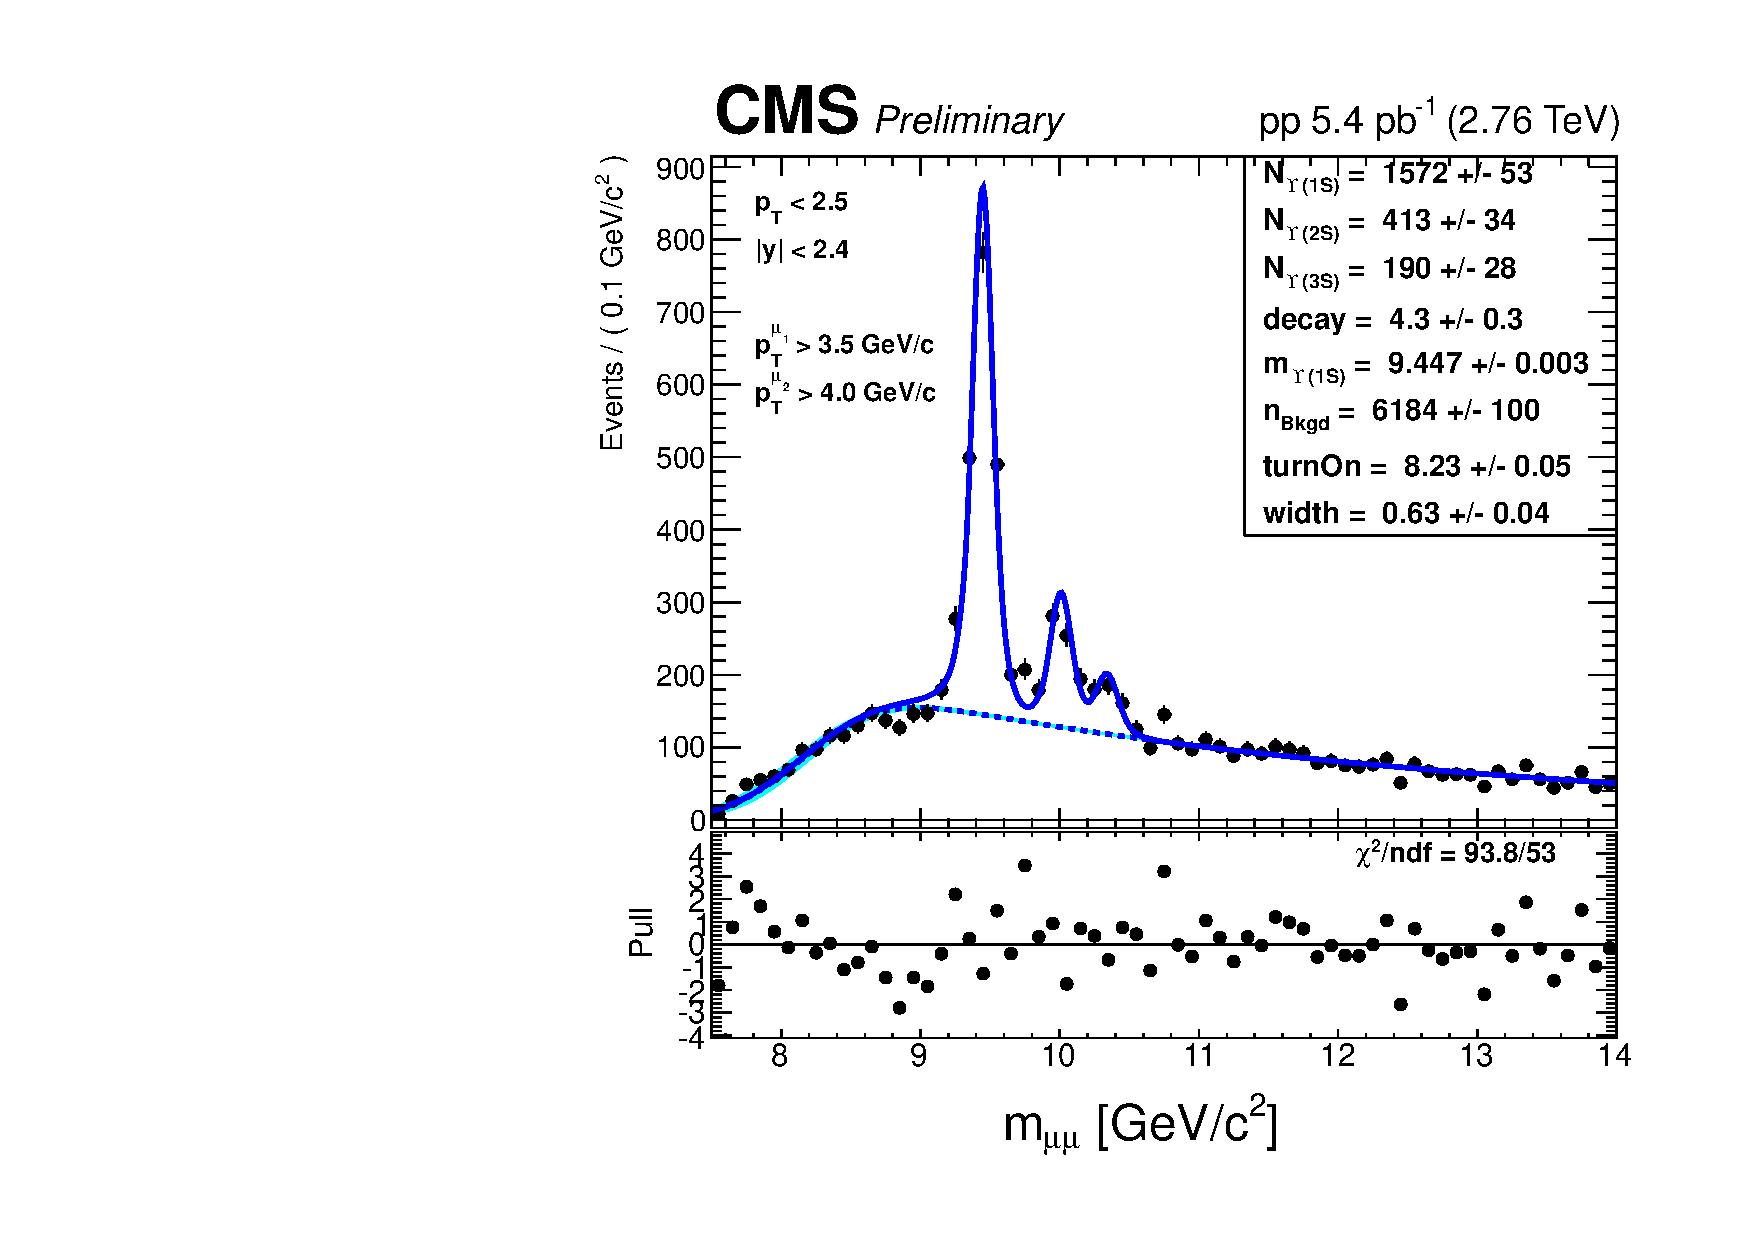
\includegraphics[width=0.49\textwidth]{Chapters/aYield/pp/pt_3p5_4/Pt/Pt_0_2p5/pp2p76tev_Pt_0_2p5_fsr1.pdf}  
  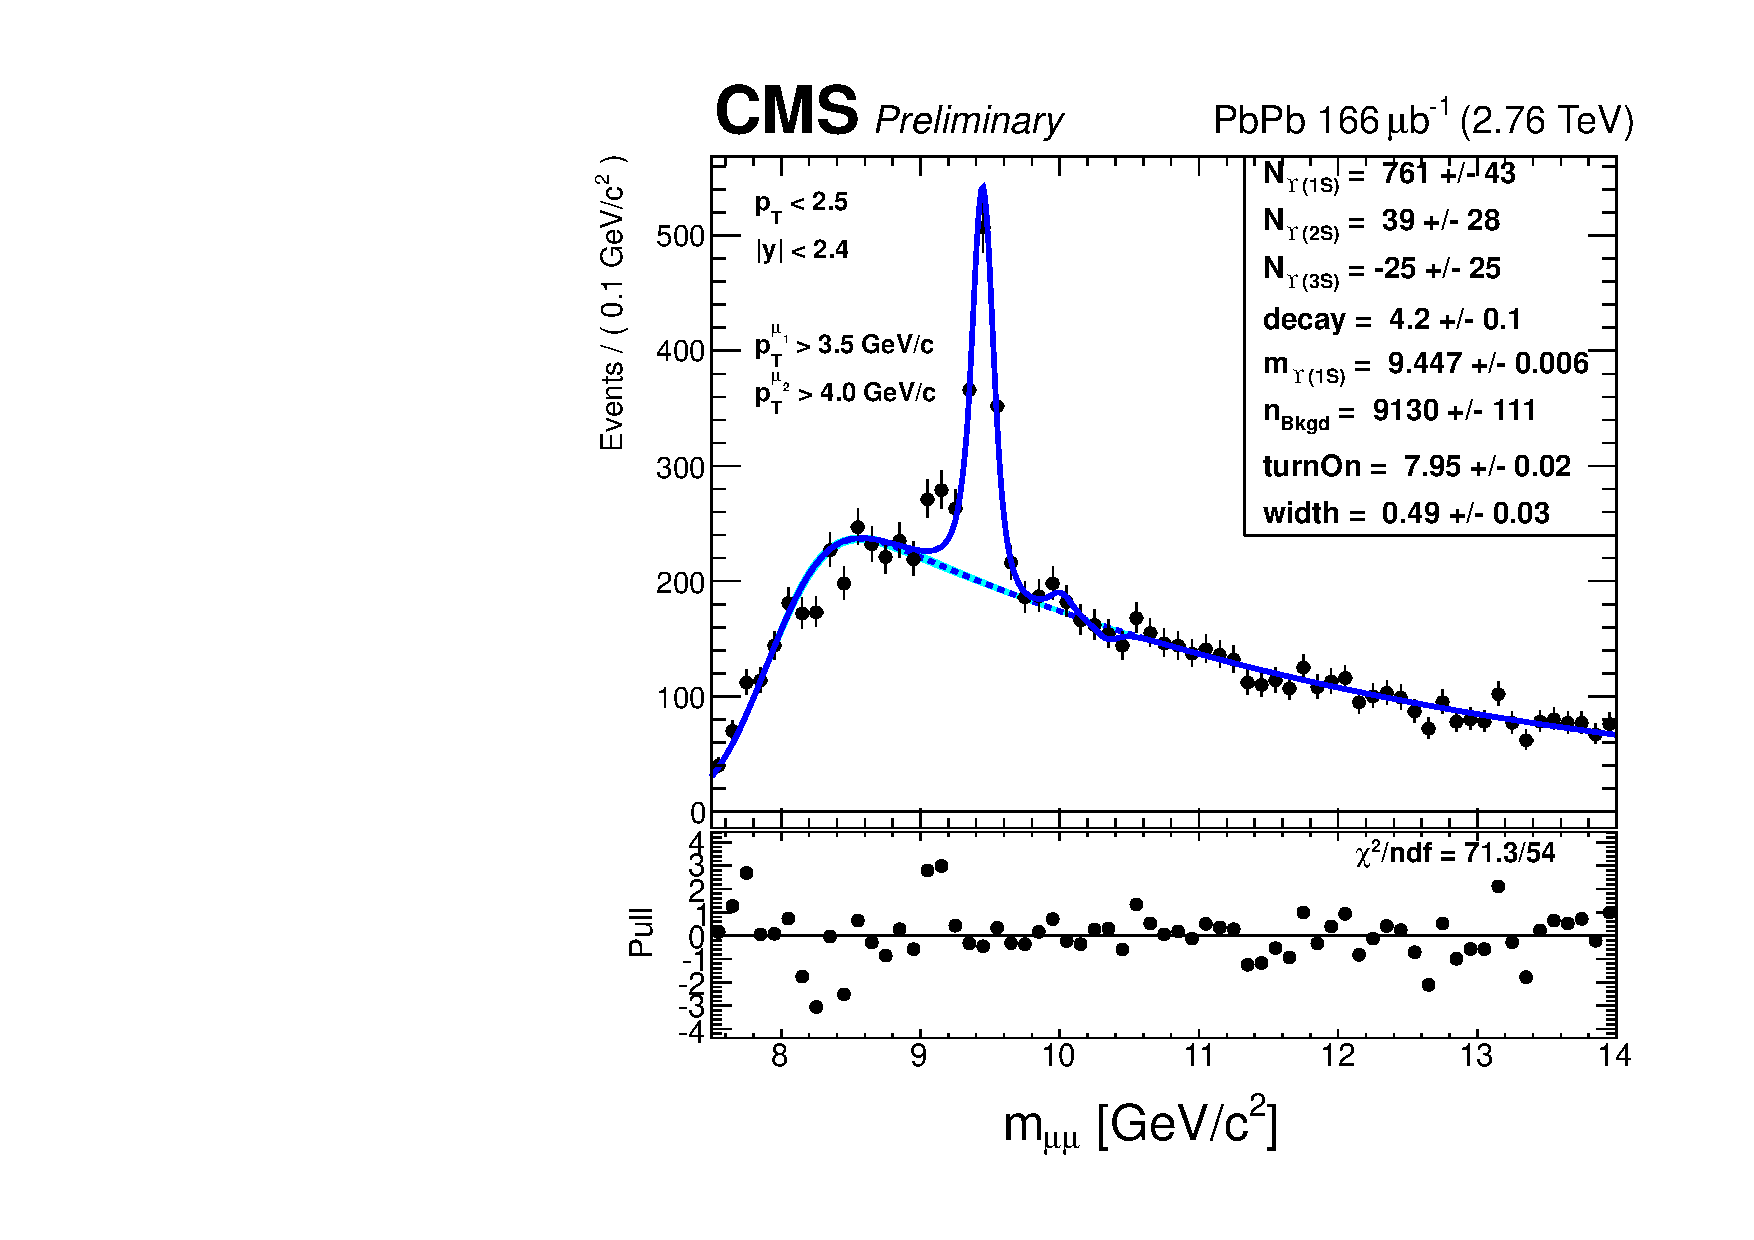
\includegraphics[width=0.49\textwidth]{Chapters/aYield/PbPb/pt_3p5_4/Pt/Pt_0_2p5/PbPb_Pt_0_2p5_fsr1.pdf}
  \caption{Fits to $pp$ (left) and PbPb (right) datasets with loose muon cuts ($\PgUa$ analysis) in the bin $\pt~[{\rm GeV}/c]\in [0 - 2.5]$.}
  \label{fig:YieldsErfExp_pt1Sa} 
\end{figure}
\begin{figure}
  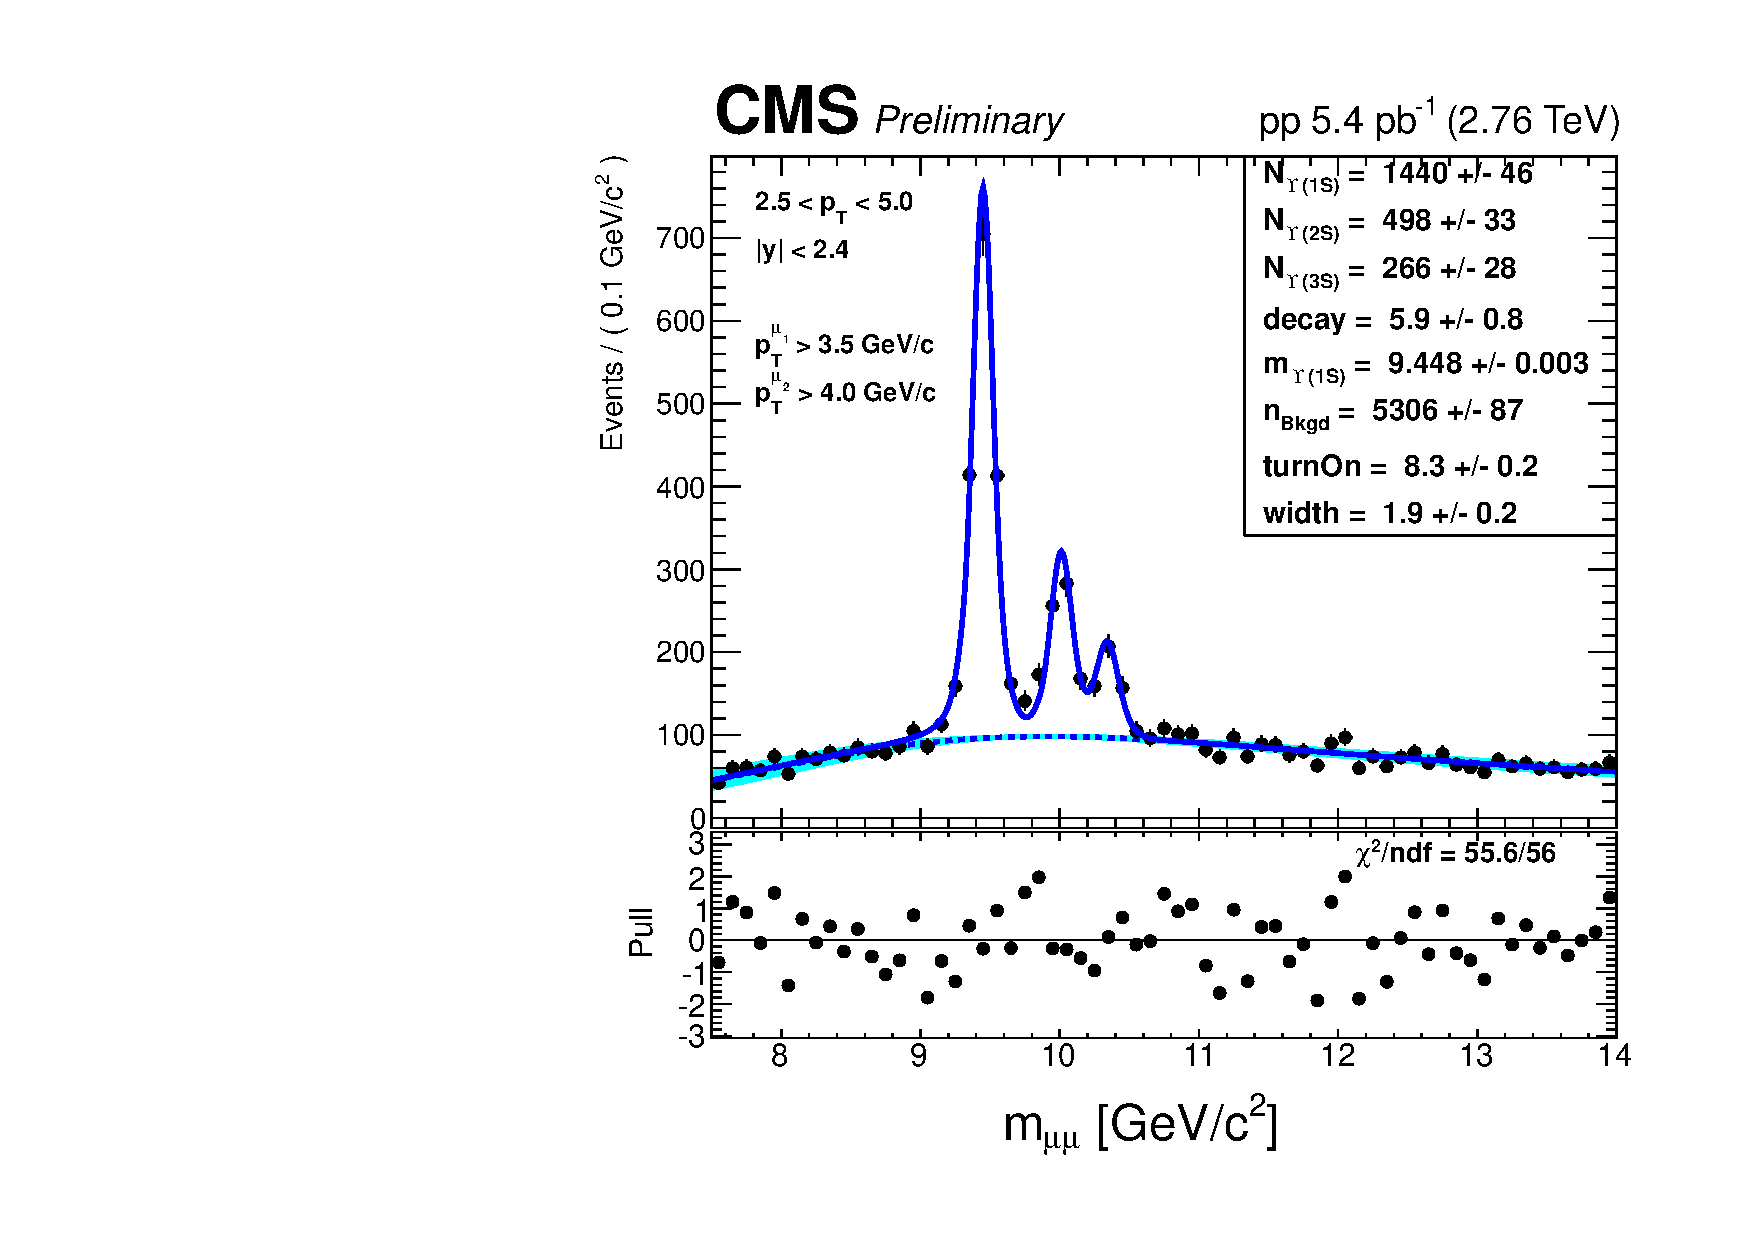
\includegraphics[width=0.49\textwidth]{Chapters/aYield/pp/pt_3p5_4/Pt/Pt_2p5_5/pp2p76tev_Pt_2p5_5_fsr1.pdf}  
  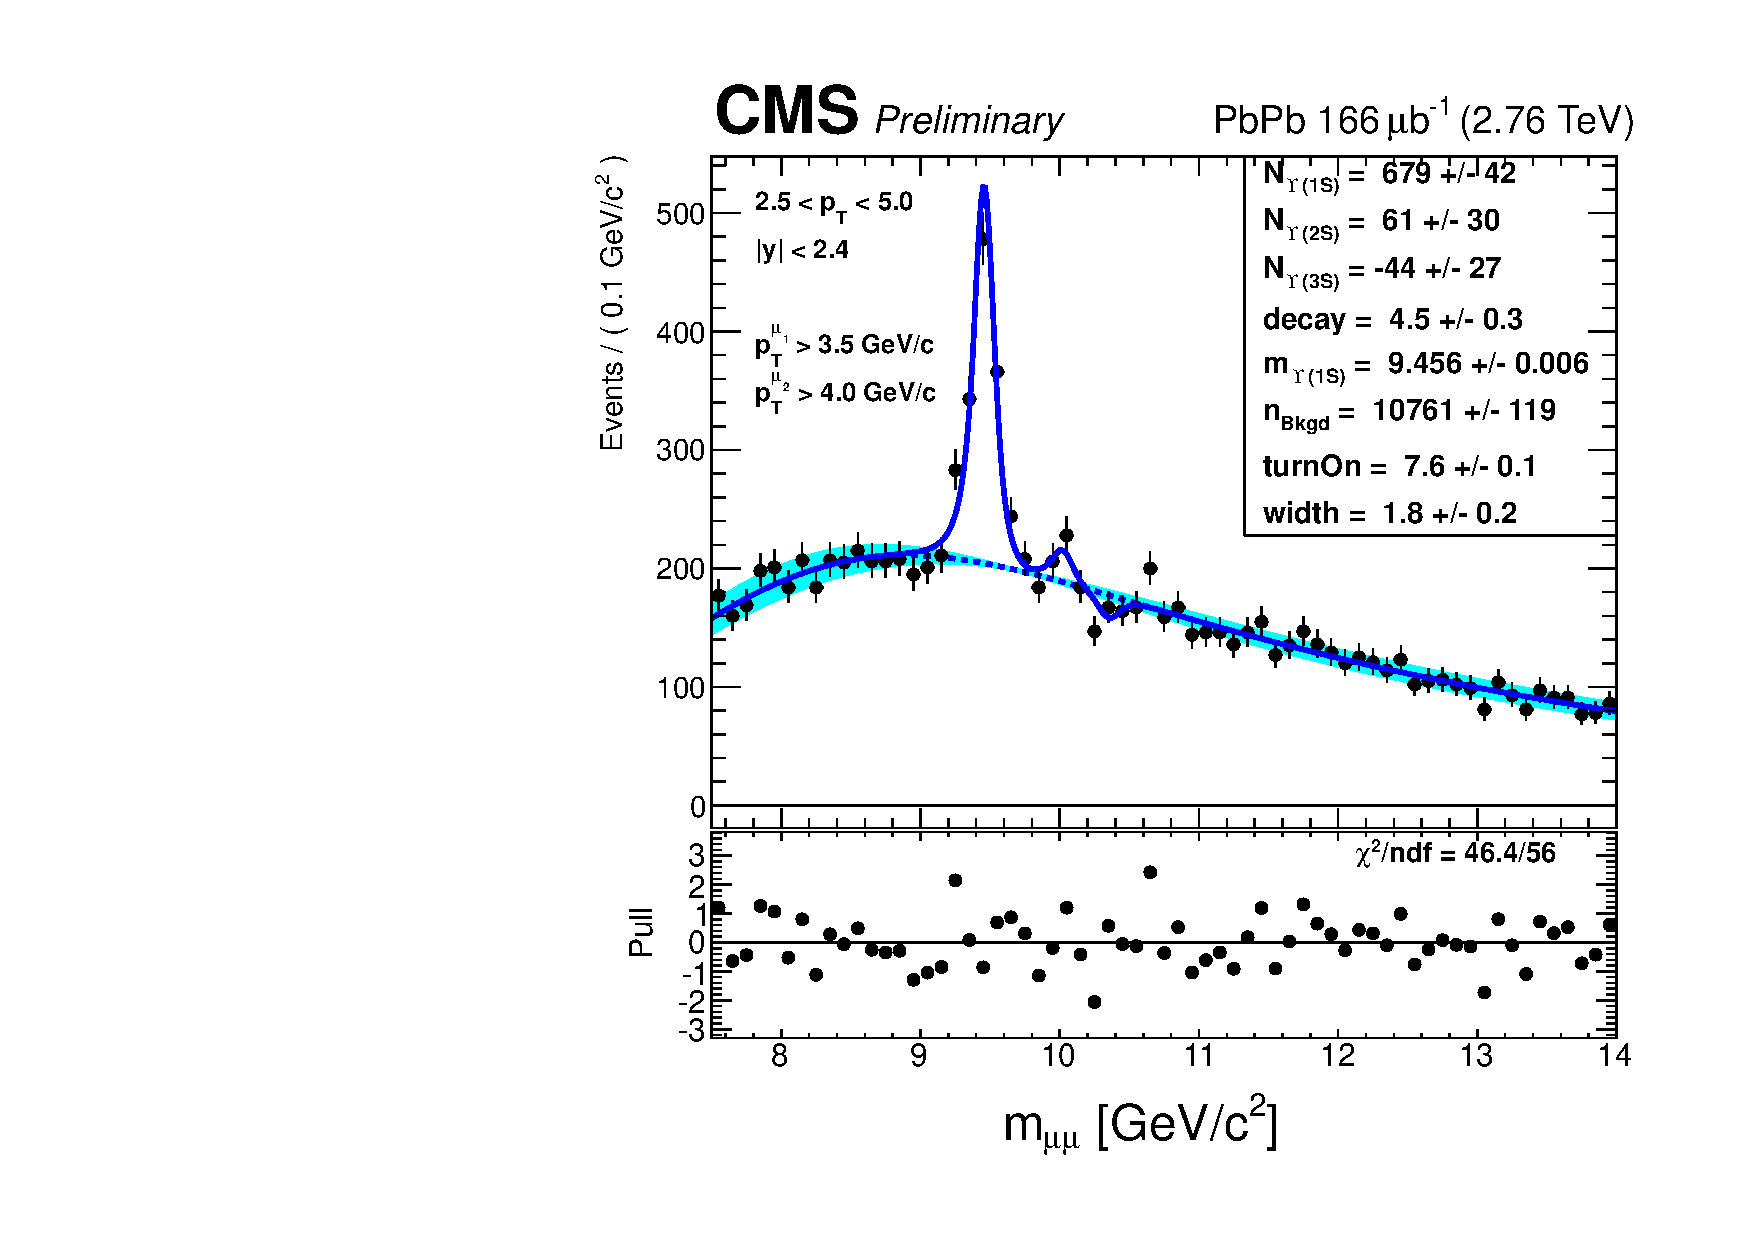
\includegraphics[width=0.49\textwidth]{Chapters/aYield/PbPb/pt_3p5_4/Pt/Pt_2p5_5/PbPb_Pt_2p5_5_fsr1.pdf}
  \caption{Same as Figure~\ref{fig:YieldsErfExp_pt1Sa} in the bin $\pt~[{\rm GeV}/c]\in [2.5 - 5]$.}
  \label{fig:YieldsErfExp_pt1Sb} 
\end{figure}

\begin{figure}
   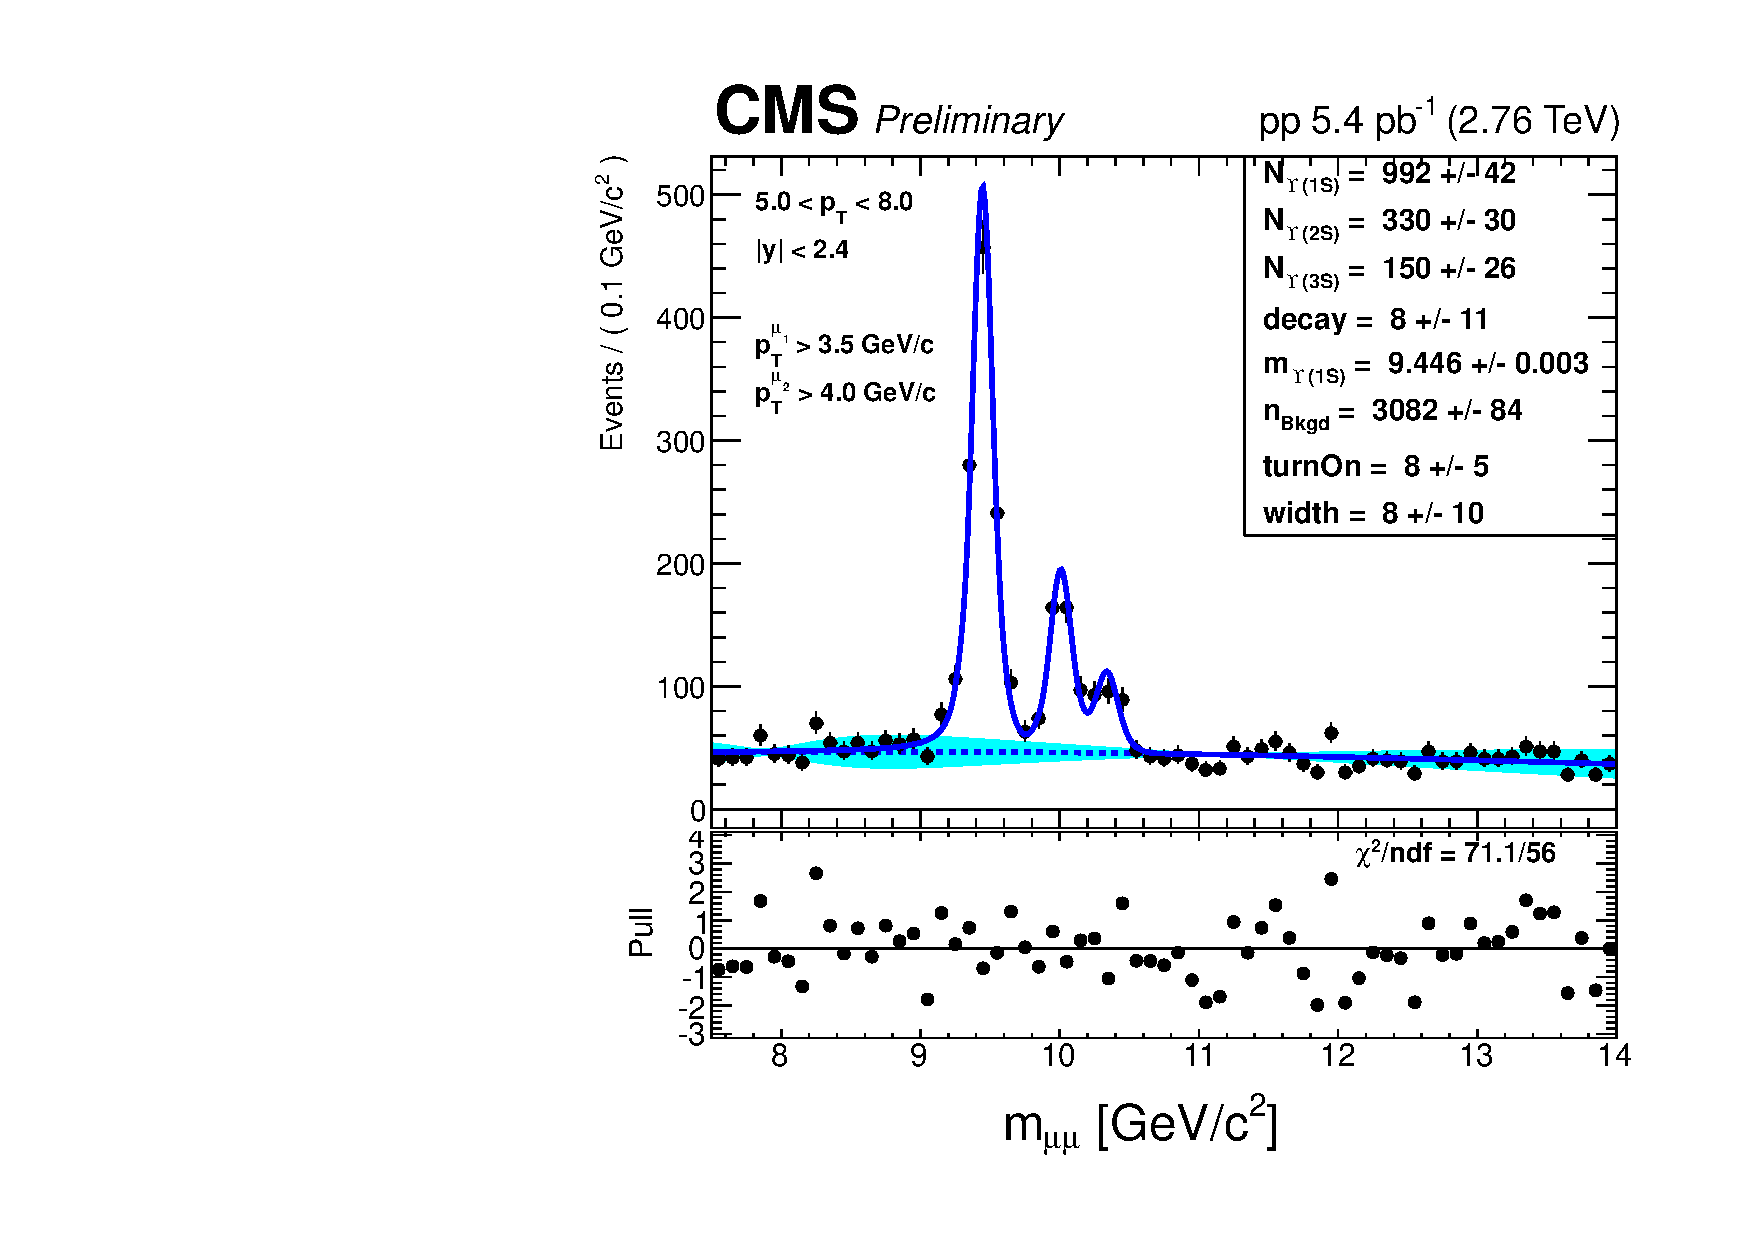
\includegraphics[width=0.49\textwidth]{Chapters/aYield/pp/pt_3p5_4/Pt/Pt_5_8/pp2p76tev_Pt_5_8_fsr1.pdf}  
  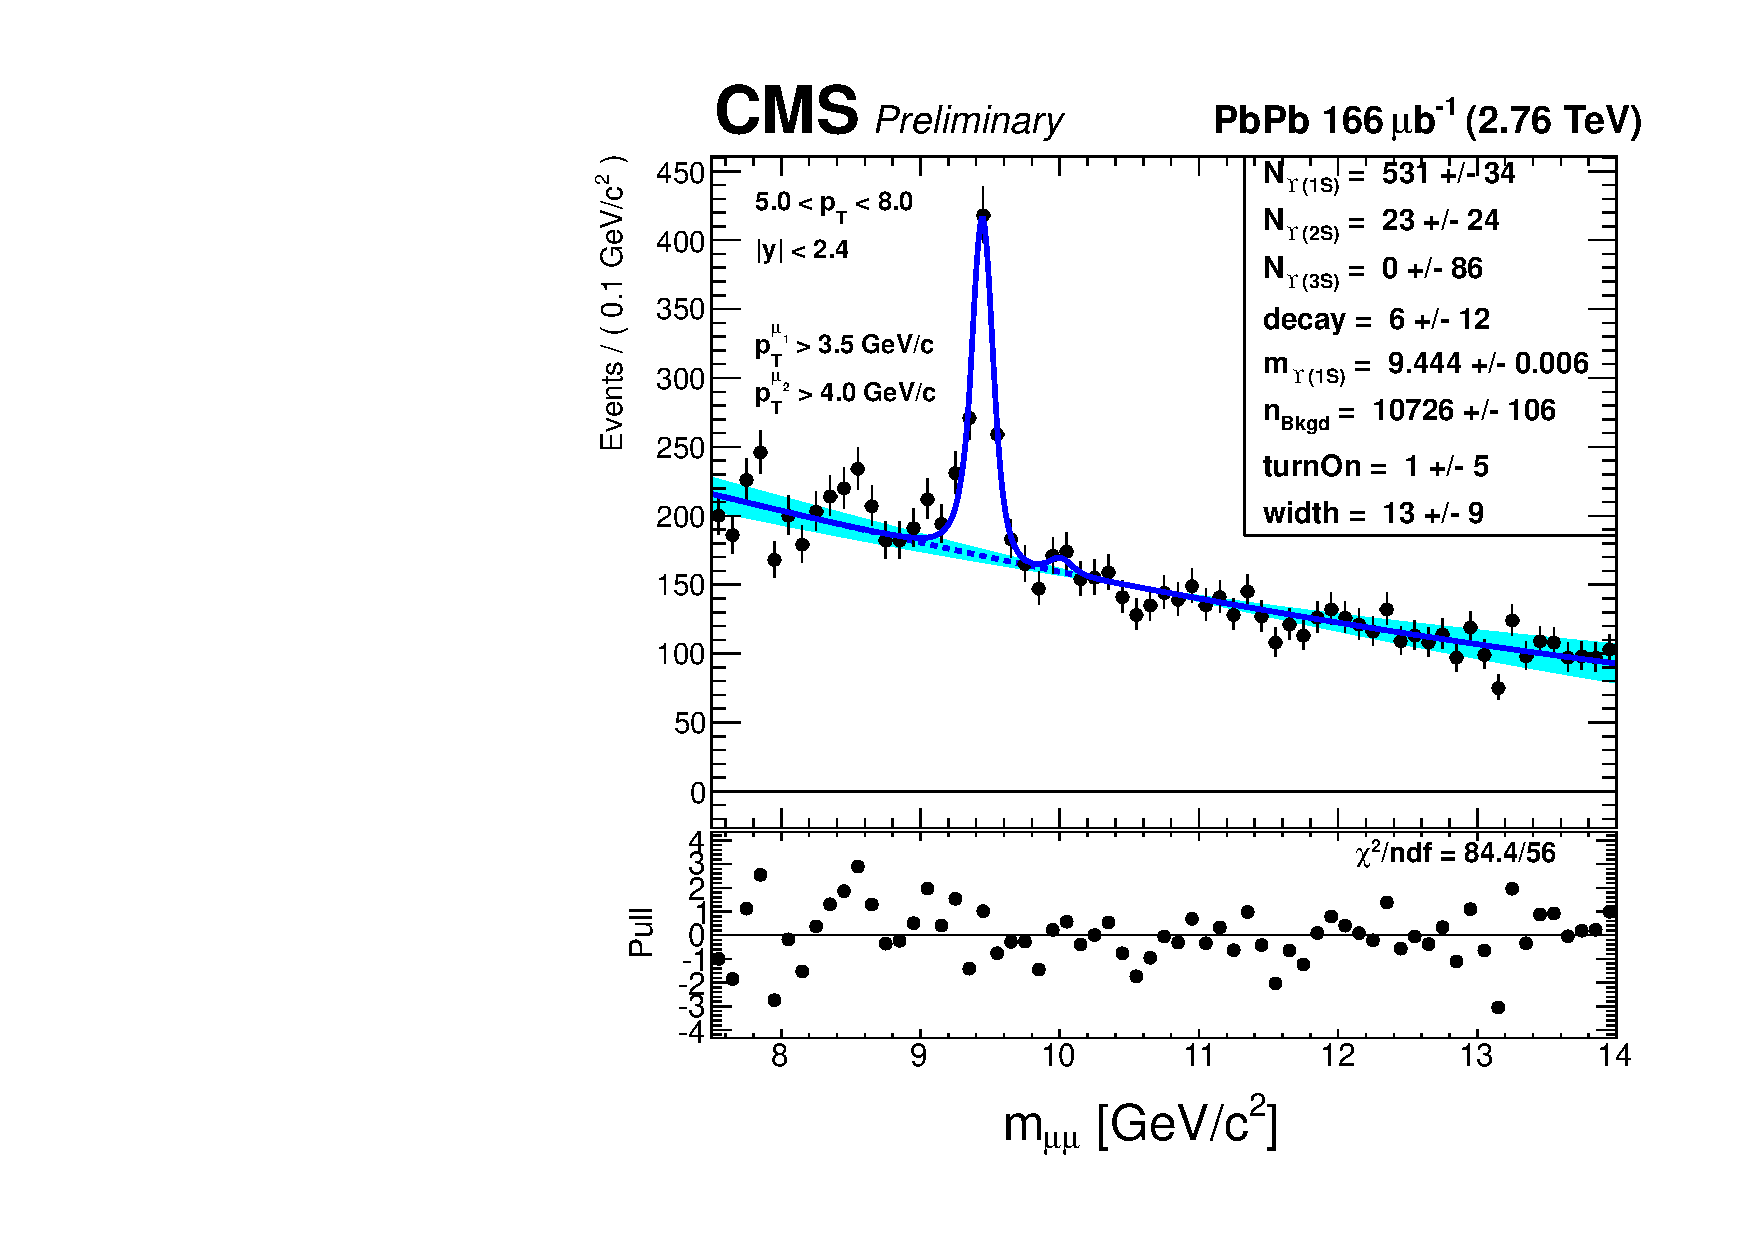
\includegraphics[width=0.49\textwidth]{Chapters/aYield/PbPb/pt_3p5_4/Pt/Pt_5_8/PbPb_Pt_5_8_fsr1.pdf}
 
  \caption{Same as Figure~\ref{fig:YieldsErfExp_pt1Sa} in the bin $\pt~[{\rm GeV}/c]\in [5 - 8]$.}
  \label{fig:YieldsErfExp_pt1Sc} 
\end{figure}
\begin{figure}
  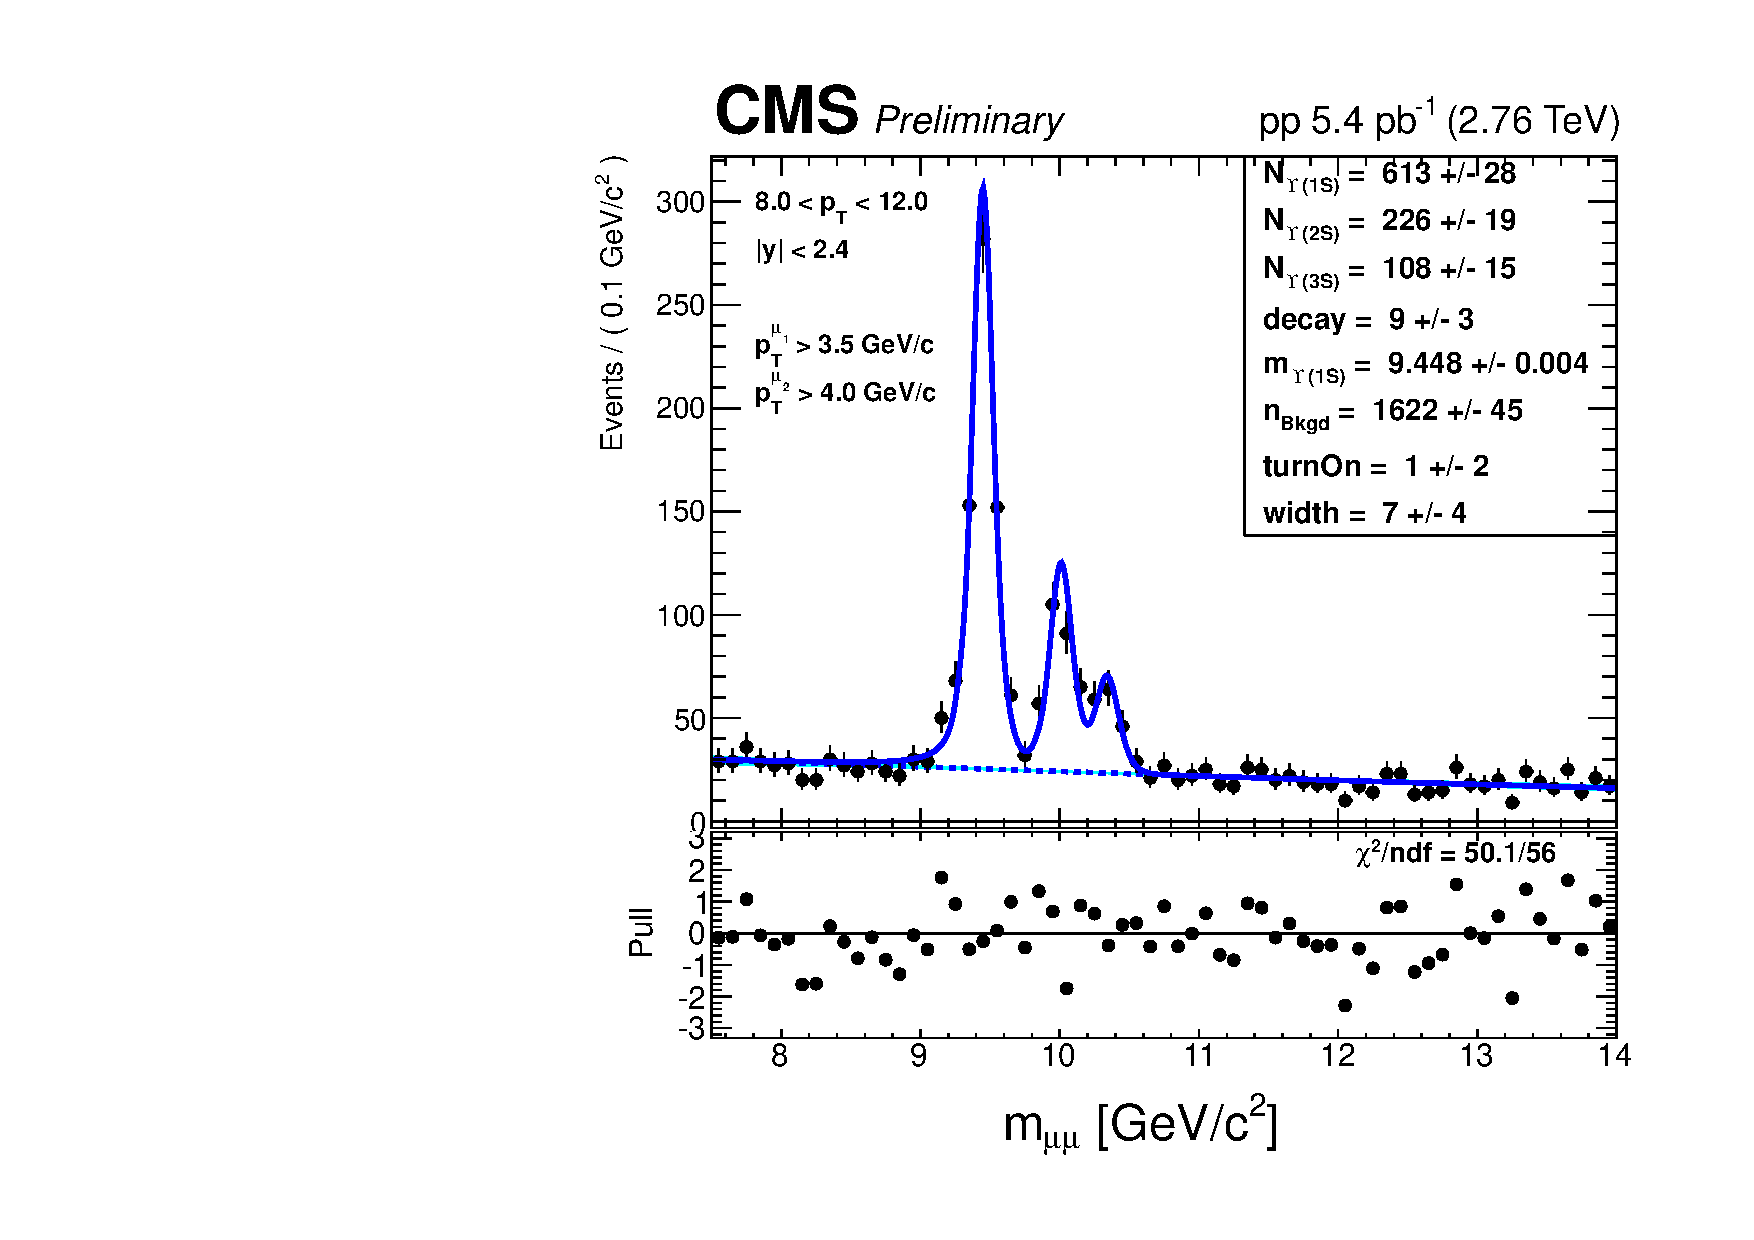
\includegraphics[width=0.49\textwidth]{Chapters/aYield/pp/pt_3p5_4/Pt/Pt_8_12/pp2p76tev_Pt_8_12_fsr1.pdf}  
  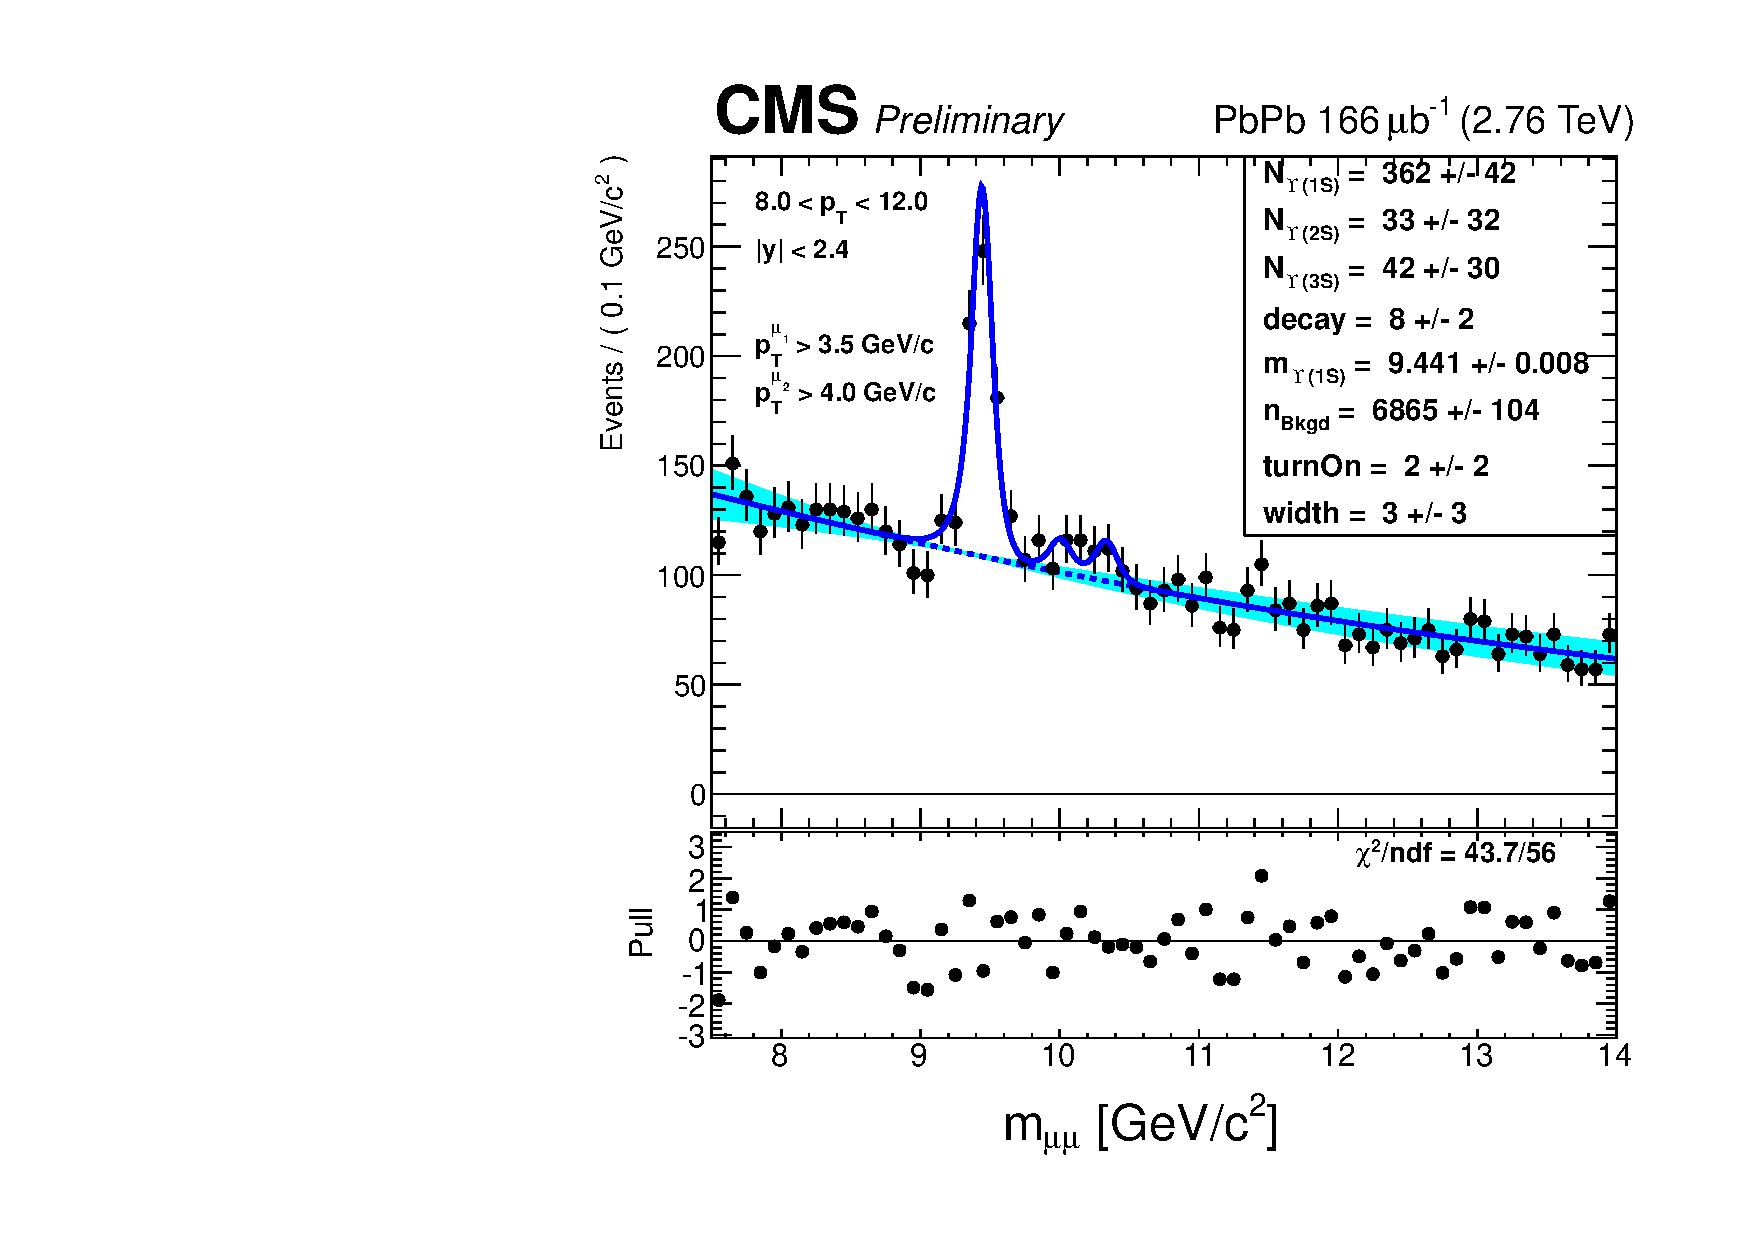
\includegraphics[width=0.49\textwidth]{Chapters/aYield/PbPb/pt_3p5_4/Pt/Pt_8_12/PbPb_Pt_8_12_fsr1.pdf}
  \caption{Same as Figure~\ref{fig:YieldsErfExp_pt1Sa} in the bin $\pt~[{\rm GeV}/c]\in [8 - 12]$.}
  \label{fig:YieldsErfExp_pt1Sd} 
\end{figure}
\begin{figure}
  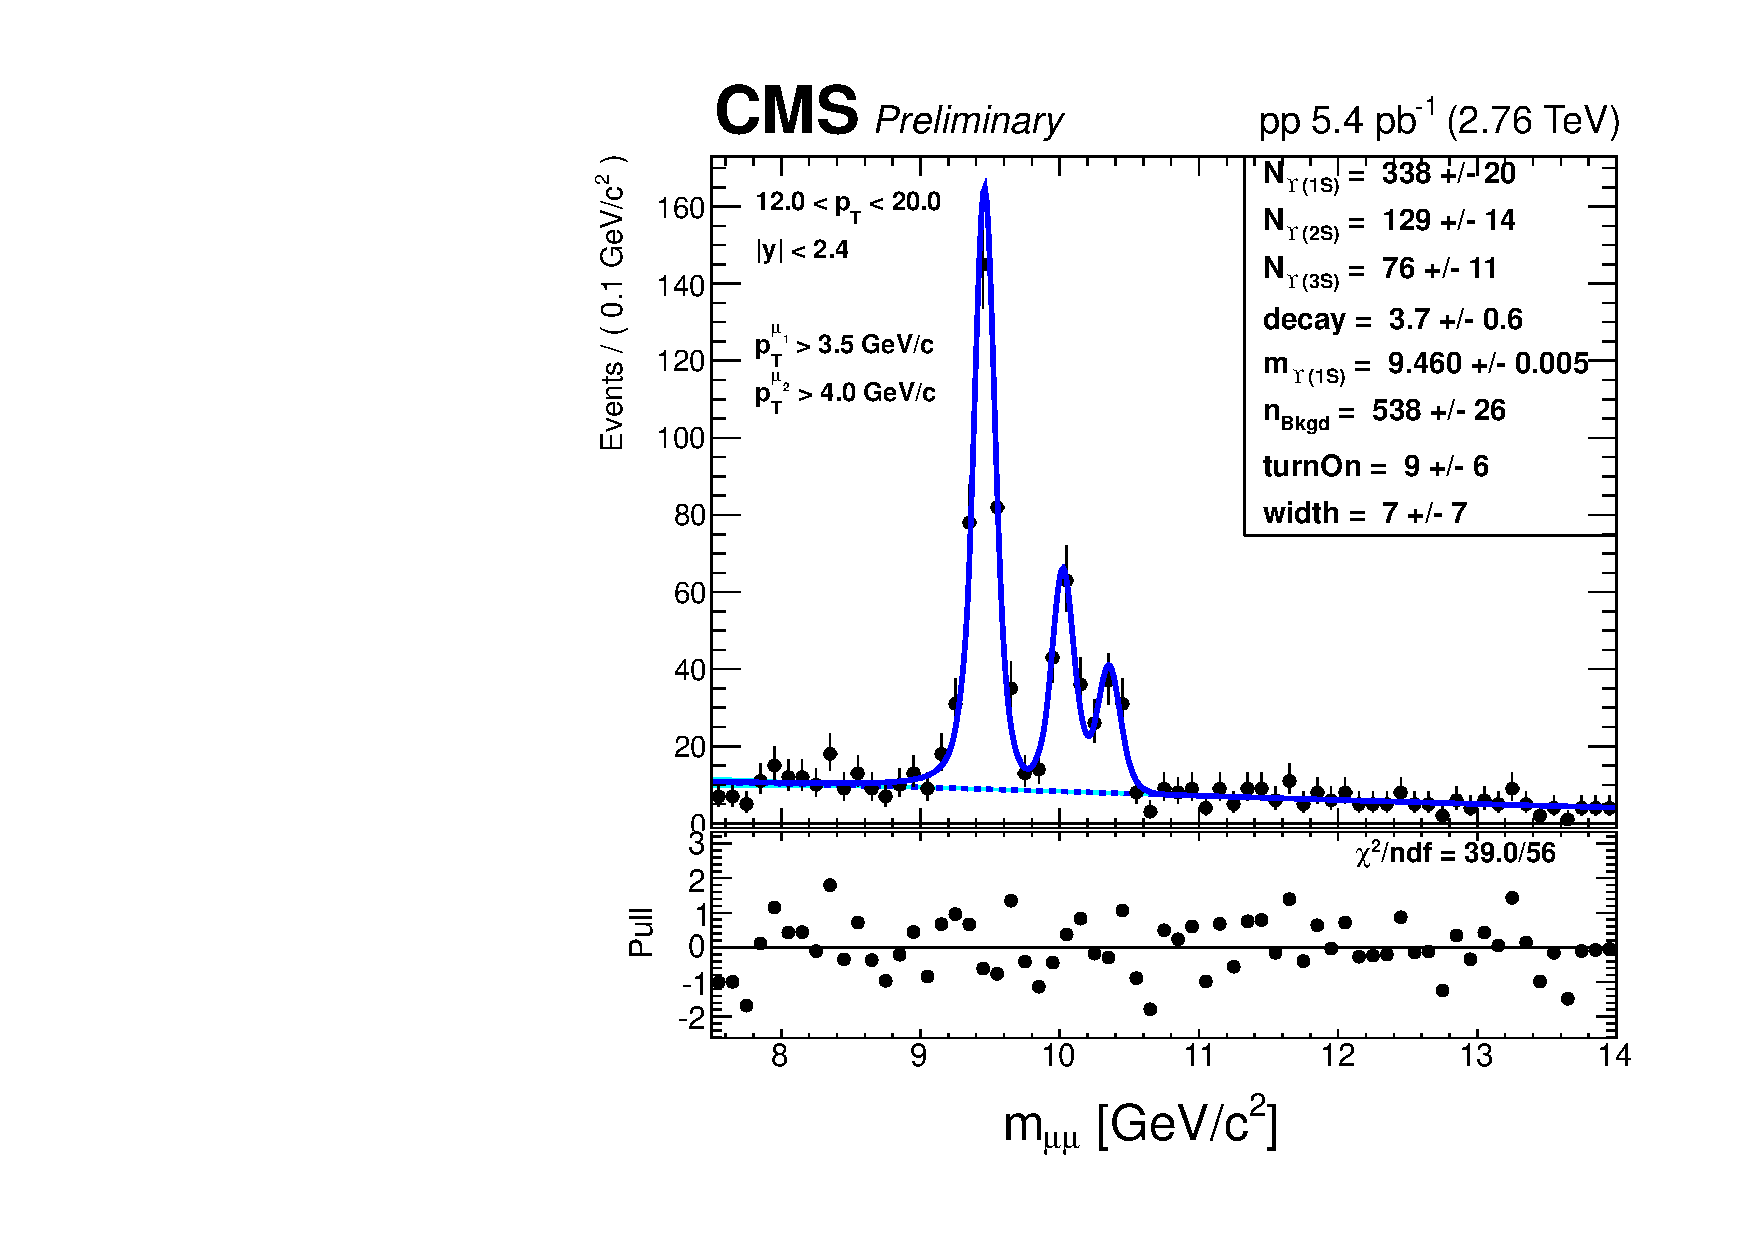
\includegraphics[width=0.49\textwidth]{Chapters/aYield/pp/pt_3p5_4/Pt/Pt_12_20/pp2p76tev_Pt_12_20_fsr1.pdf}  
  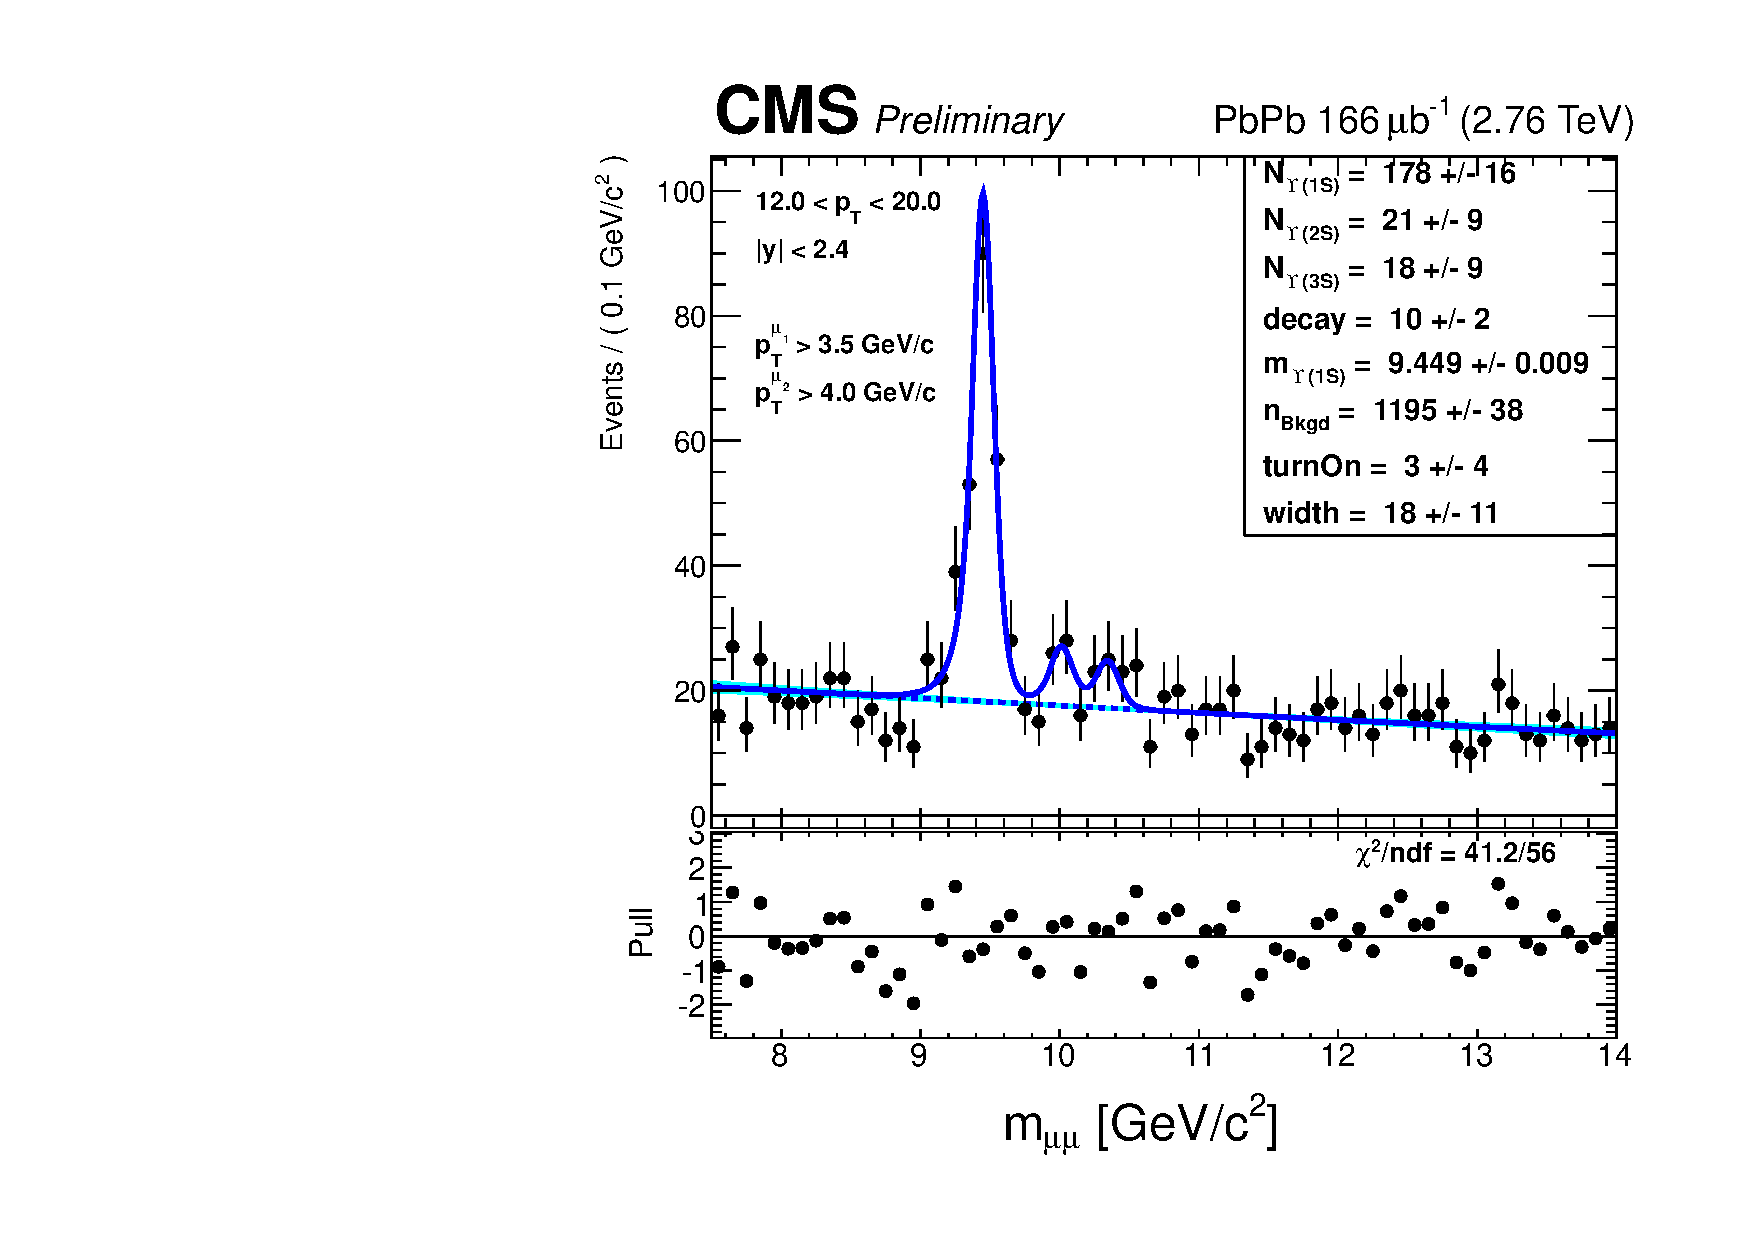
\includegraphics[width=0.49\textwidth]{Chapters/aYield/PbPb/pt_3p5_4/Pt/Pt_12_20/PbPb_Pt_12_20_fsr1.pdf}
  \caption{Same as Figure~\ref{fig:YieldsErfExp_pt1Sa} in the bin $\pt~[{\rm GeV}/c]\in [12 - 20]$.}
  \label{fig:YieldsErfExp_pt1Se} 
\end{figure}
\clearpage

Figures from~\ref{fig:YieldsErfExp_pt2Sa} to~\ref{fig:YieldsErfExp_pt2Sc}
present the three \pt\ bins of the \PgUb\ analysis in PbPb collisions.
\begin{figure}
  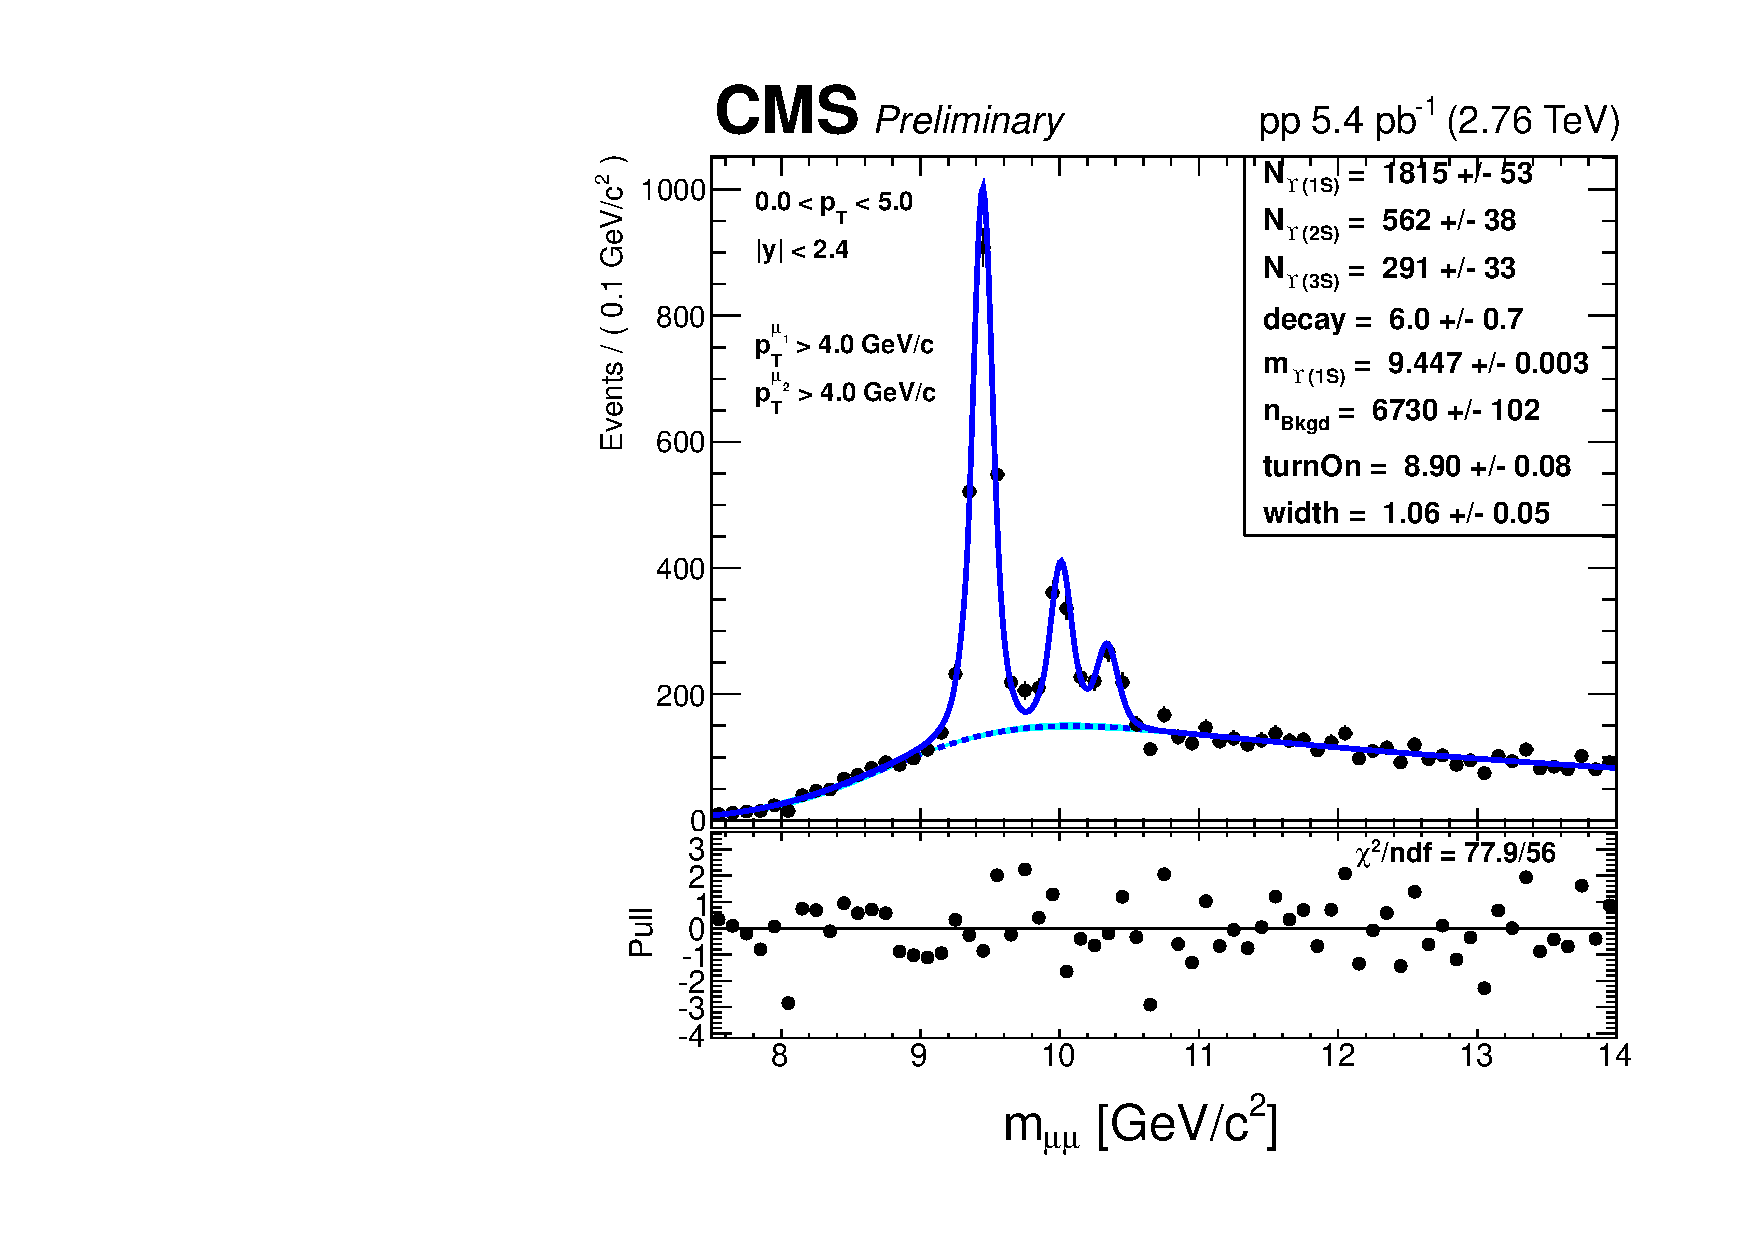
\includegraphics[width=0.49\textwidth]{Chapters/aYield/pp/pt_4_4/Pt/Pt_0_5/pp2p76tev_Pt_0_5_fsr1.pdf}  
  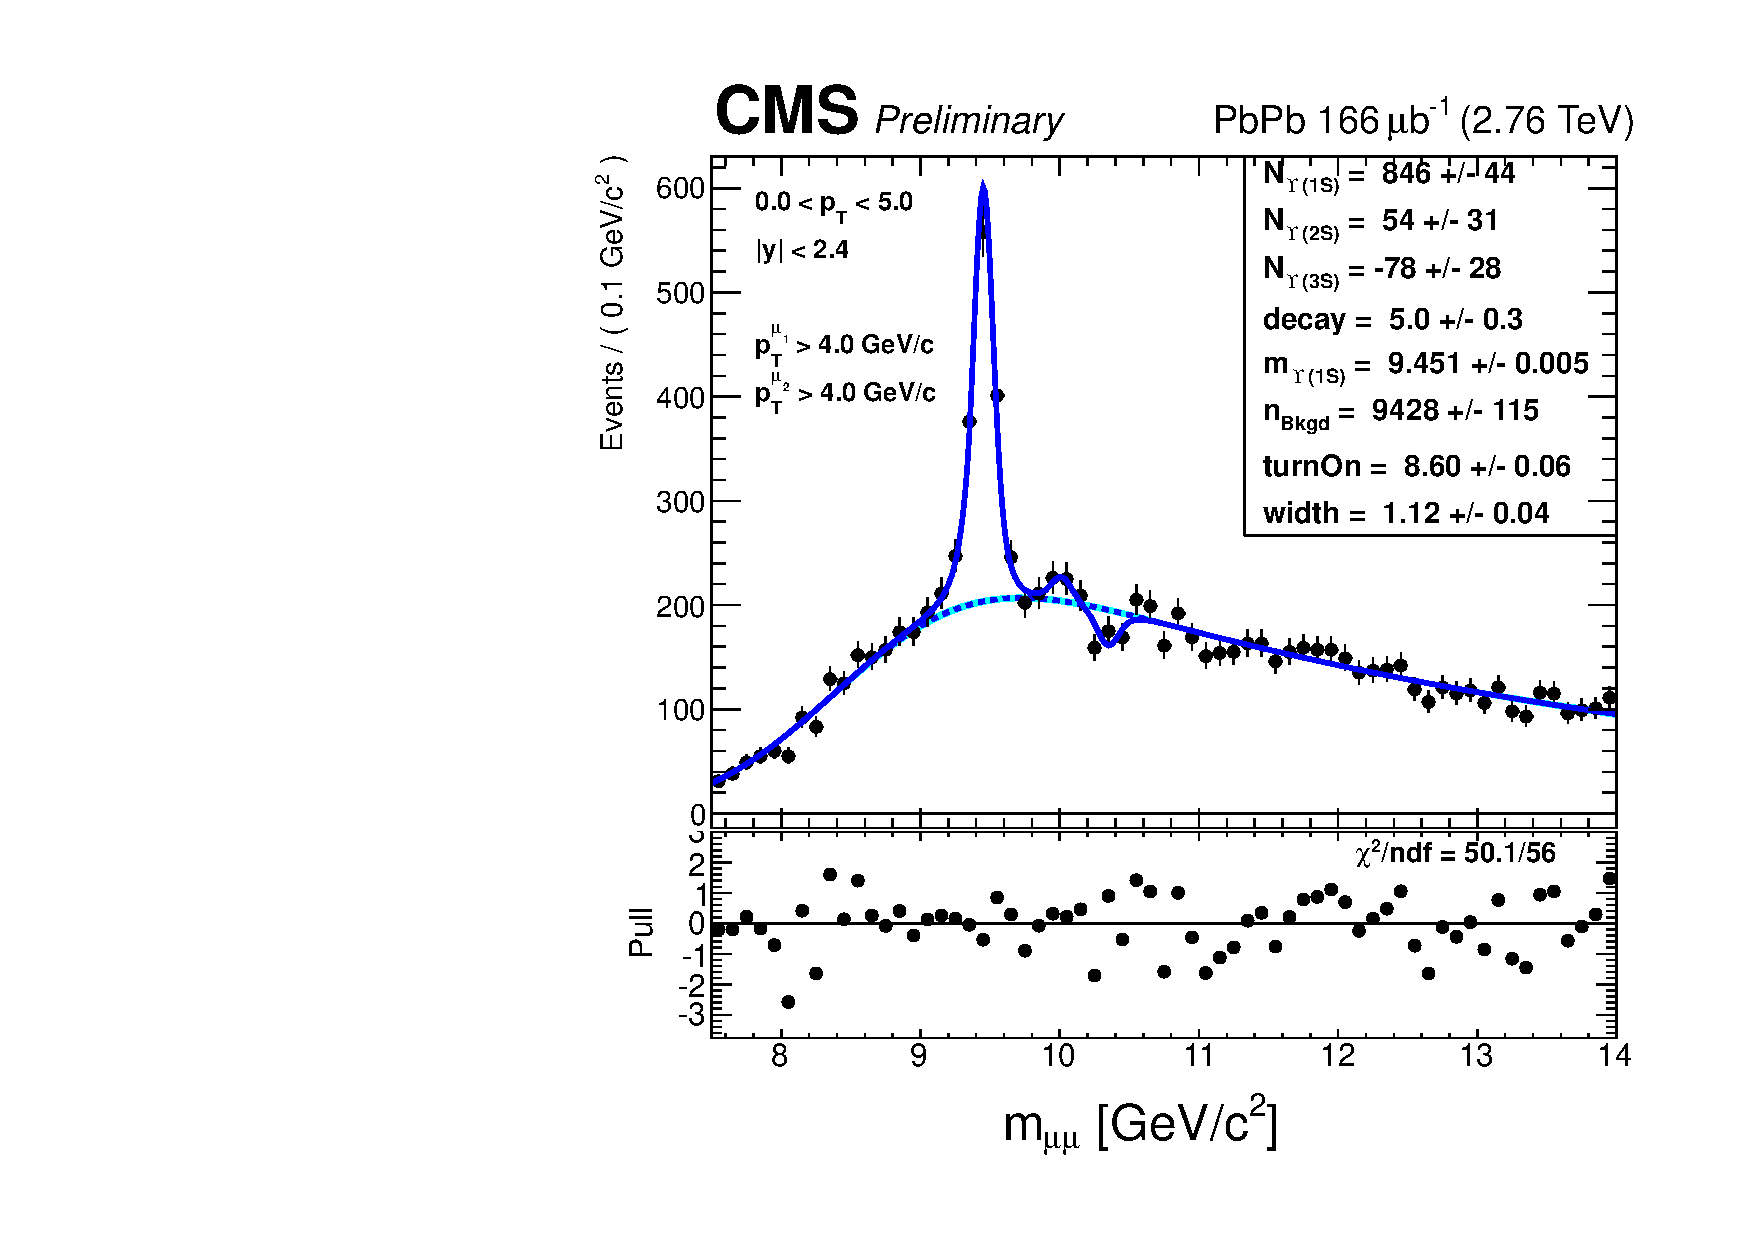
\includegraphics[width=0.49\textwidth]{Chapters/aYield/PbPb/pt_4_4/Pt/Pt_0_5/PbPb_Pt_0_5_fsr1.pdf}
  \caption{Fits to pp (left) and PbPb (right) datasets with tight muon cuts ($\PgUb$ analysis) in the bin $\pt~[{\rm GeV}/c]\in [0 - 5]$.}
  \label{fig:YieldsErfExp_pt2Sa} 
\end{figure}
\begin{figure}
  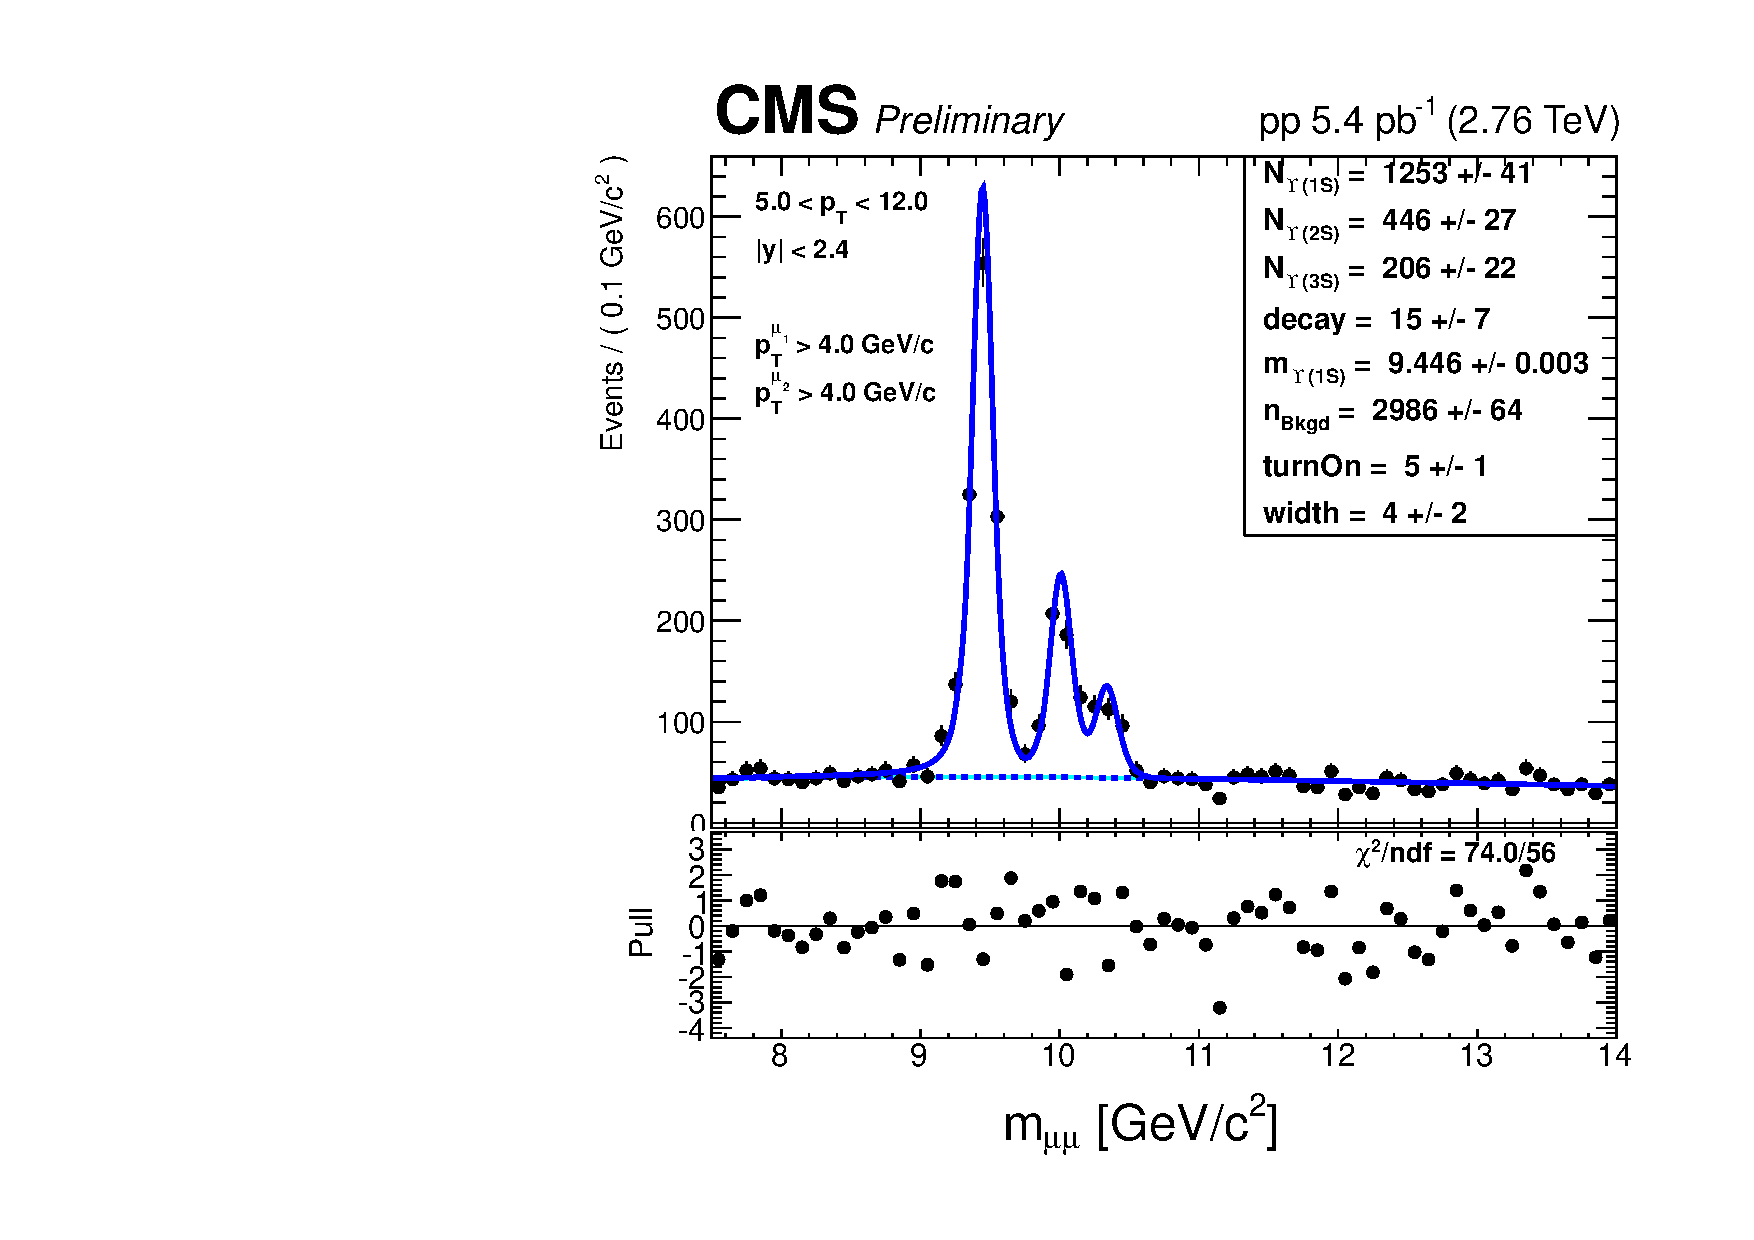
\includegraphics[width=0.49\textwidth]{Chapters/aYield/pp/pt_4_4/Pt/Pt_5_12/pp2p76tev_Pt_5_12_fsr1.pdf}  
  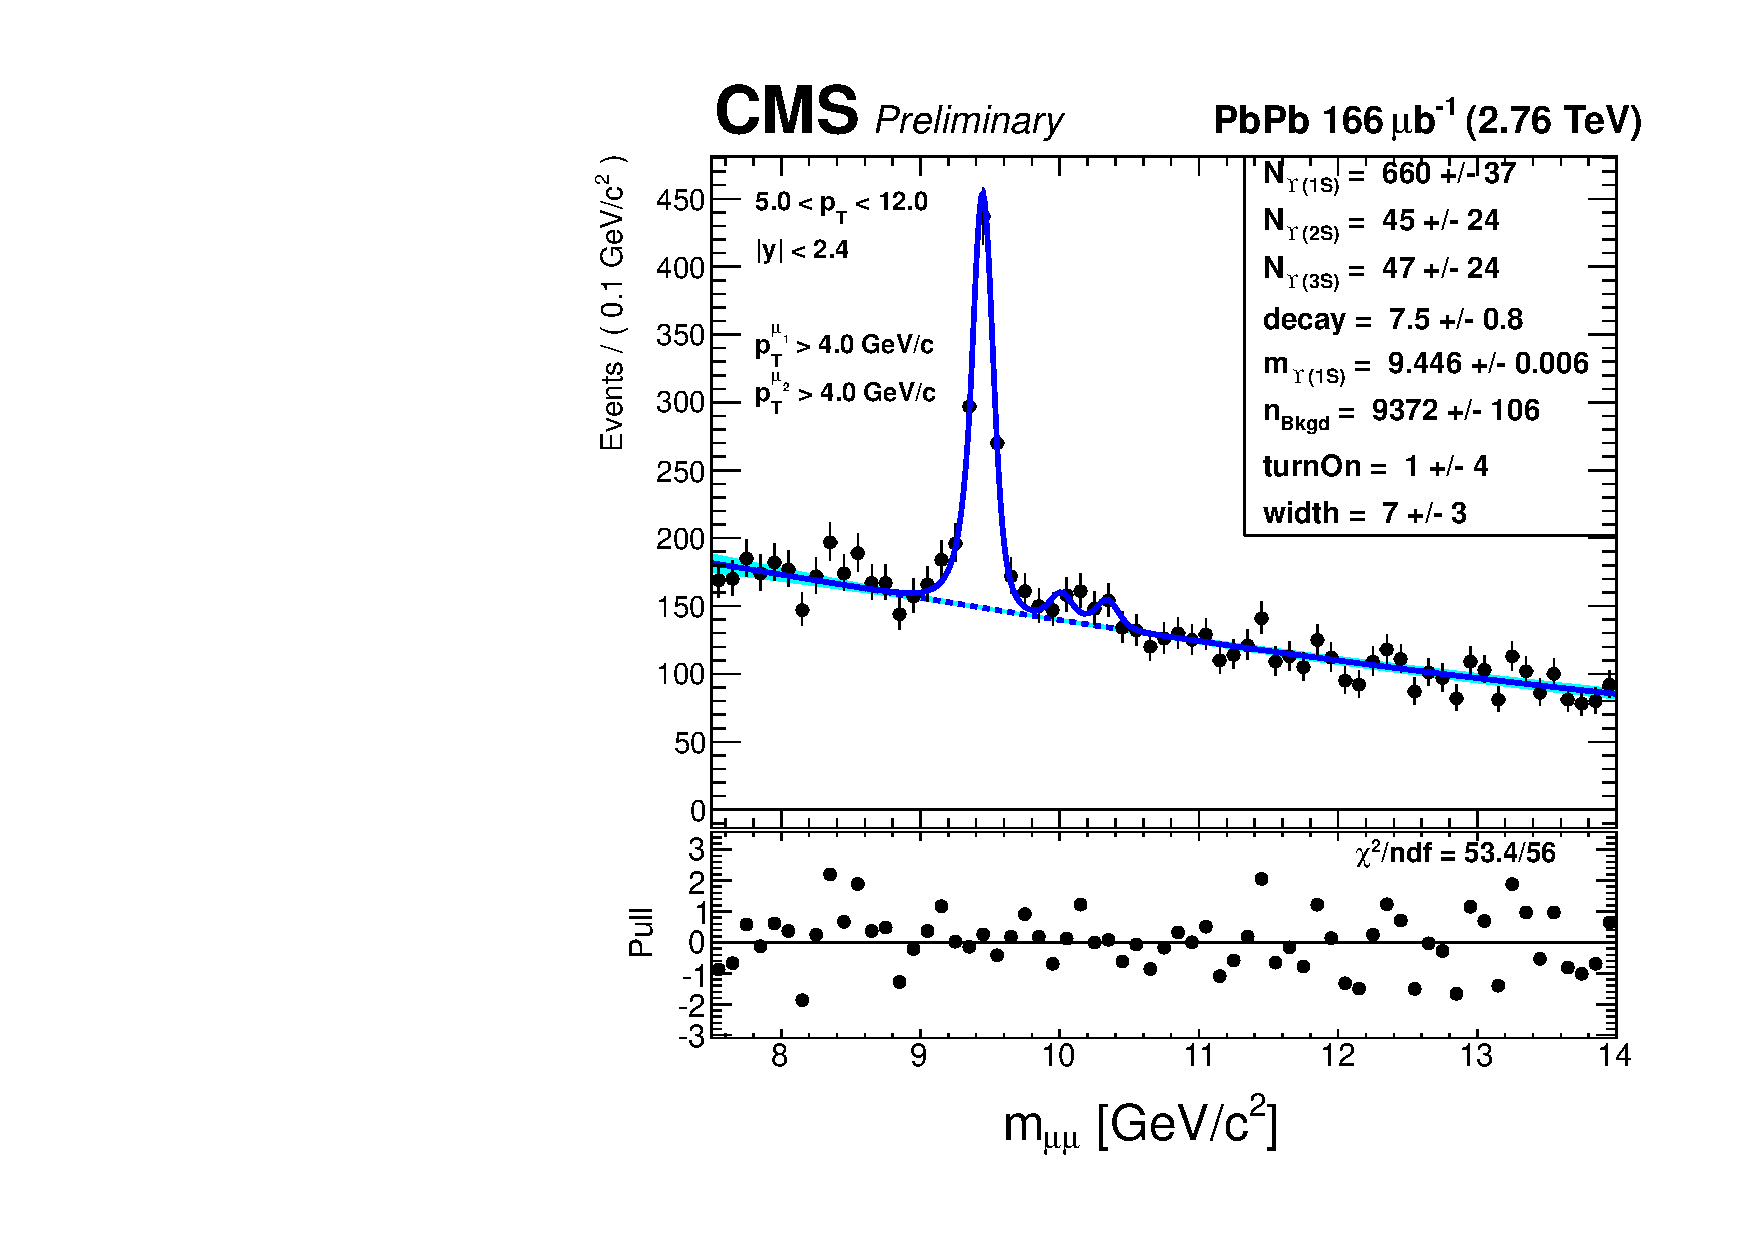
\includegraphics[width=0.49\textwidth]{Chapters/aYield/PbPb/pt_4_4/Pt/Pt_5_12/PbPb_Pt_5_12_fsr1.pdf} 
  \caption{Same as Figure~\ref{fig:YieldsErfExp_pt2Sa} in the bin $\pt~[{\rm GeV}/c]\in [5 - 12]$.}
  \label{fig:YieldsErfExp_pt2Sb} 
\end{figure}
\begin{figure}
  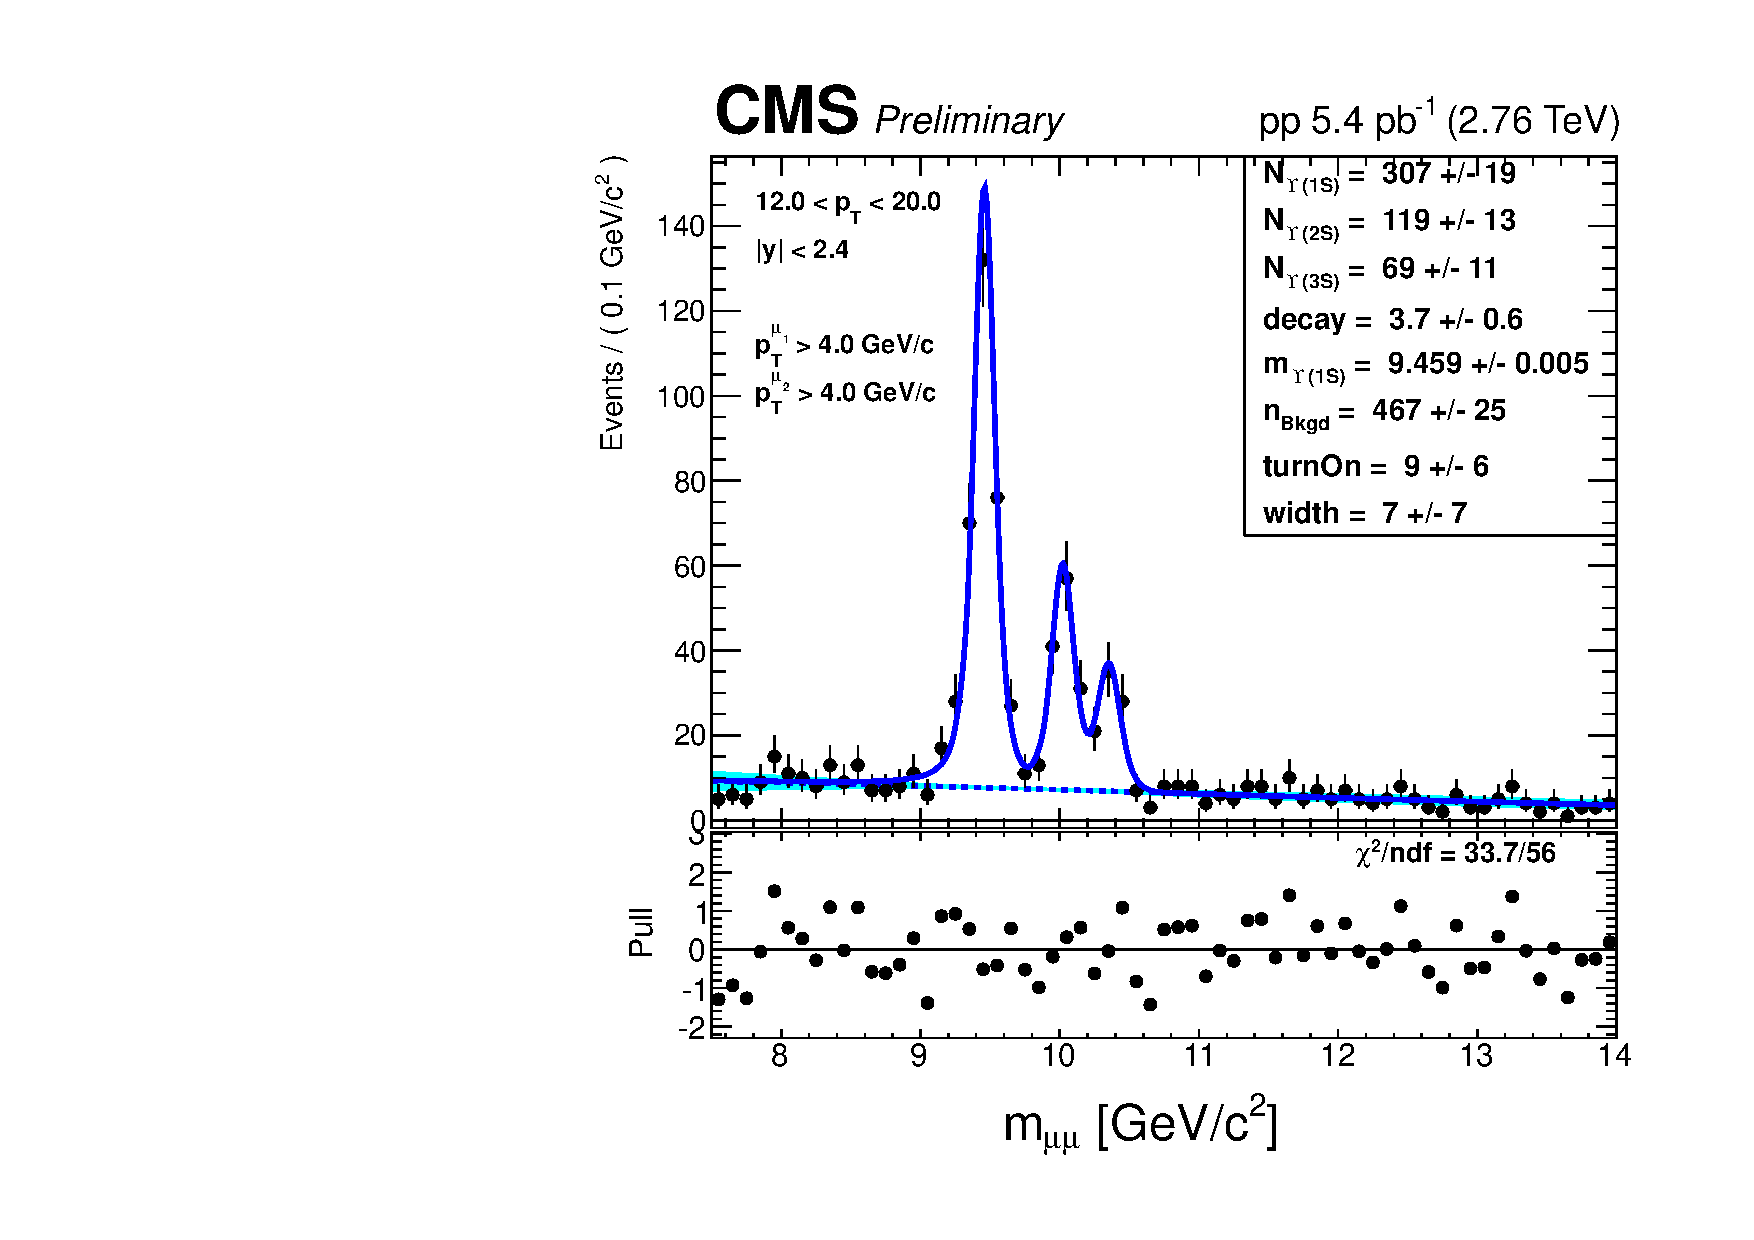
\includegraphics[width=0.49\textwidth]{Chapters/aYield/pp/pt_4_4/Pt/Pt_12_20/pp2p76tev_Pt_12_20_fsr1.pdf}  
  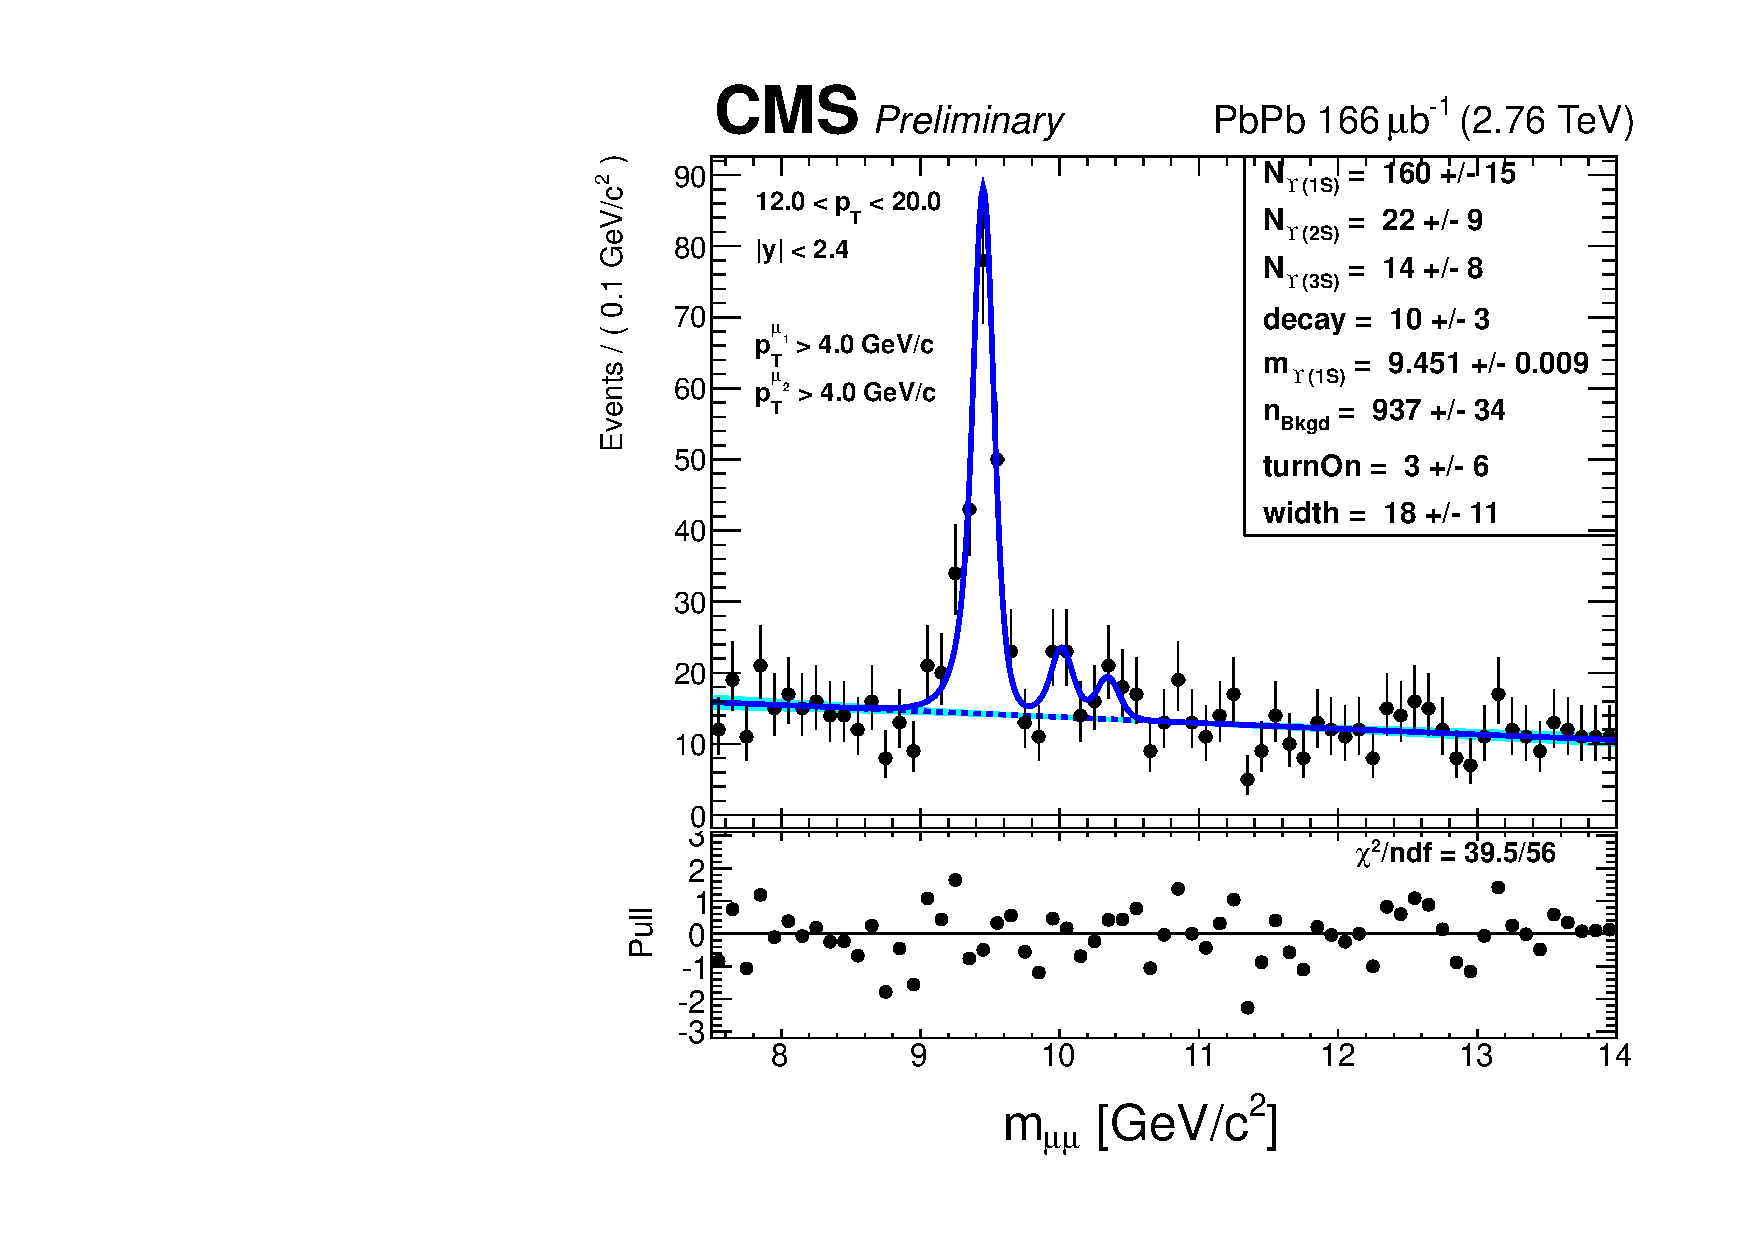
\includegraphics[width=0.49\textwidth]{Chapters/aYield/PbPb/pt_4_4/Pt/Pt_12_20/PbPb_Pt_12_20_fsr1.pdf} 
  \caption{Same as Figure~\ref{fig:YieldsErfExp_pt2Sa} in the bin $\pt~[{\rm GeV}/c]\in [12 - 20]$.}
  \label{fig:YieldsErfExp_pt2Sc} 
\end{figure}

Figure~\ref{fig:extrabin}: Bin $20 < \pt < 50$ \GeVc, not included in
analysis so far.
\begin{figure}
\begin{centering}  
  \includegraphics[width=0.49\textwidth]{Chapters/aUpsilon/yield_m8_14_pp2p76tev_cent0M40_bkgModel3_sigModel4_muonEtaM240240_muonPt350M400_dimuPt20005000_dimuY000240_trkRot0_constrain0_fsr1_sigma0_ref2_pulls.pdf}
  \includegraphics[width=0.49\textwidth]{Chapters/aUpsilon/yield_m8_14_pbpbRegit_cm_cent0M100_bkgModel3_sigModel4_muonEtaM240240_muonPt350M400_dimuPt20005000_dimuY000240_trkRot0_constrain0_fsr1_sigma0_ref2_pulls.pdf}
  \caption{\PgU\ raw yields in the $20 < \pt < 50 \GeVc$ bin. Left:
    pp, right: PbPb. These events are not included in the present analysis.}
  \label{fig:extrabin}
\end{centering}  
\end{figure}

\subsection{Rapidity dependent analysis of $pp$ and PbPb
  yields}
\label{sec:figs_y}
The following Figures~\ref{fig:YieldsErfExp_y1Sa} to ~\ref{fig:YieldsErfExp_y1Sf} are used in the computation of the rapidity
dependent cross section for \PgUa\ and its corresponding \RAA.
\begin{figure}
  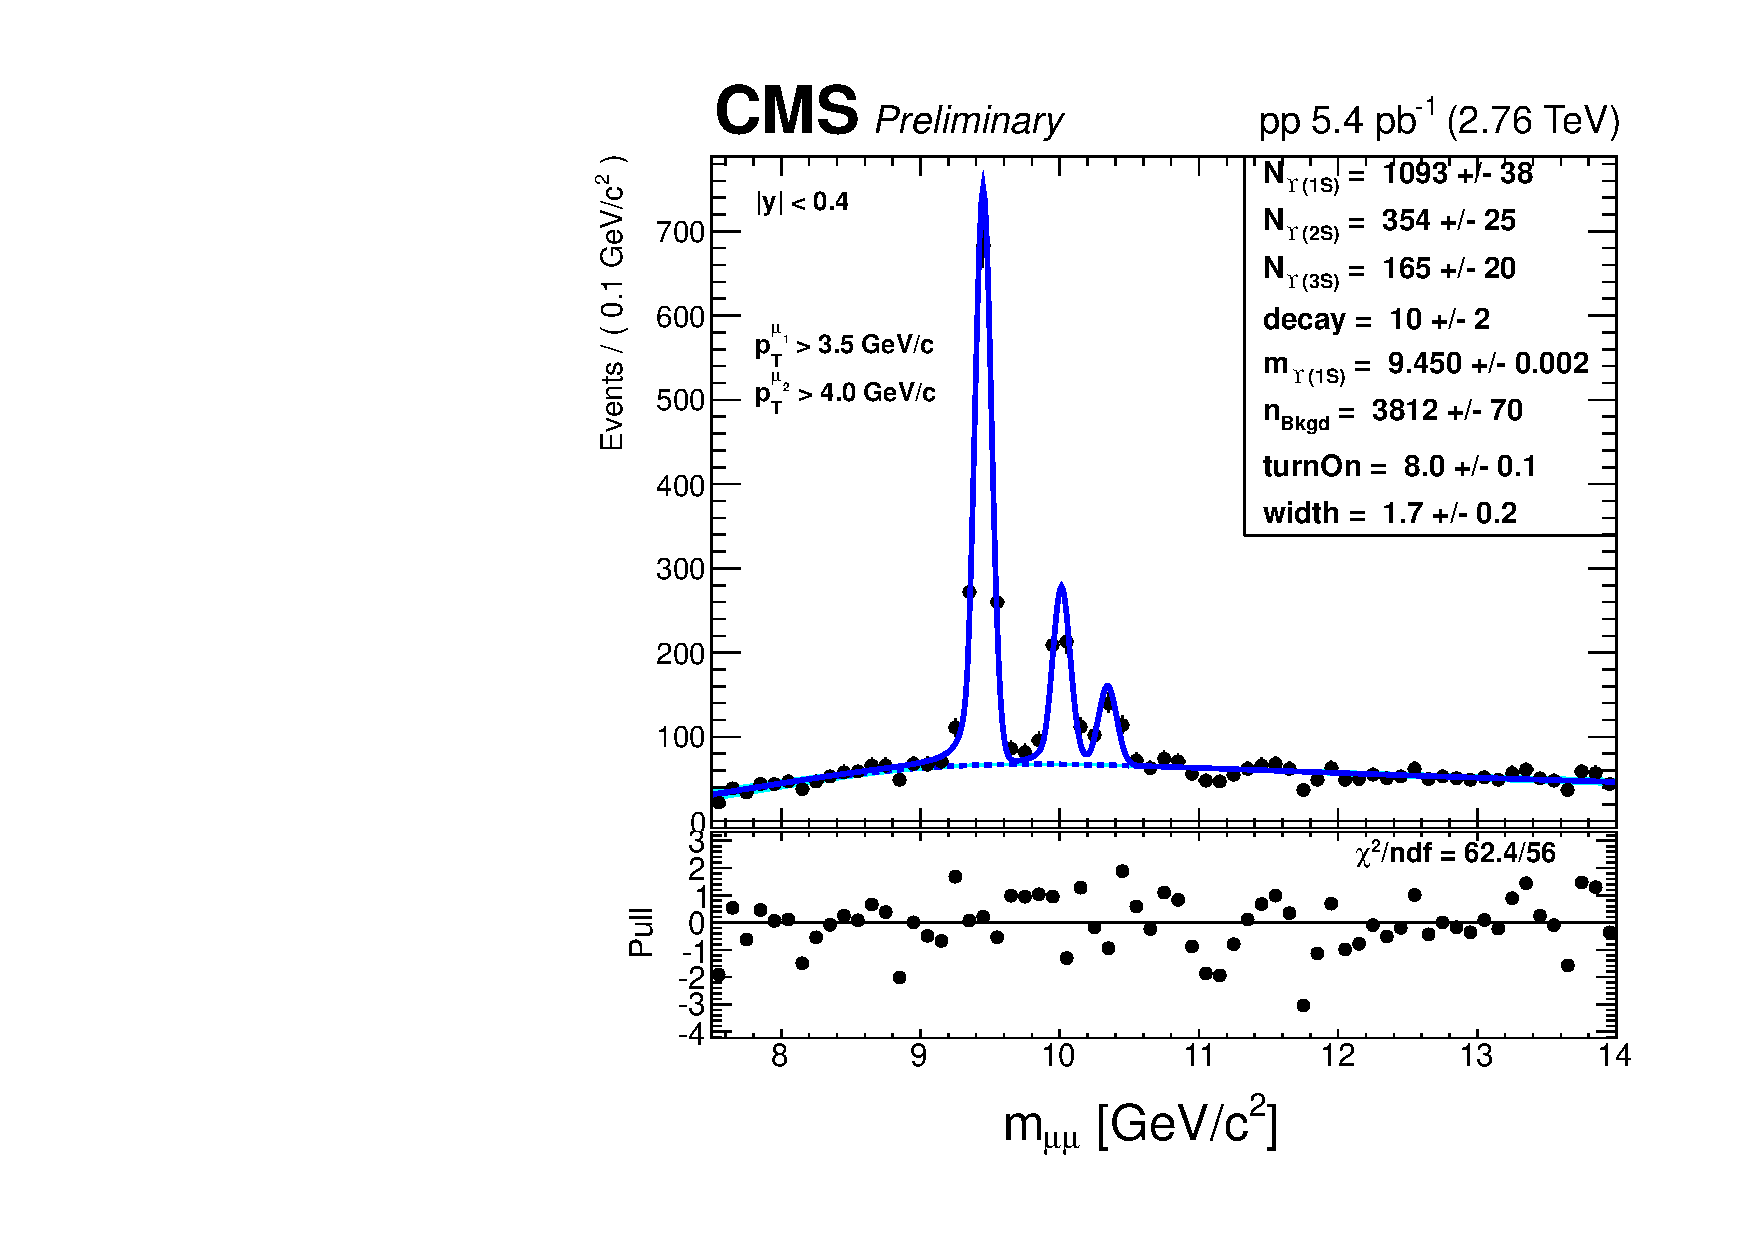
\includegraphics[width=0.49\textwidth]{Chapters/aYield/pp/pt_3p5_4/Rap/Rap_0_0p4/pp2p76tev_Rap_0_0p4_fsr1.pdf}
  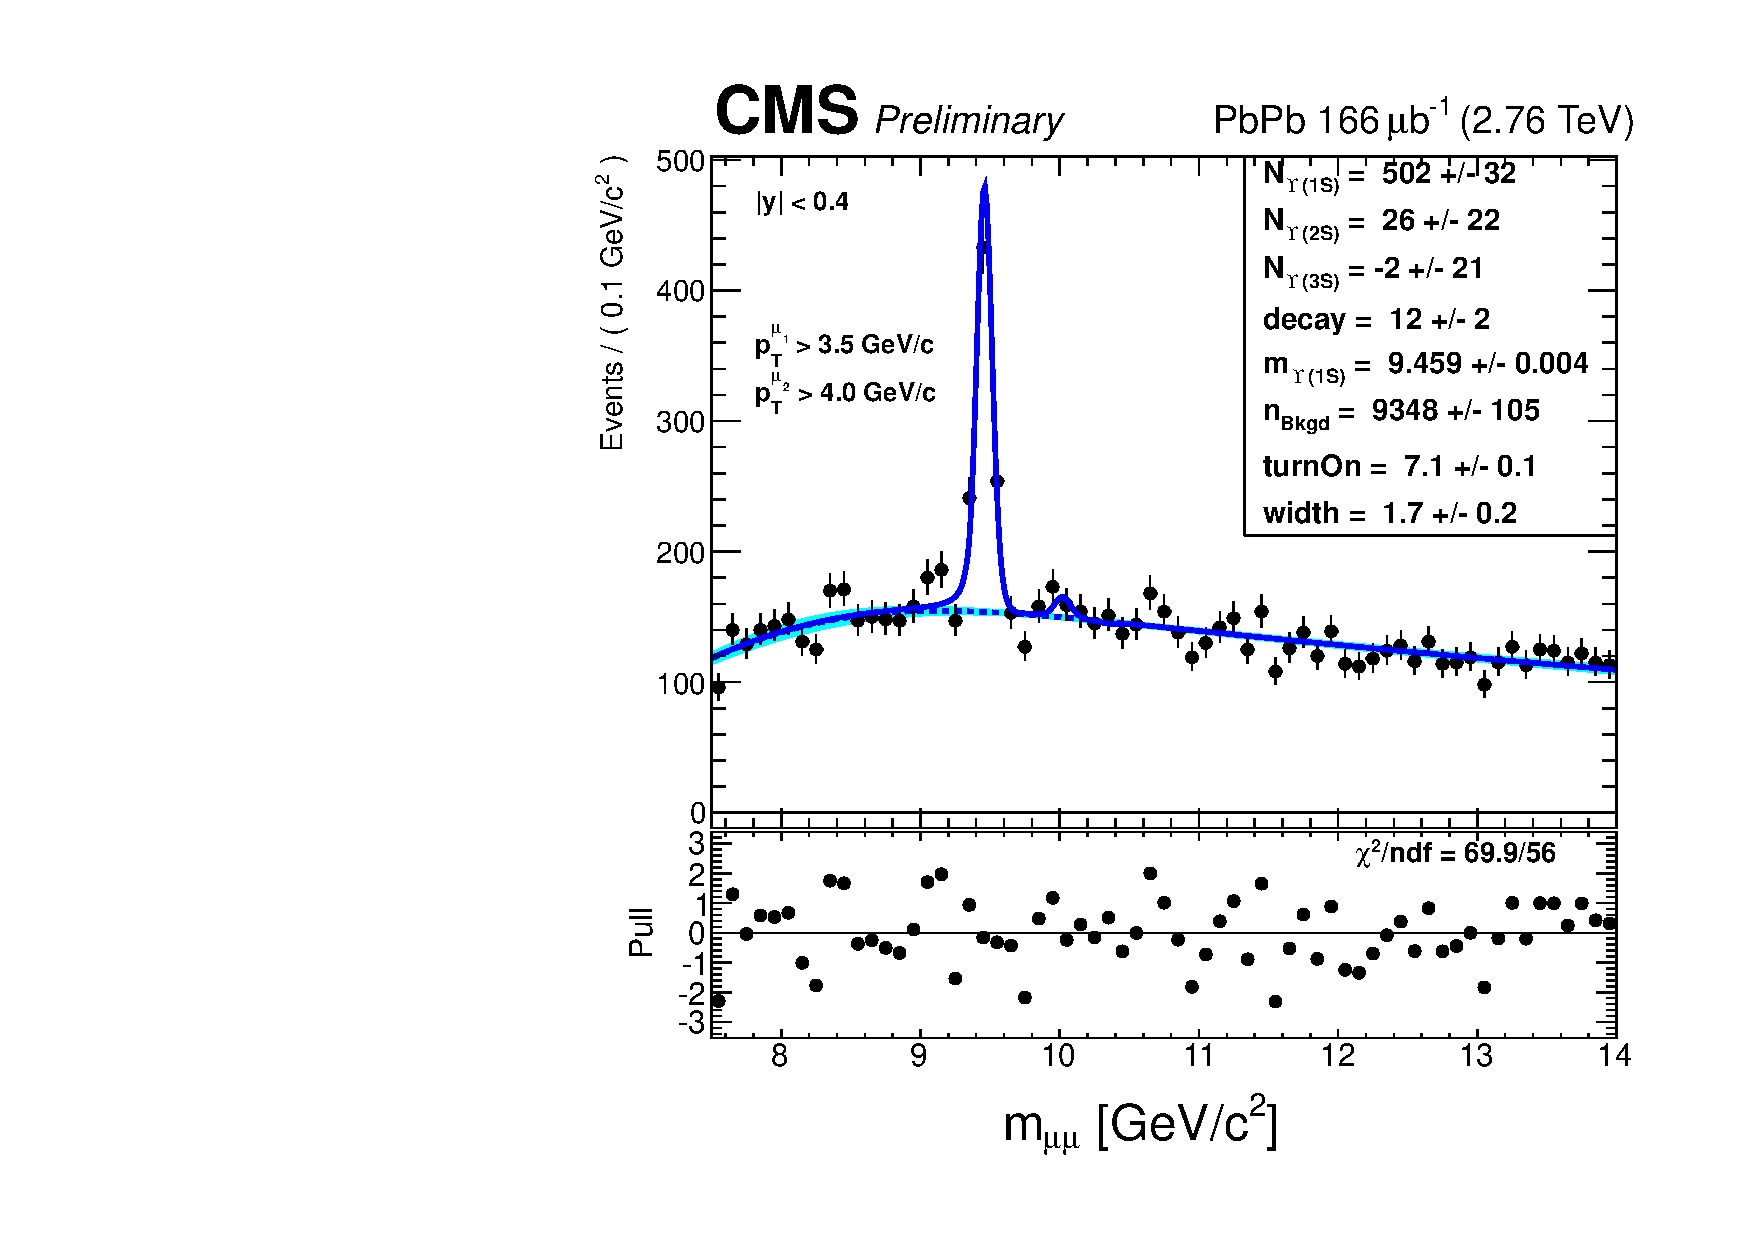
\includegraphics[width=0.49\textwidth]{Chapters/aYield/PbPb/pt_3p5_4/Rap/Rap_0_0p4/PbPb_Rap_0_0p4_fsr1.pdf}
  \caption{Fits to pp (left) and PbPb (right) datasets with loose muon cuts ($\PgUa$ analysis) in the bin $y\in [0 - 0.4]$.}
  \label{fig:YieldsErfExp_y1Sa} 
\end{figure}
\begin{figure}
  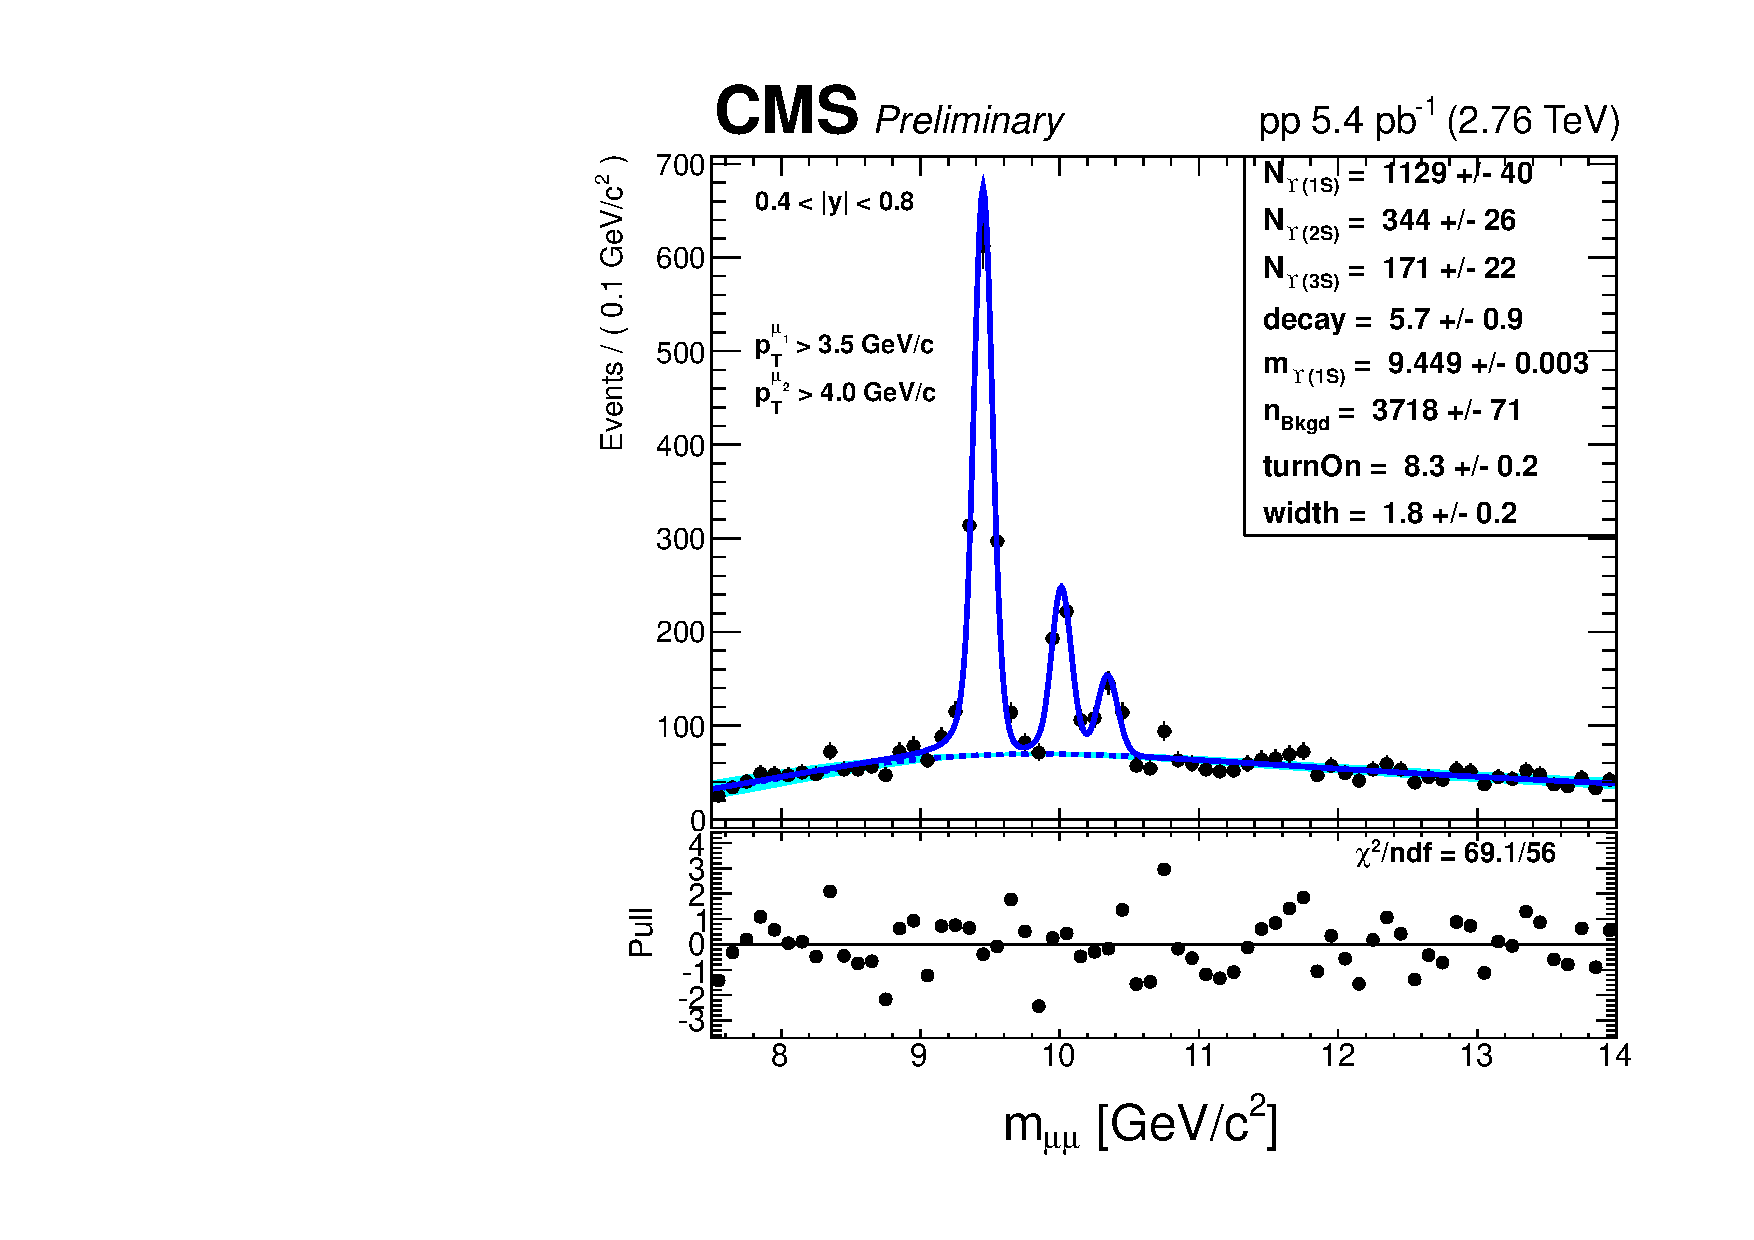
\includegraphics[width=0.49\textwidth]{Chapters/aYield/pp/pt_3p5_4/Rap/Rap_0p4_0p8/pp2p76tev_Rap_0p4_0p8_fsr1.pdf}
  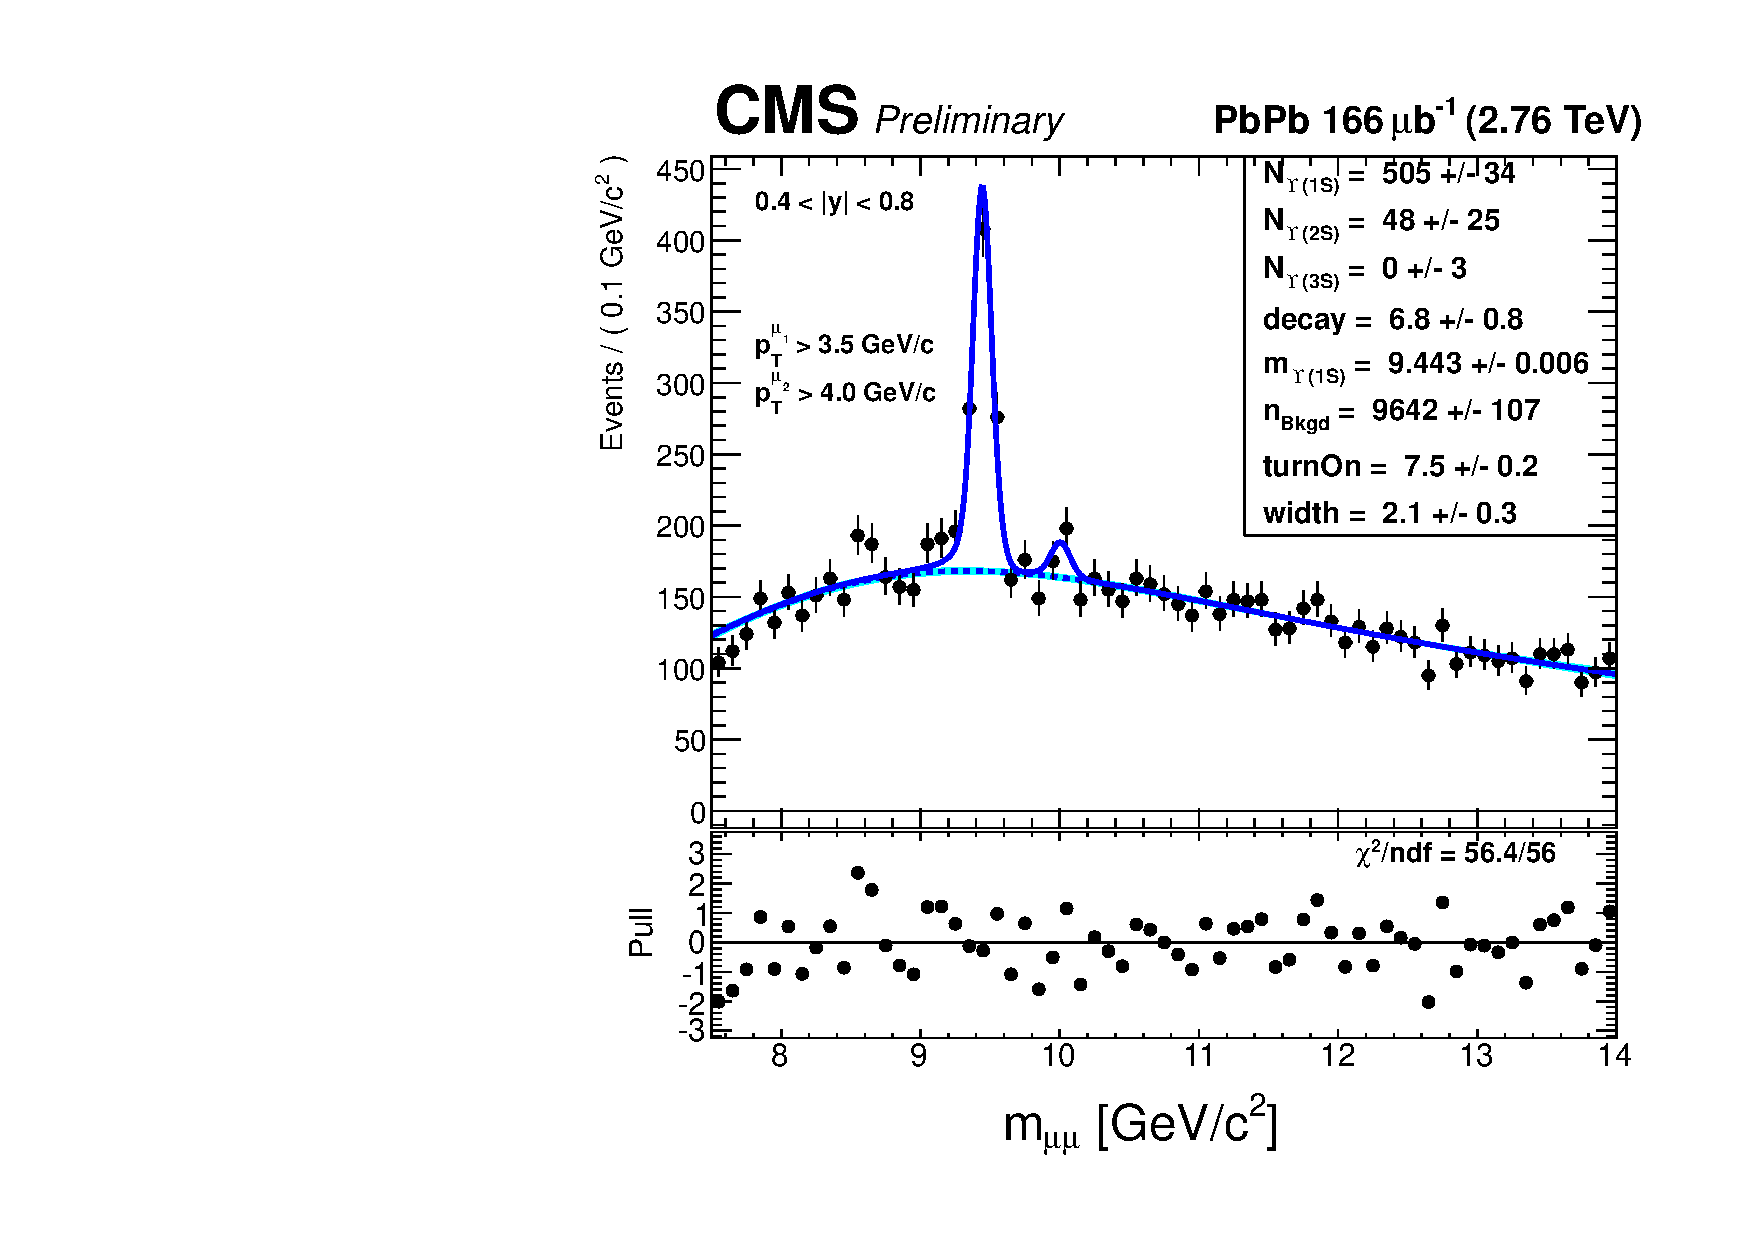
\includegraphics[width=0.49\textwidth]{Chapters/aYield/PbPb/pt_3p5_4/Rap/Rap_0p4_0p8/PbPb_Rap_0p4_0p8_fsr1.pdf} 
  \caption{Same as Figure~\ref{fig:YieldsErfExp_y1Sa} in the bin $y\in [0.4 - 0.8]$.}
  \label{fig:YieldsErfExp_y1Sb} 
\end{figure}

\begin{figure}
  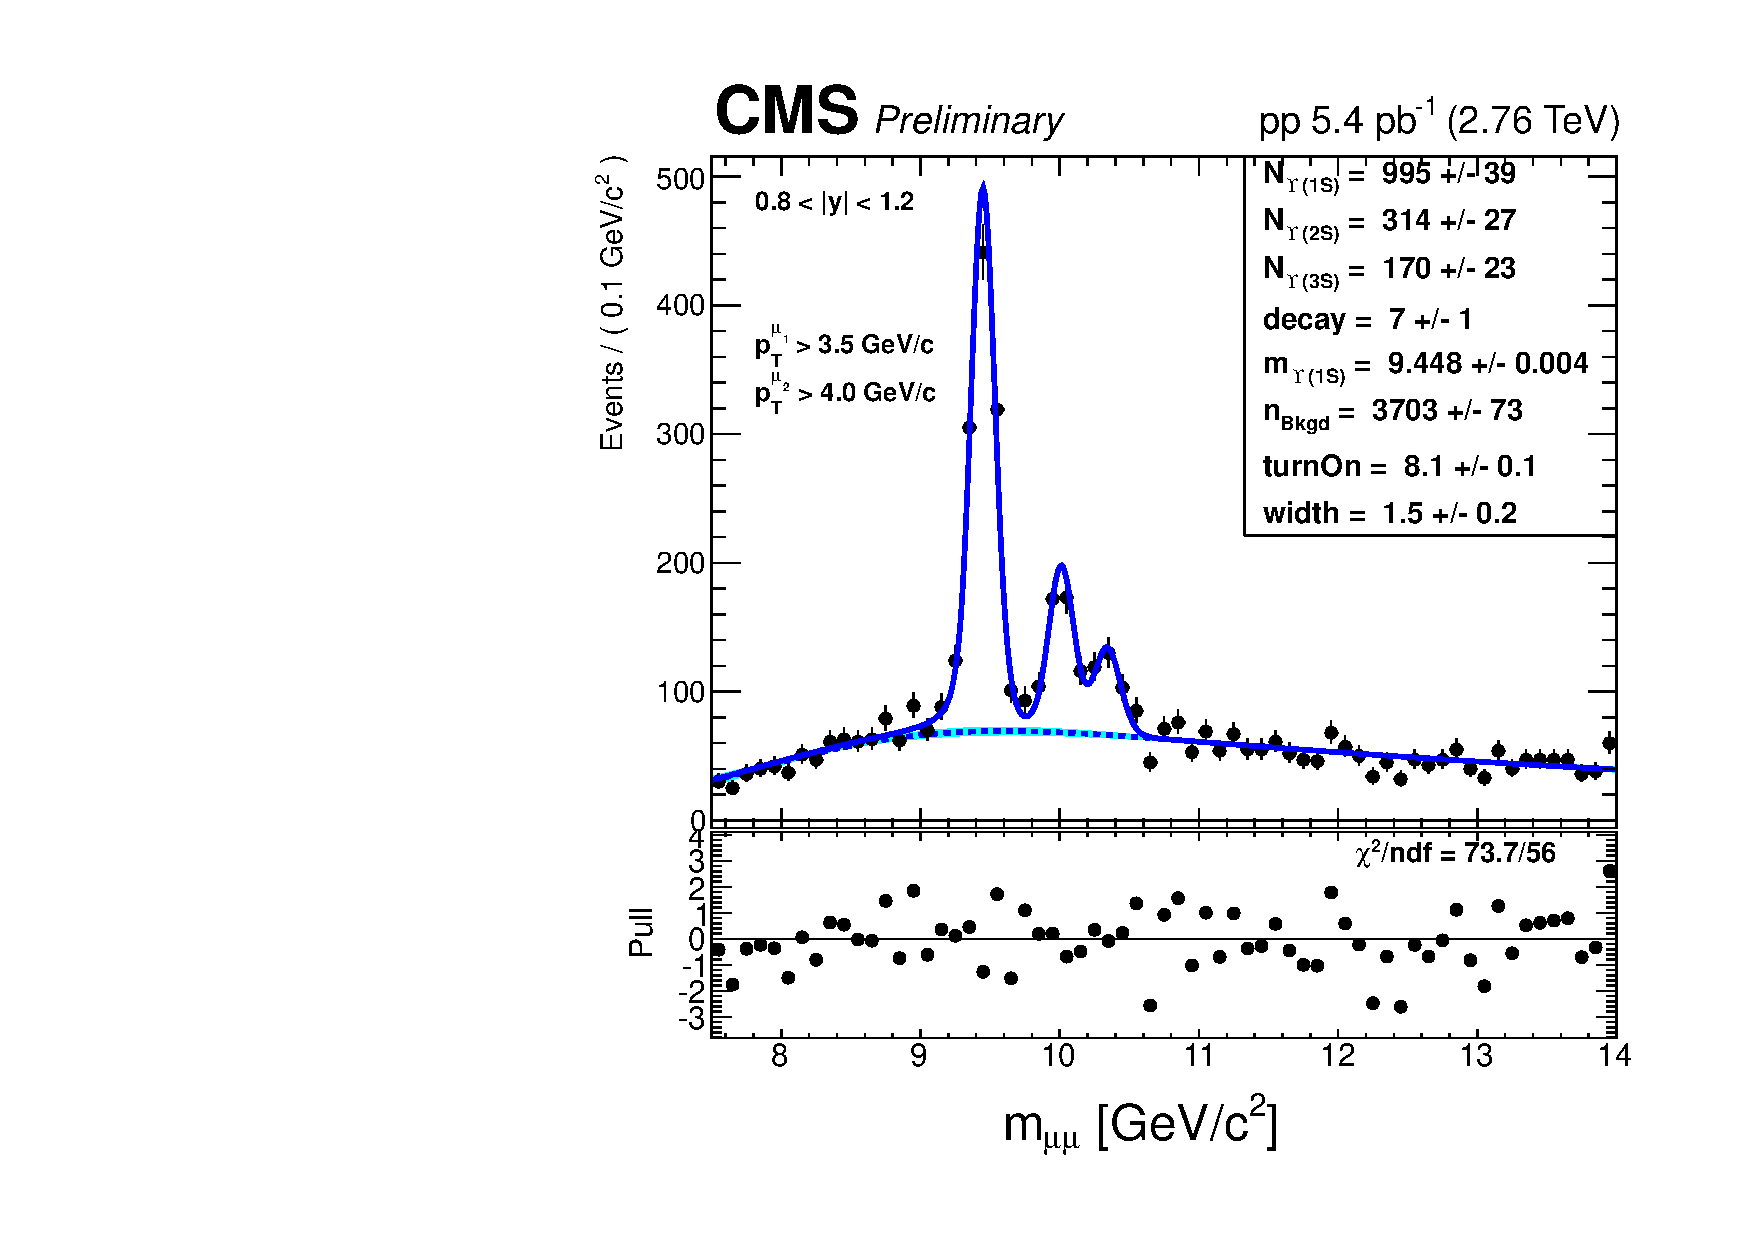
\includegraphics[width=0.49\textwidth]{Chapters/aYield/pp/pt_3p5_4/Rap/Rap_0p8_1p2/pp2p76tev_Rap_0p8_1p2_fsr1.pdf}
  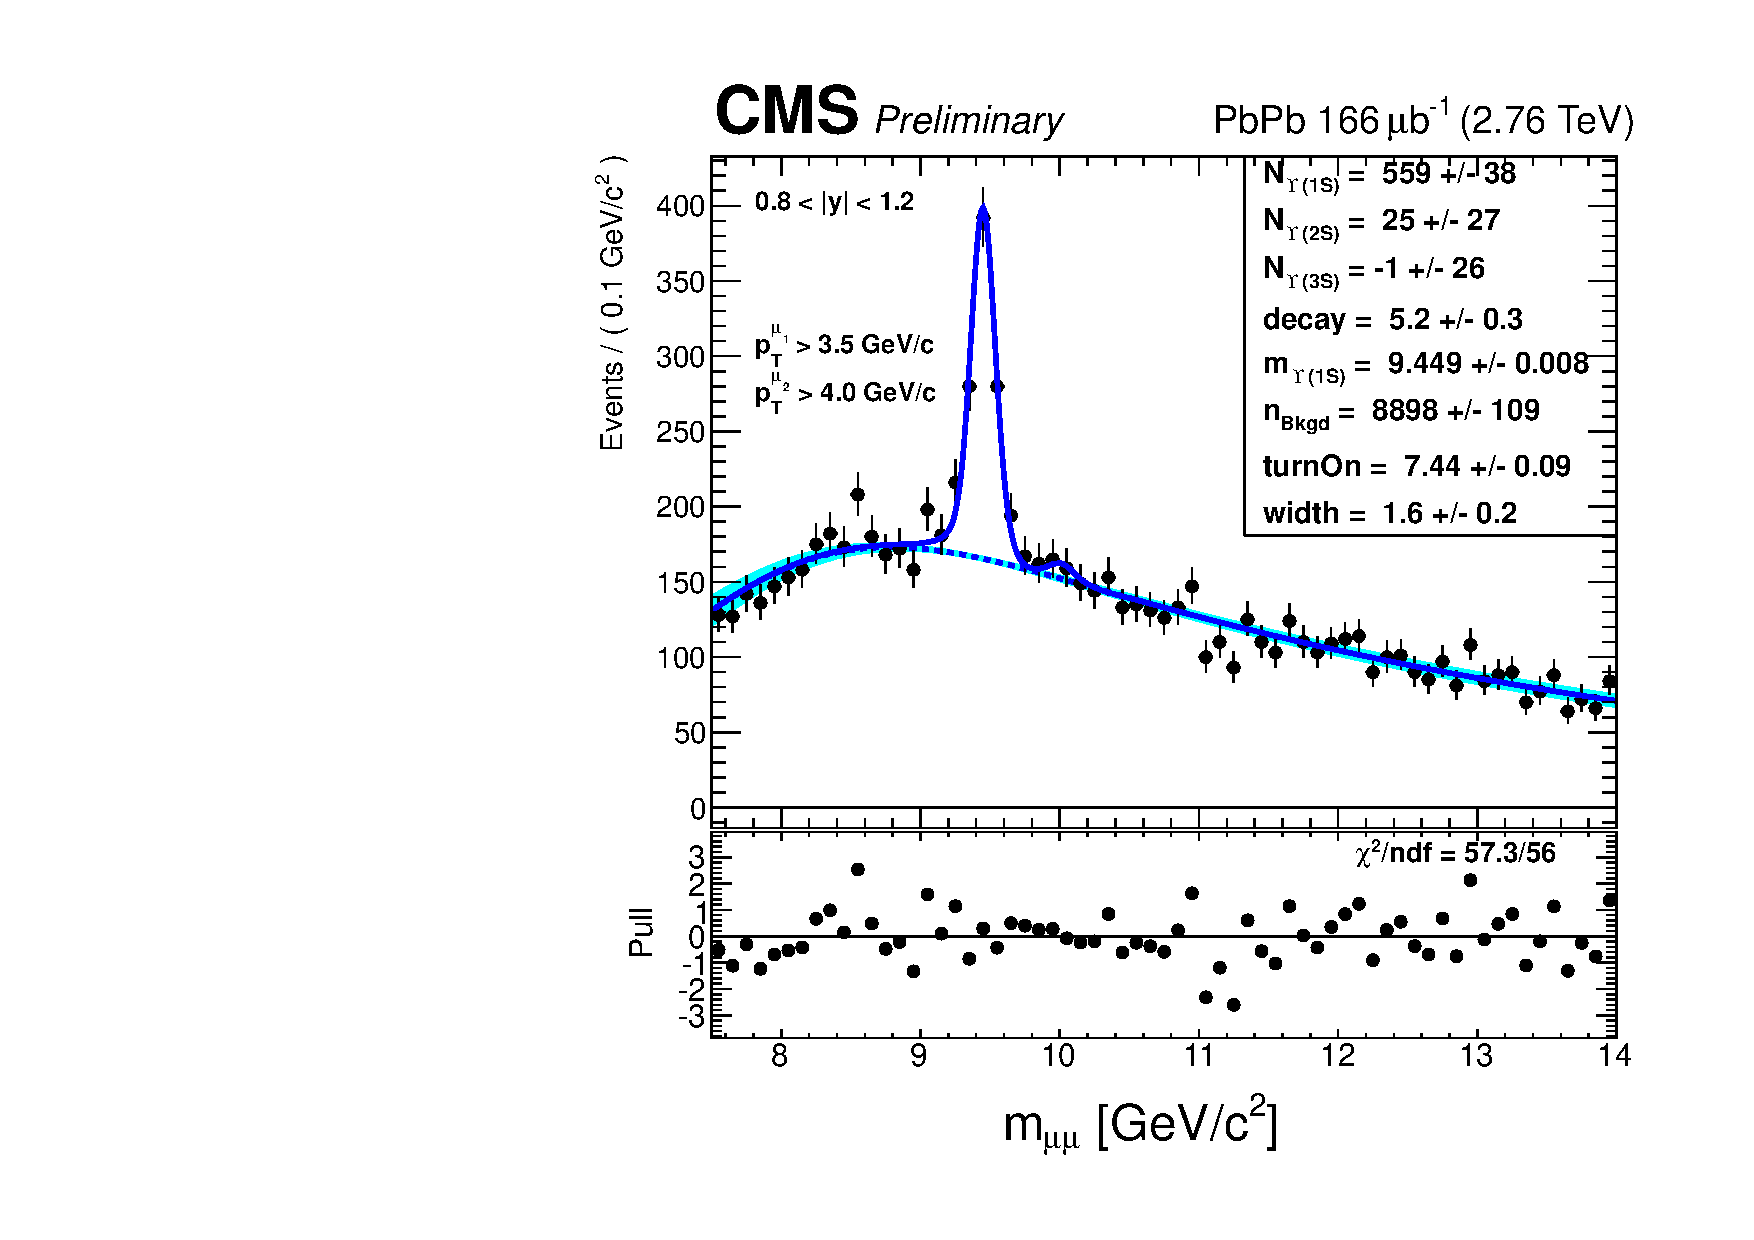
\includegraphics[width=0.49\textwidth]{Chapters/aYield/PbPb/pt_3p5_4/Rap/Rap_0p8_1p2/PbPb_Rap_0p8_1p2_fsr1.pdf}  
 \caption{Same as Figure~\ref{fig:YieldsErfExp_y1Sa} in the bin $y\in [0.8 - 1.2]$.}
  \label{fig:YieldsErfExp_y1Sc} 
\end{figure}

\begin{figure}
  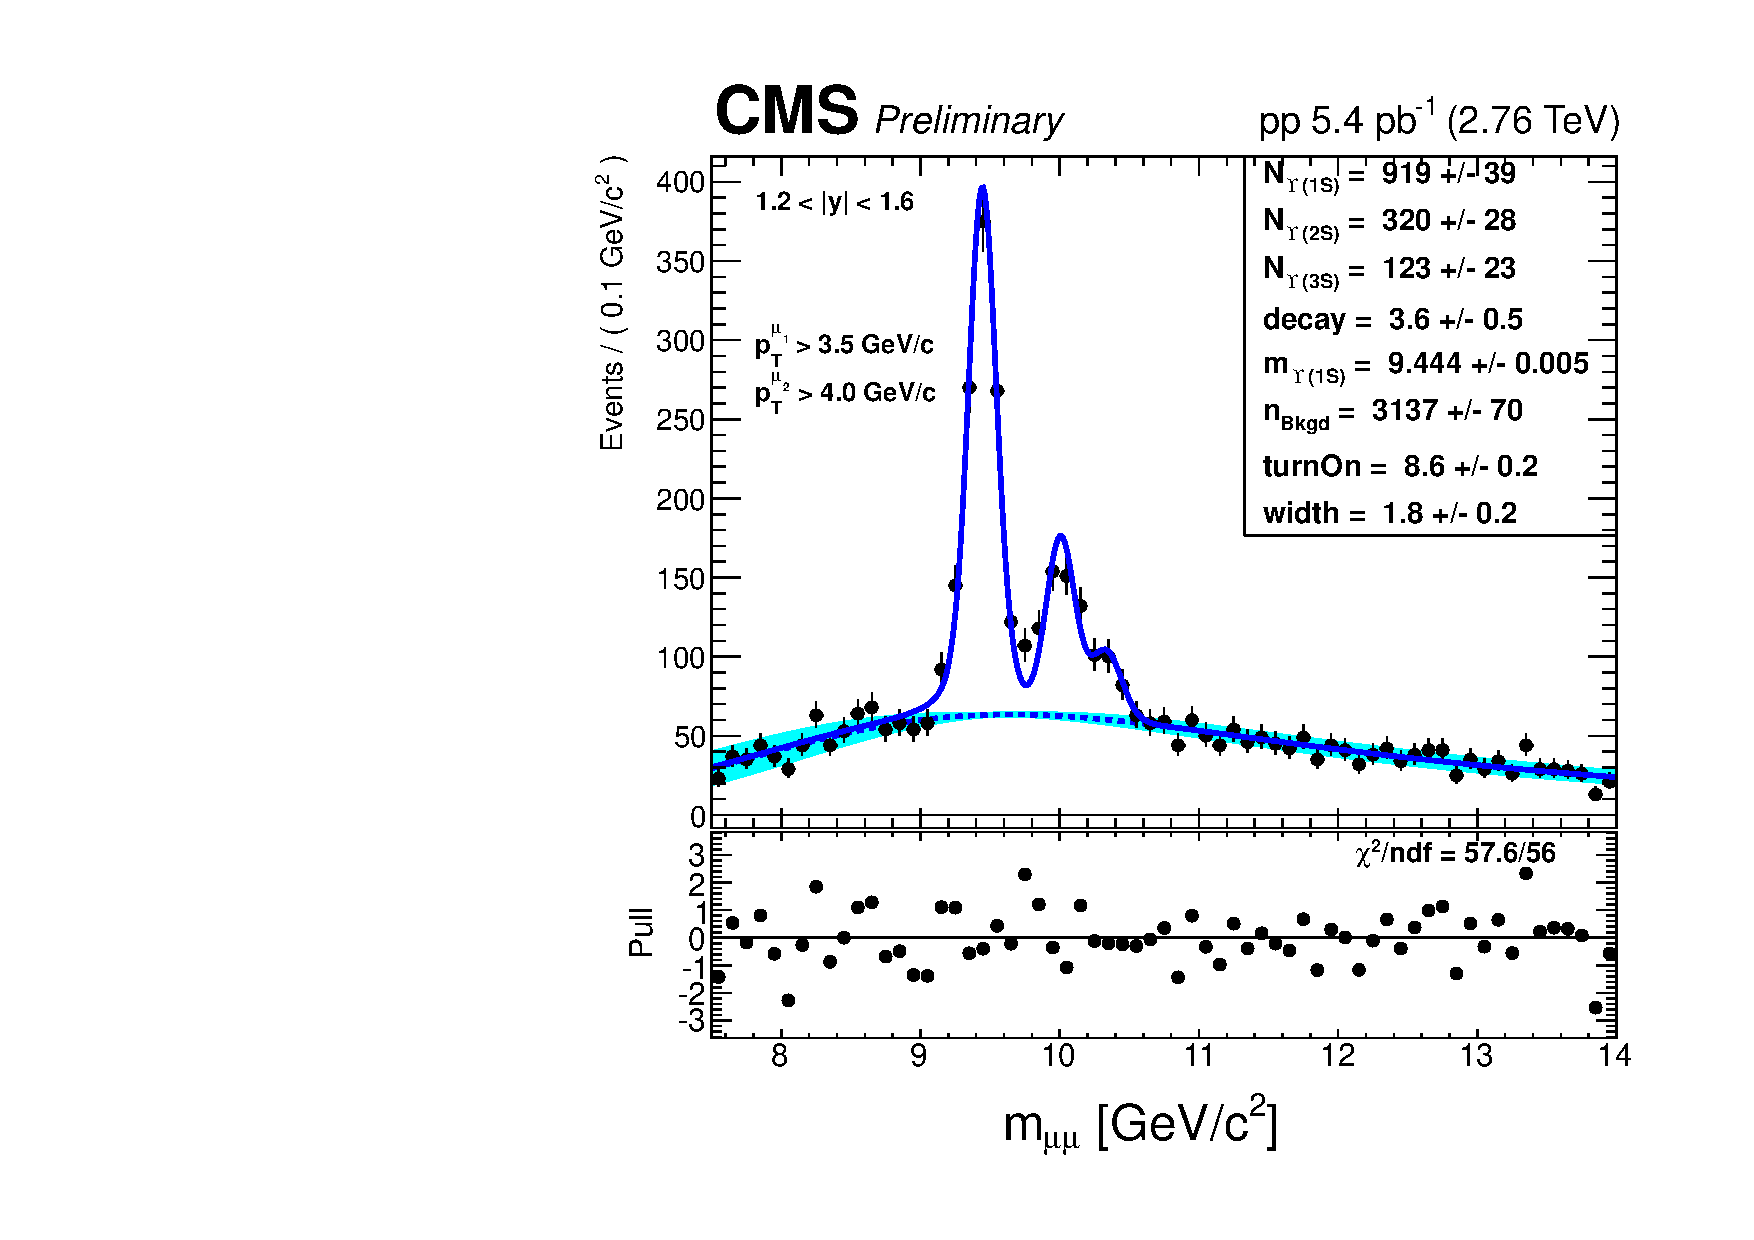
\includegraphics[width=0.49\textwidth]{Chapters/aYield/pp/pt_3p5_4/Rap/Rap_1p2_1p6/pp2p76tev_Rap_1p2_1p6_fsr1.pdf}
  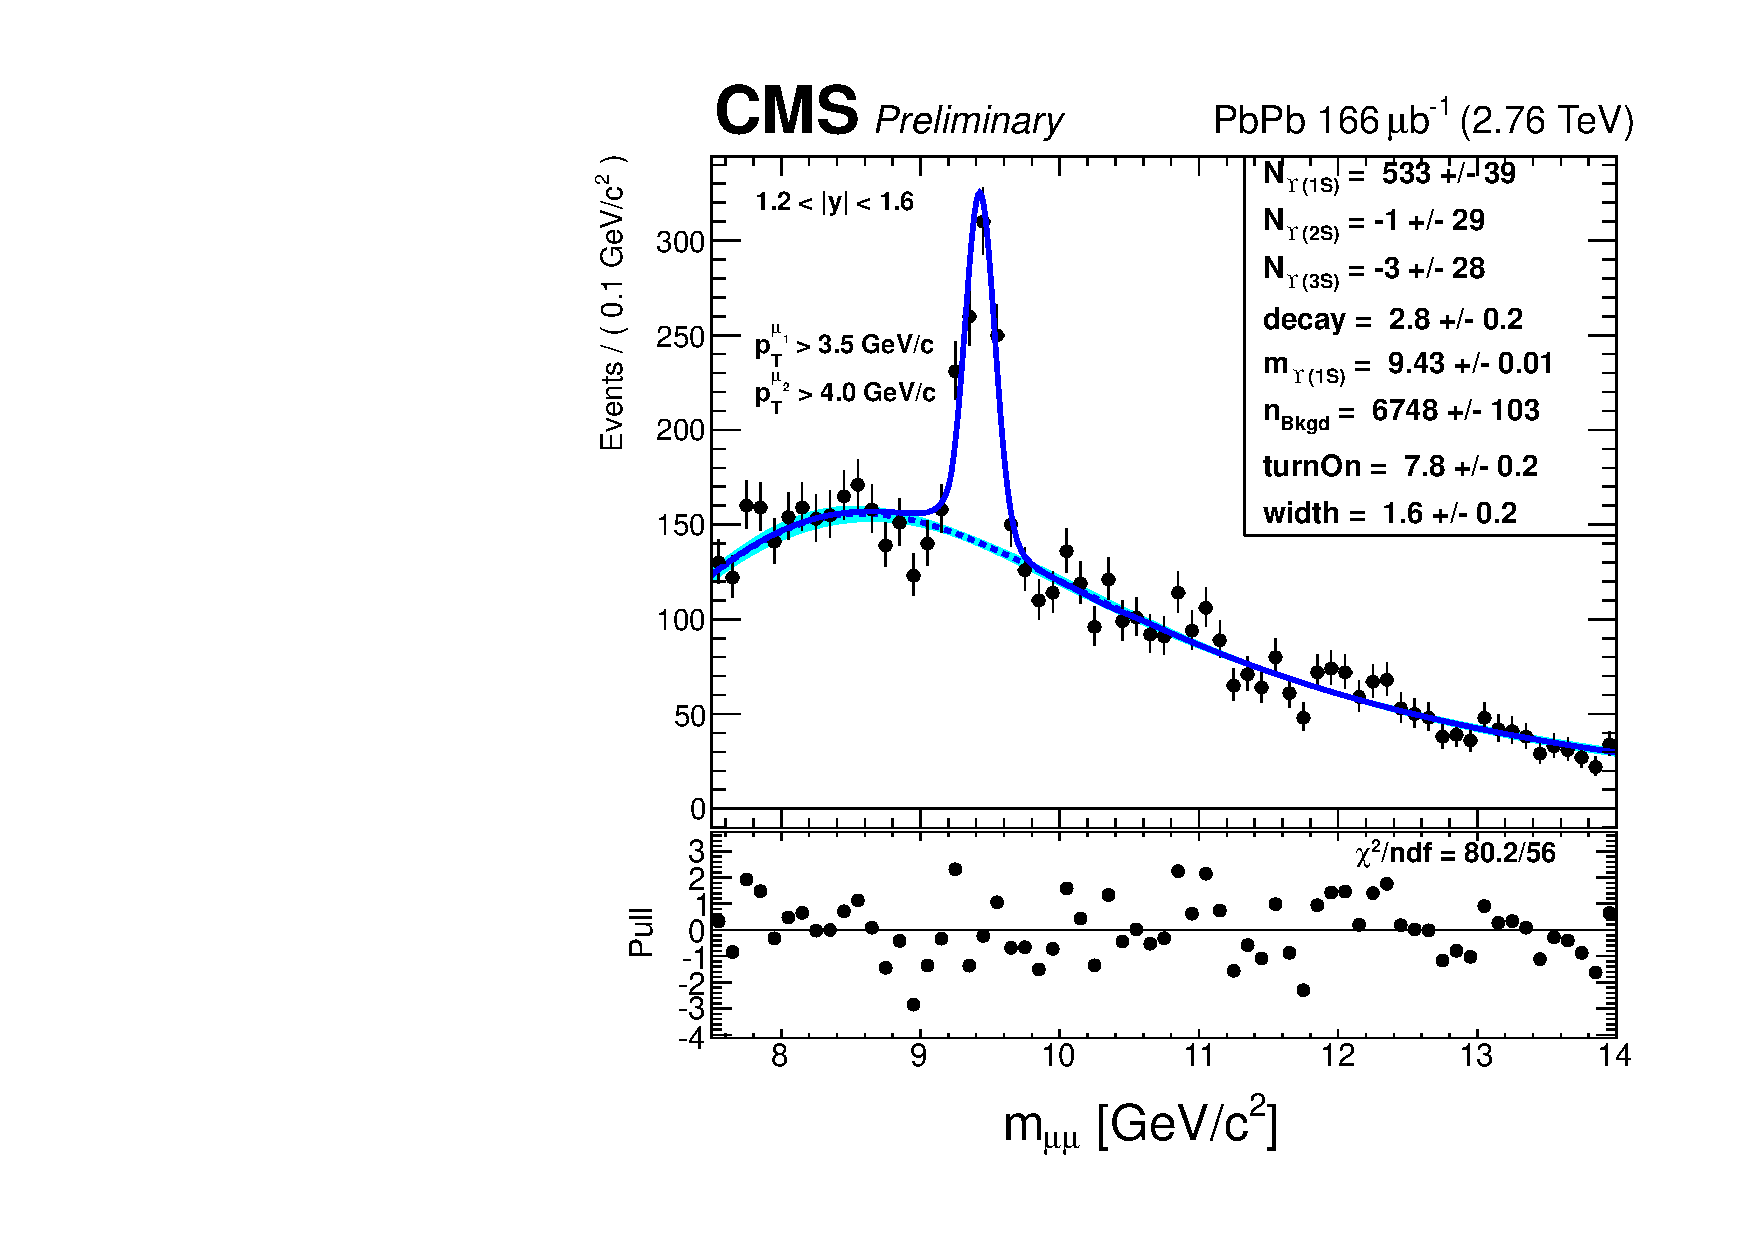
\includegraphics[width=0.49\textwidth]{Chapters/aYield/PbPb/pt_3p5_4/Rap/Rap_1p2_1p6/PbPb_Rap_1p2_1p6_fsr1.pdf}  
 \caption{Same as Figure~\ref{fig:YieldsErfExp_y1Sa} in the bin $y\in [1.2 - 1.6]$.}
  \label{fig:YieldsErfExp_y1Sd} 
\end{figure}
\begin{figure}
  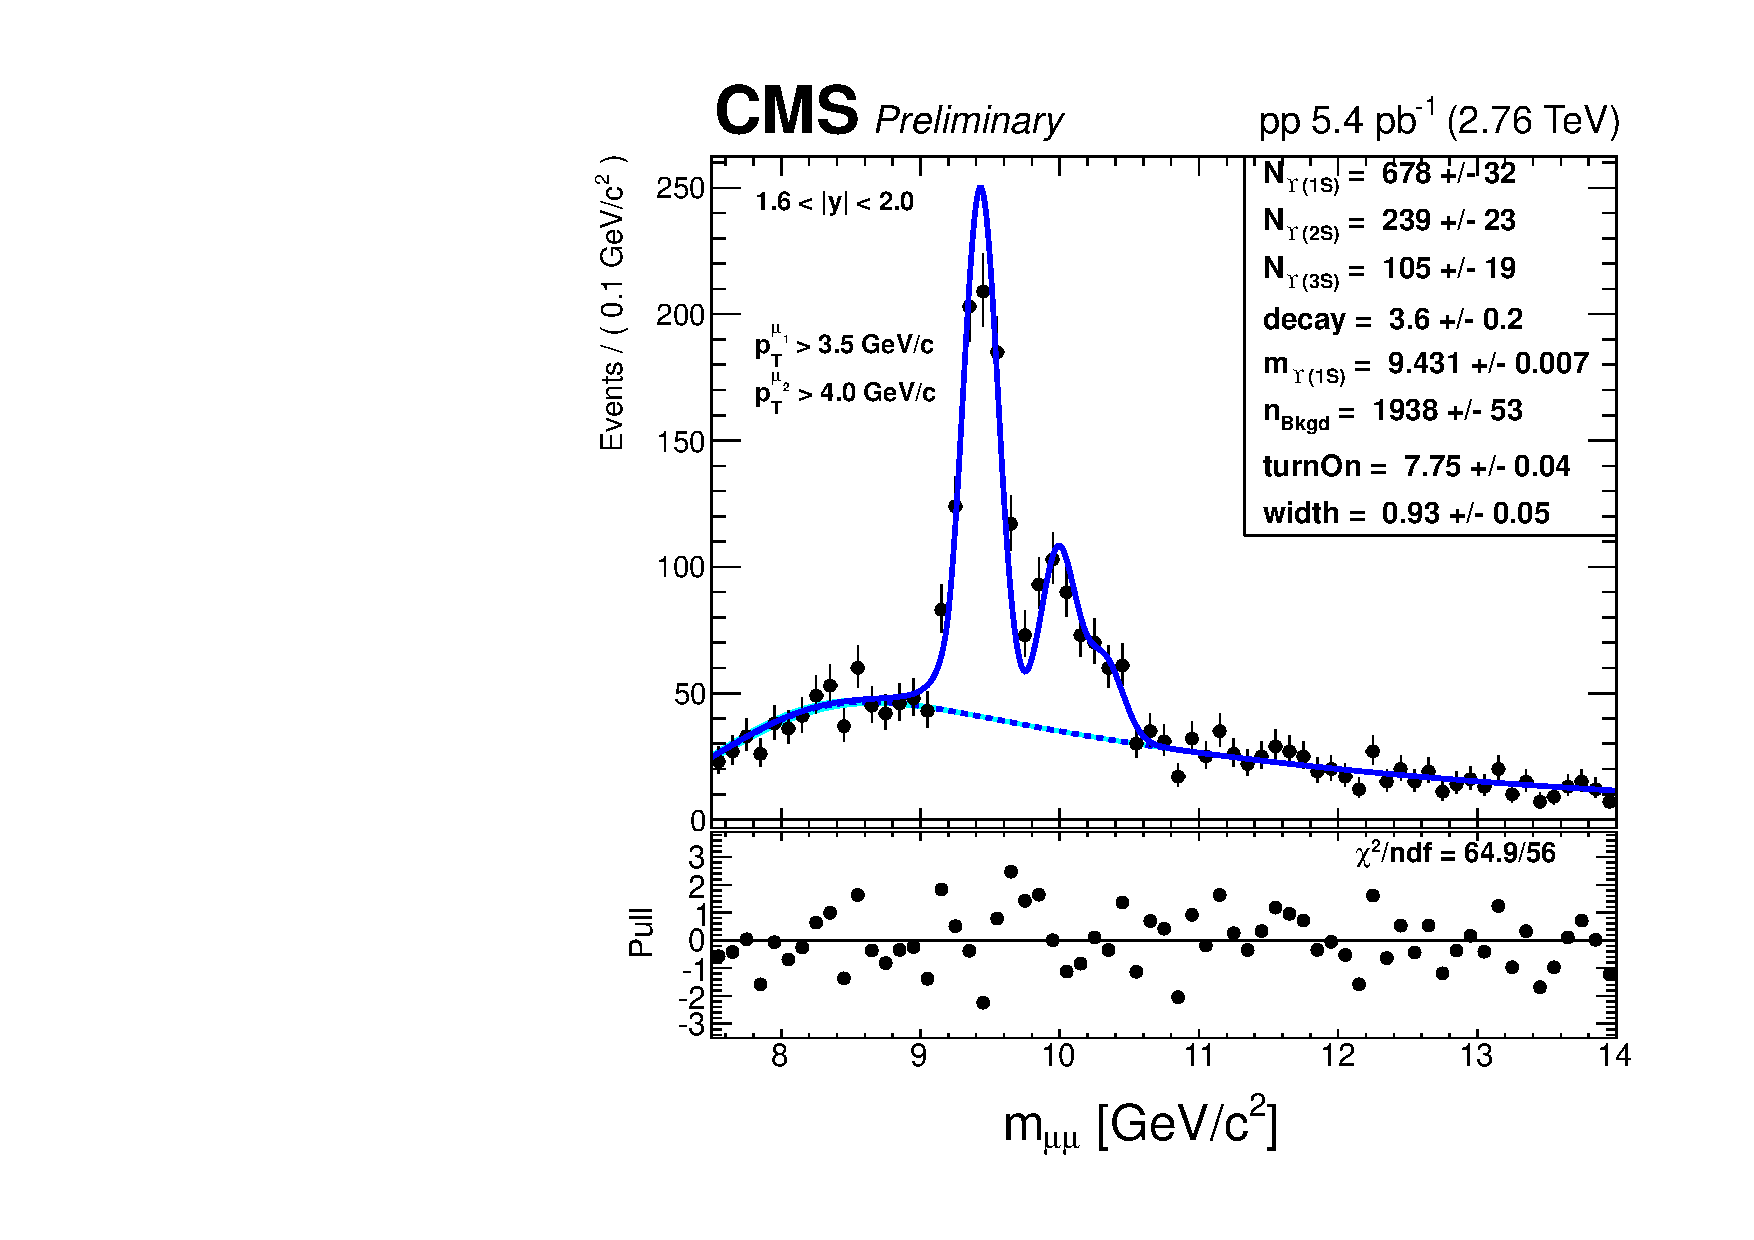
\includegraphics[width=0.49\textwidth]{Chapters/aYield/pp/pt_3p5_4/Rap/Rap_1p6_2/pp2p76tev_Rap_1p6_2_fsr1.pdf}
  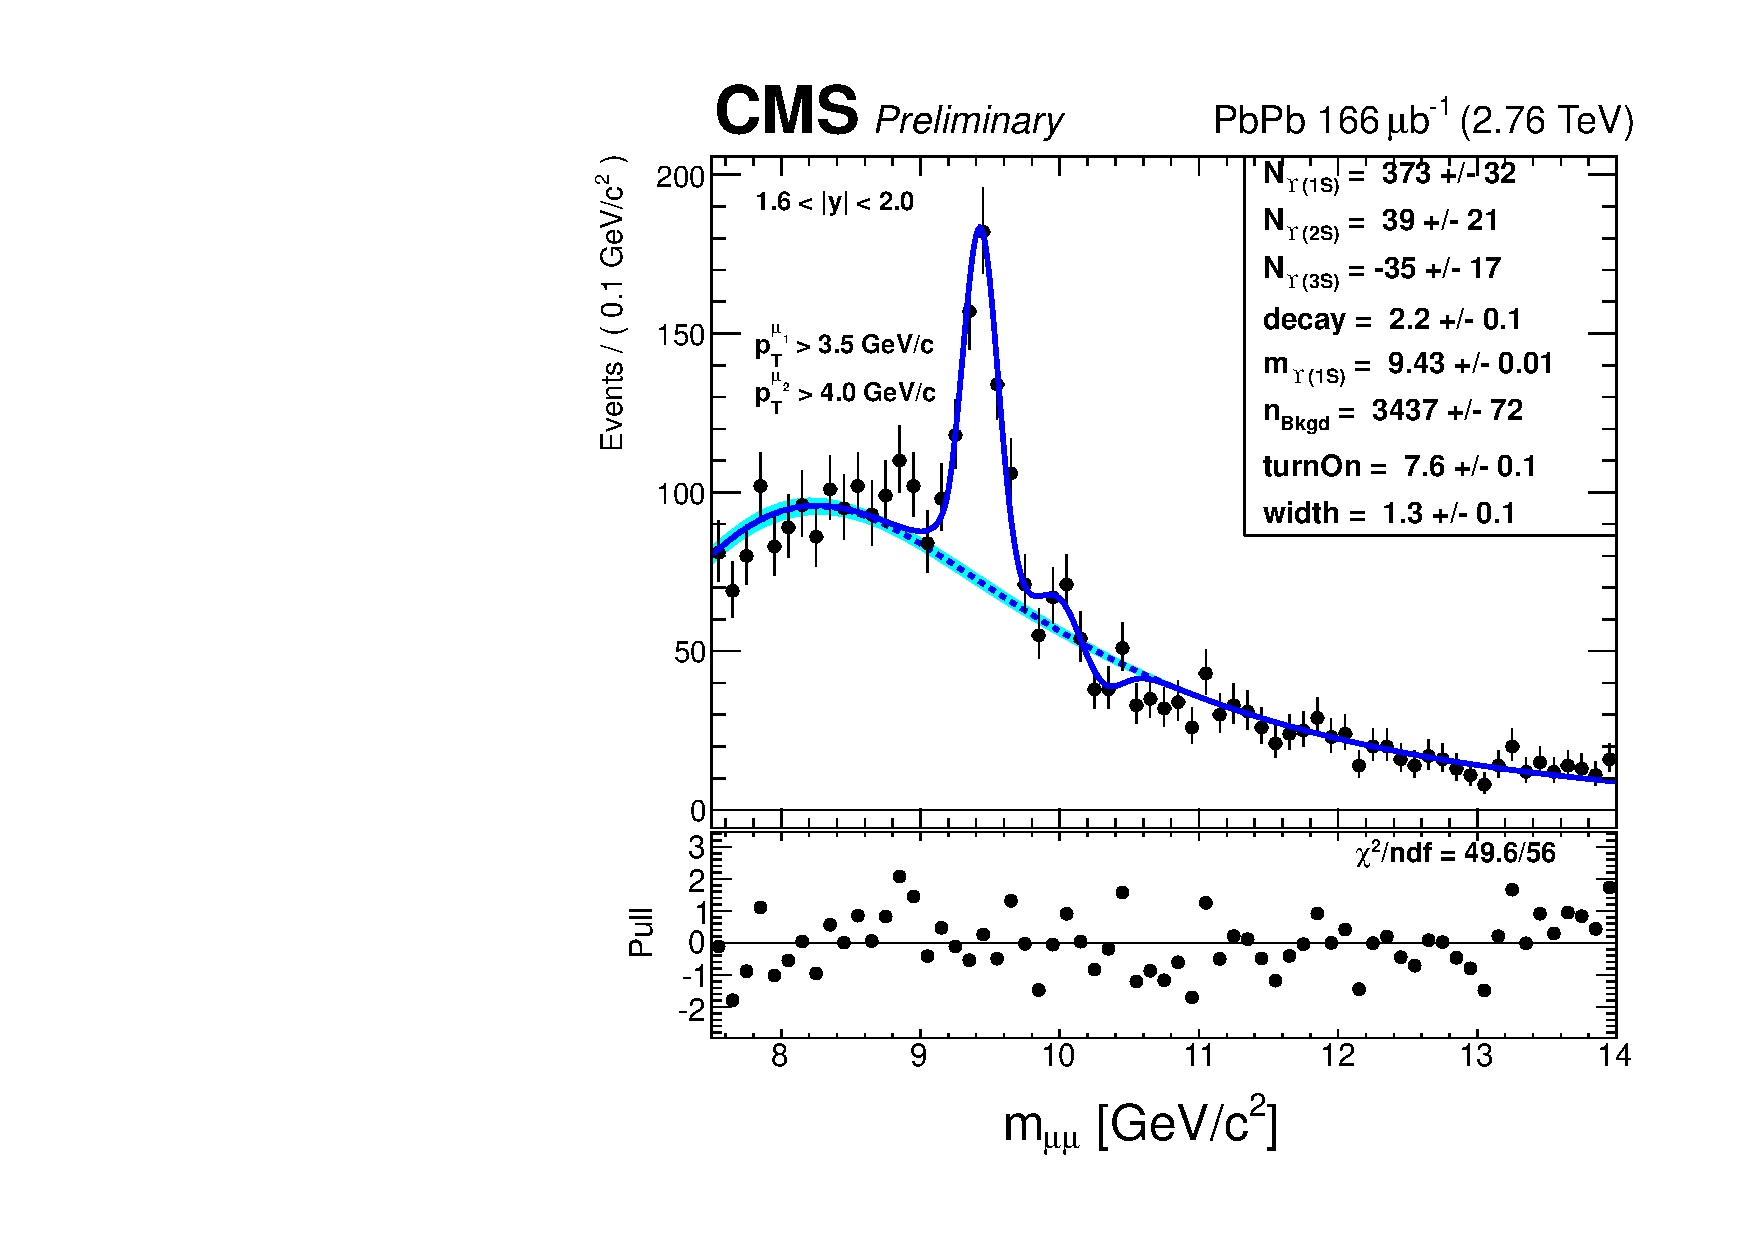
\includegraphics[width=0.49\textwidth]{Chapters/aYield/PbPb/pt_3p5_4/Rap/Rap_1p6_2/PbPb_Rap_1p6_2_fsr1.pdf}
  \caption{Same as Figure~\ref{fig:YieldsErfExp_y1Sa} in the bin $y\in [1.6 - 2]$.}
  \label{fig:YieldsErfExp_y1Se} 
\end{figure}
\begin{figure}
  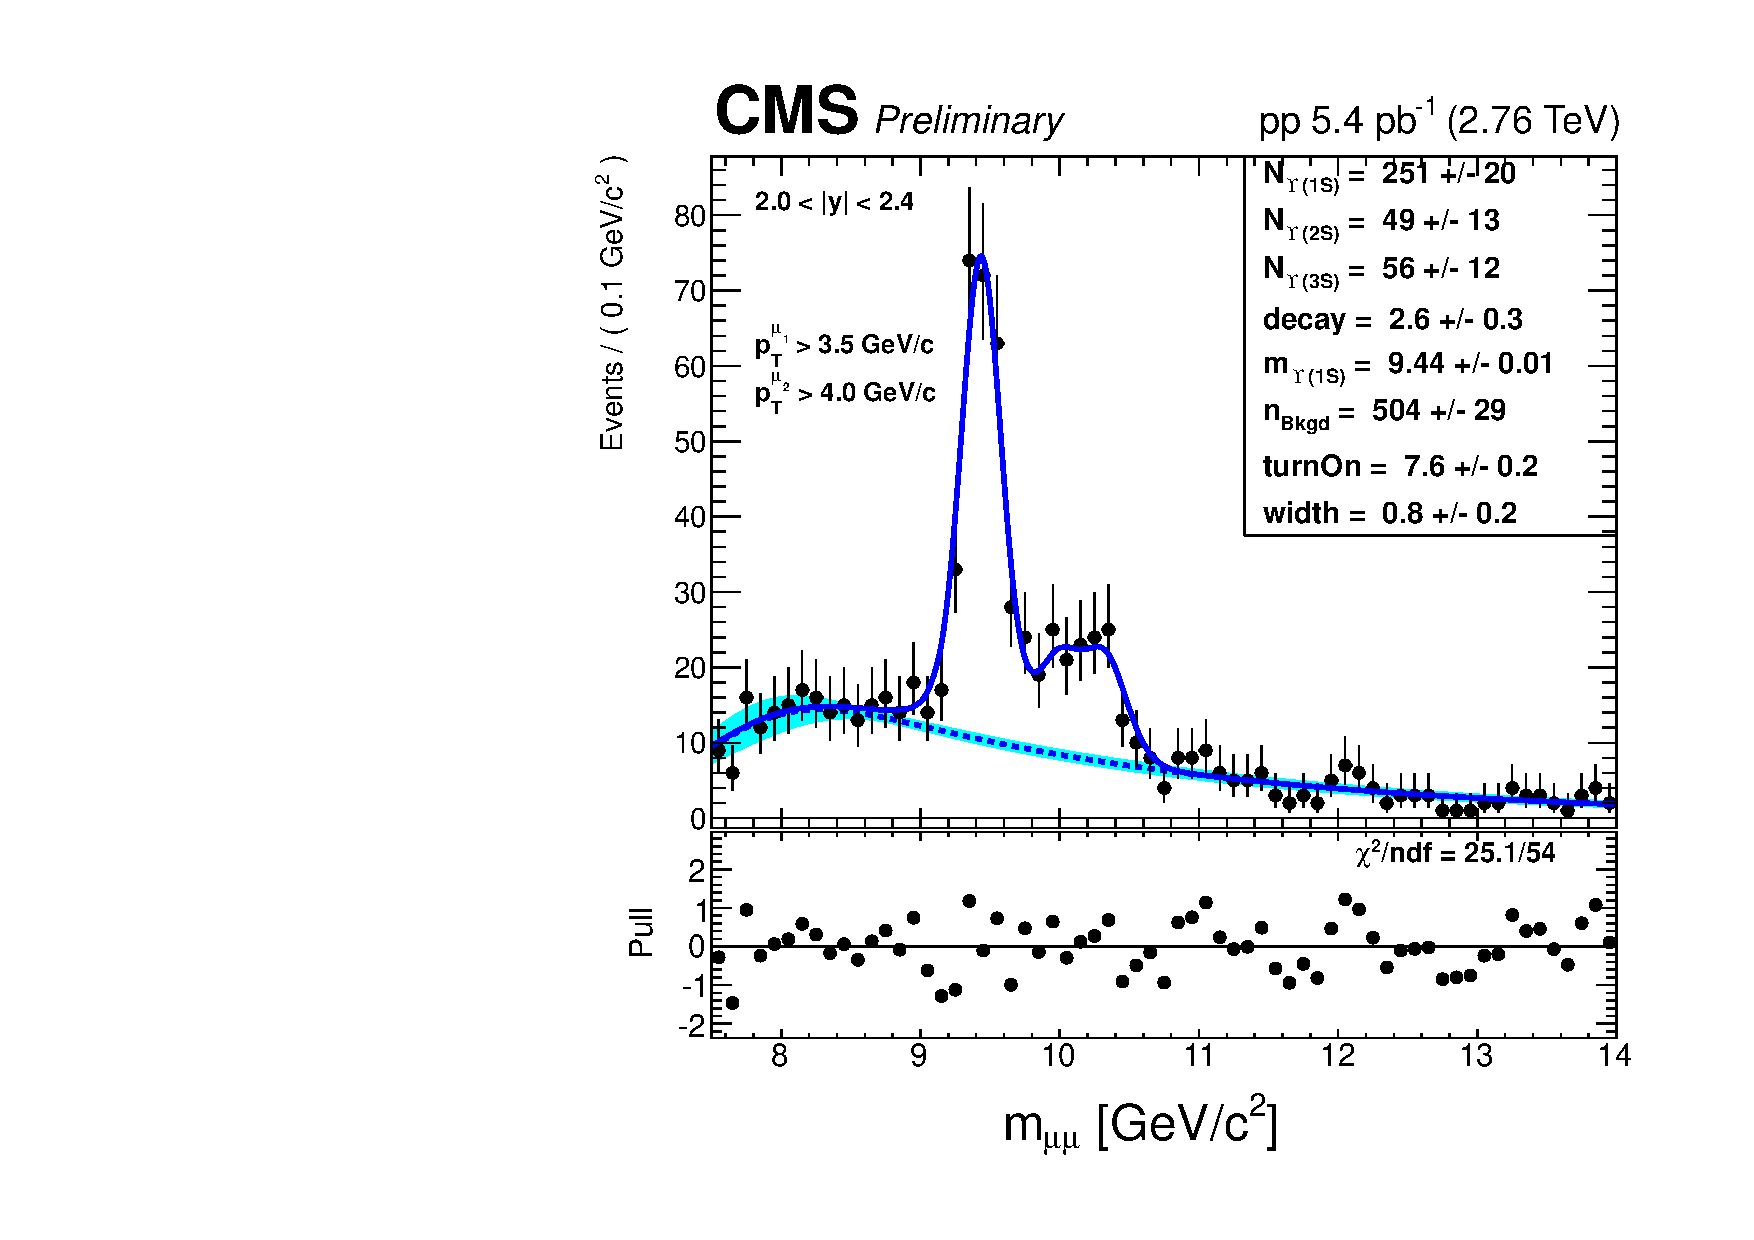
\includegraphics[width=0.49\textwidth]{Chapters/aYield/pp/pt_3p5_4/Rap/Rap_2_2p4/pp2p76tev_Rap_2_2p4_fsr1.pdf}
  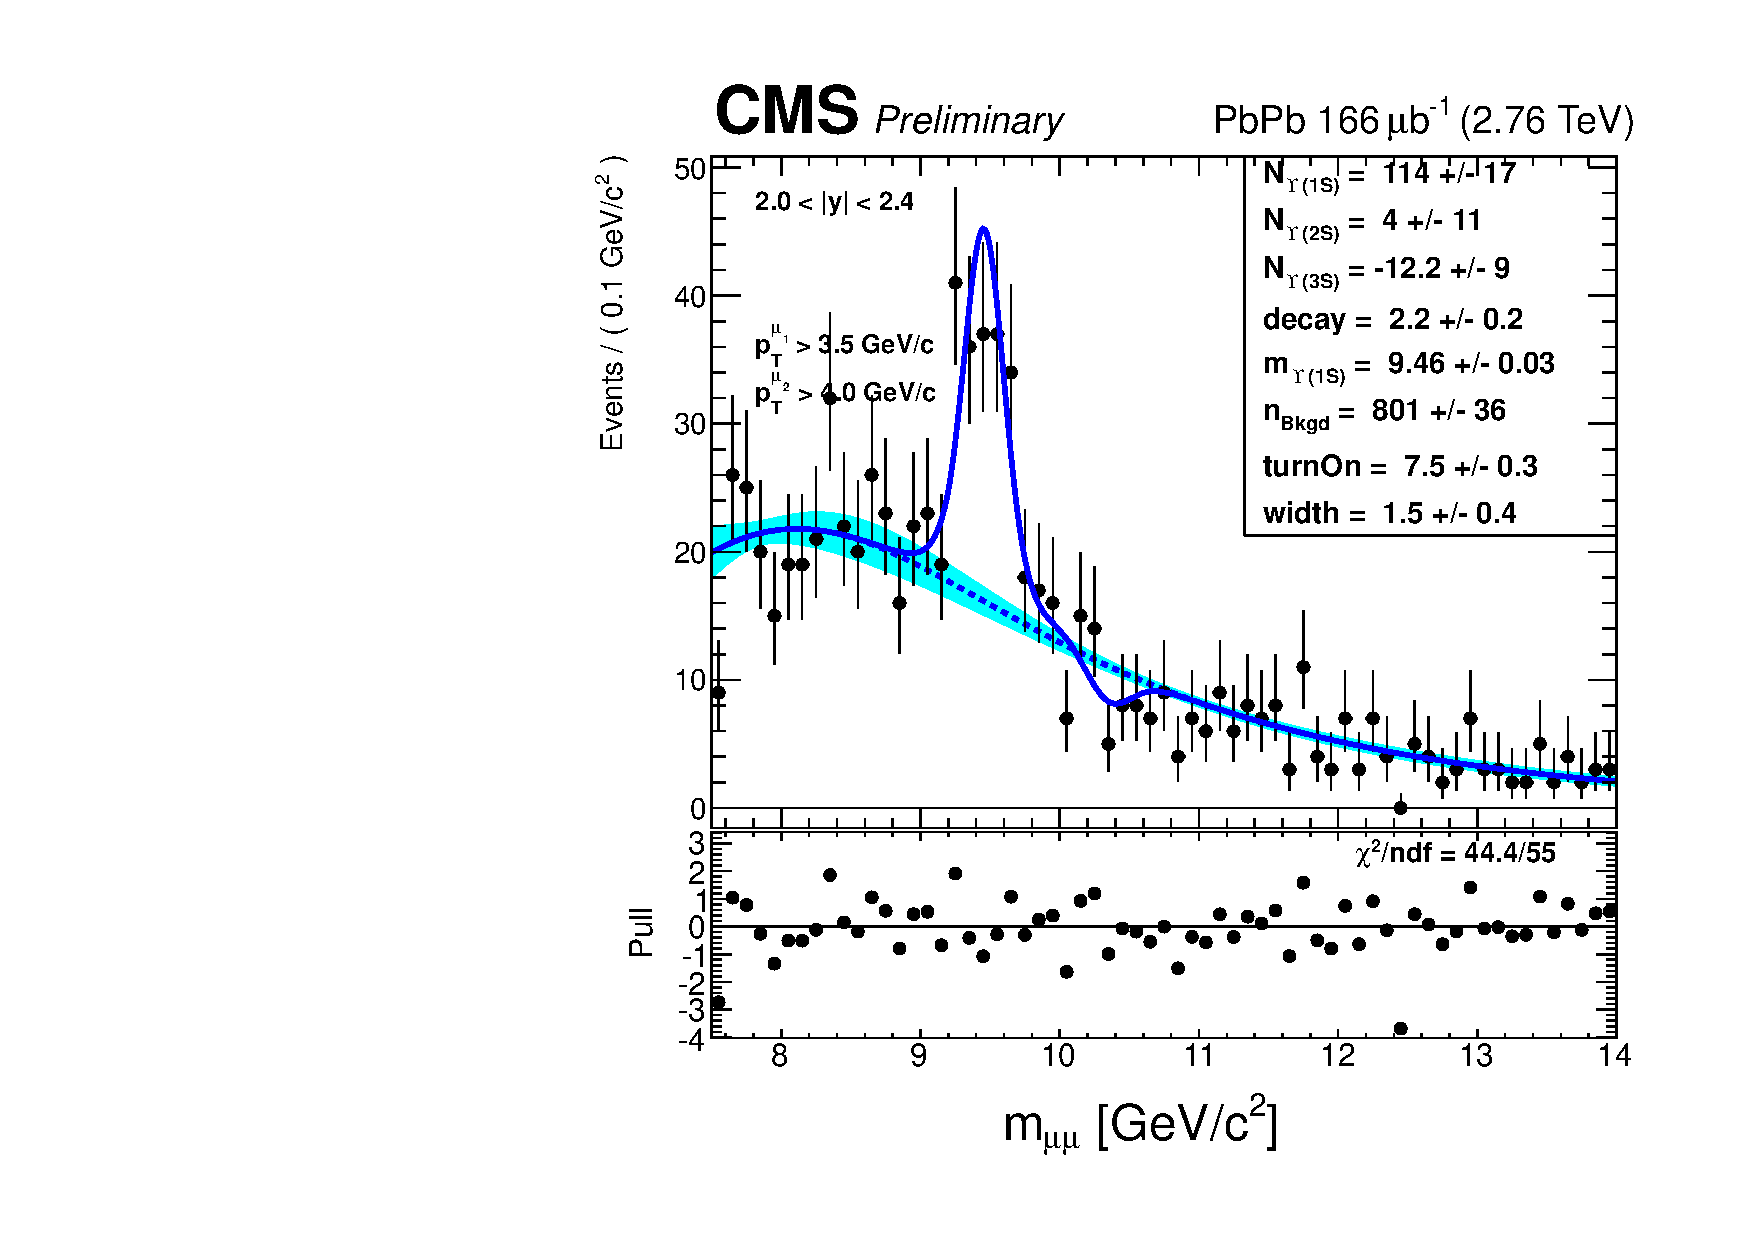
\includegraphics[width=0.49\textwidth]{Chapters/aYield/PbPb/pt_3p5_4/Rap/Rap_2_2p4/PbPb_Rap_2_2p4_fsr1.pdf}
  \caption{Same as Figure~\ref{fig:YieldsErfExp_y1Sa} in the bin $y\in [2 - 2.4]$.}
  \label{fig:YieldsErfExp_y1Sf} 
\end{figure}

Figure~\ref{fig:YieldsErfExp_y2Sa} and~\ref{fig:YieldsErfExp_y2Sb}
present the two rapidity bins of the \PgUb\ analysis, used in the
computation of the \RAA(\PgUb) in wide bins of rapidity.
\begin{figure}
   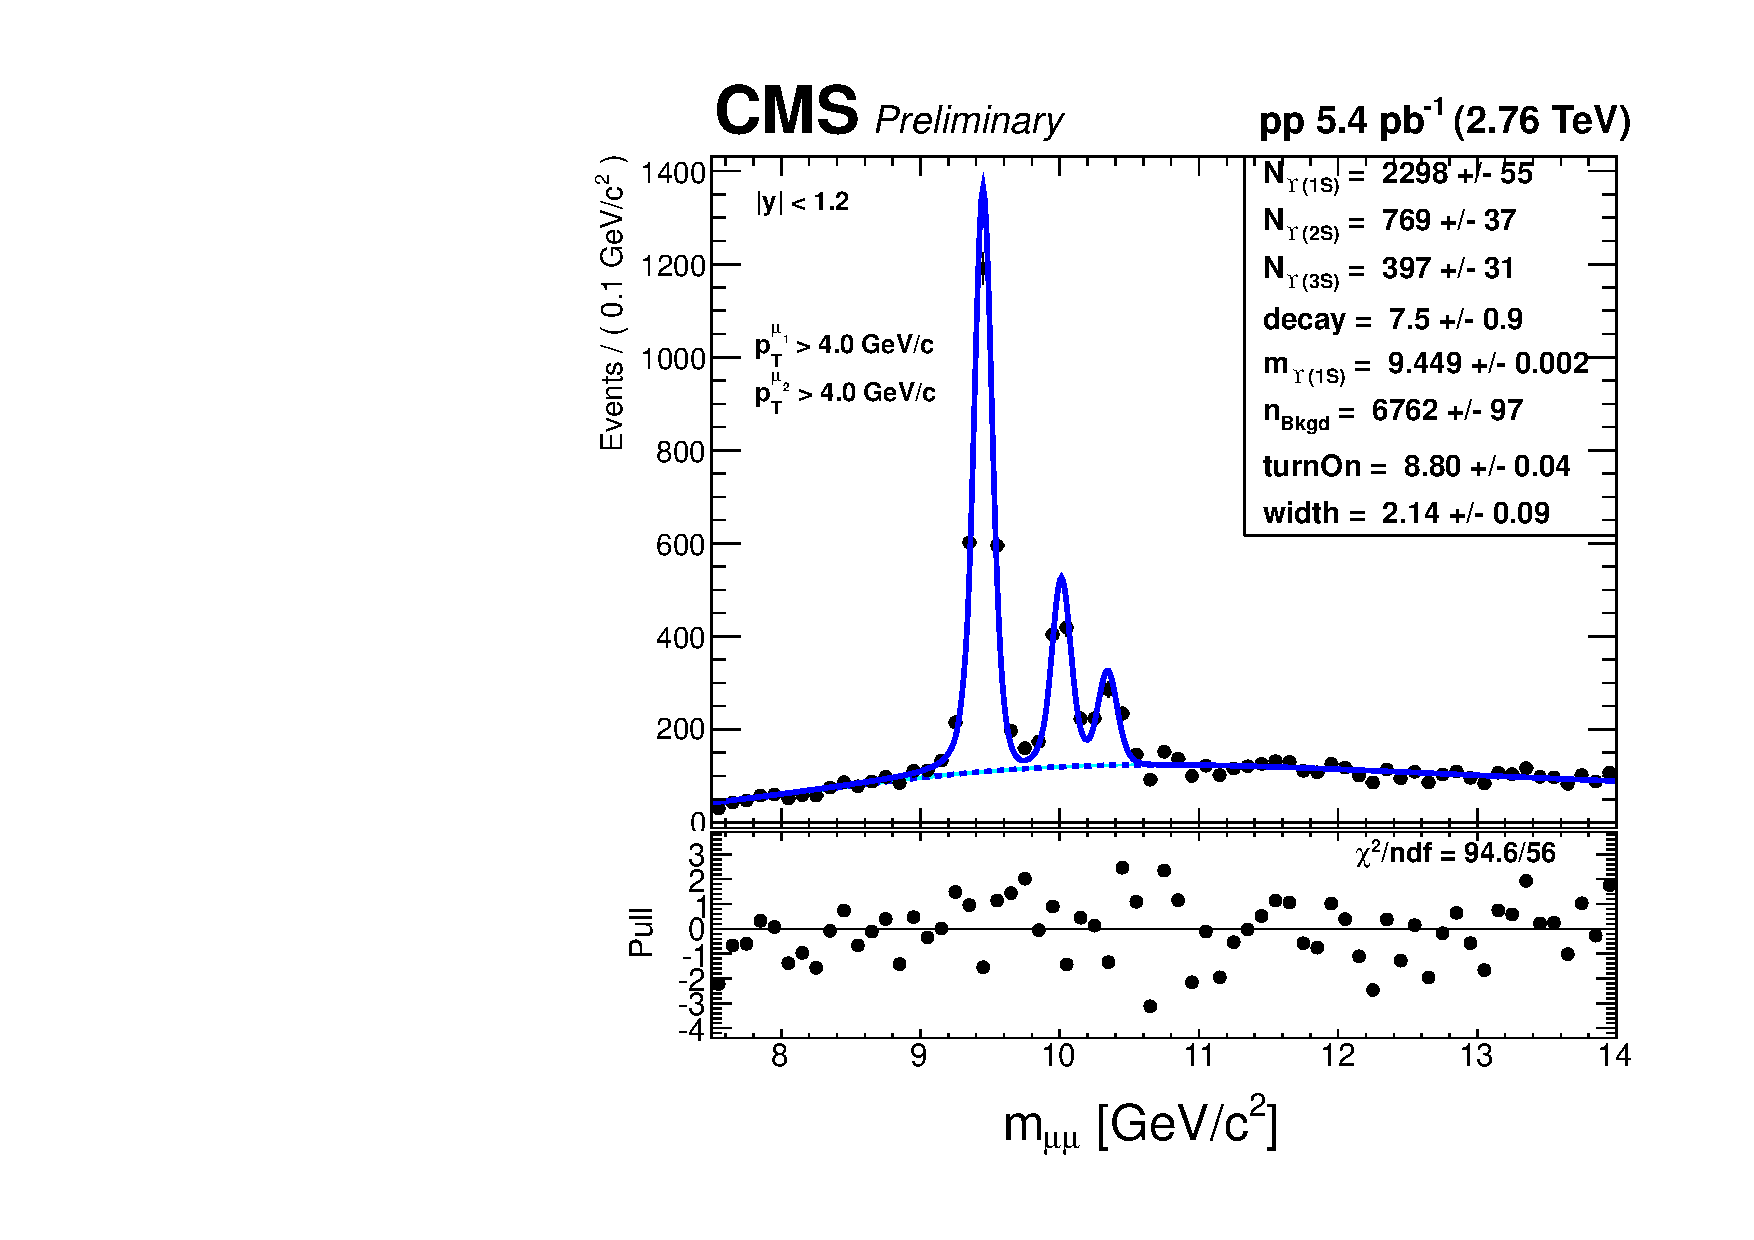
\includegraphics[width=0.49\textwidth]{Chapters/aYield/pp/pt_4_4/Rap/Rap_0_1p2/pp2p76tev_Rap_0_1p2_fsr1.pdf}
  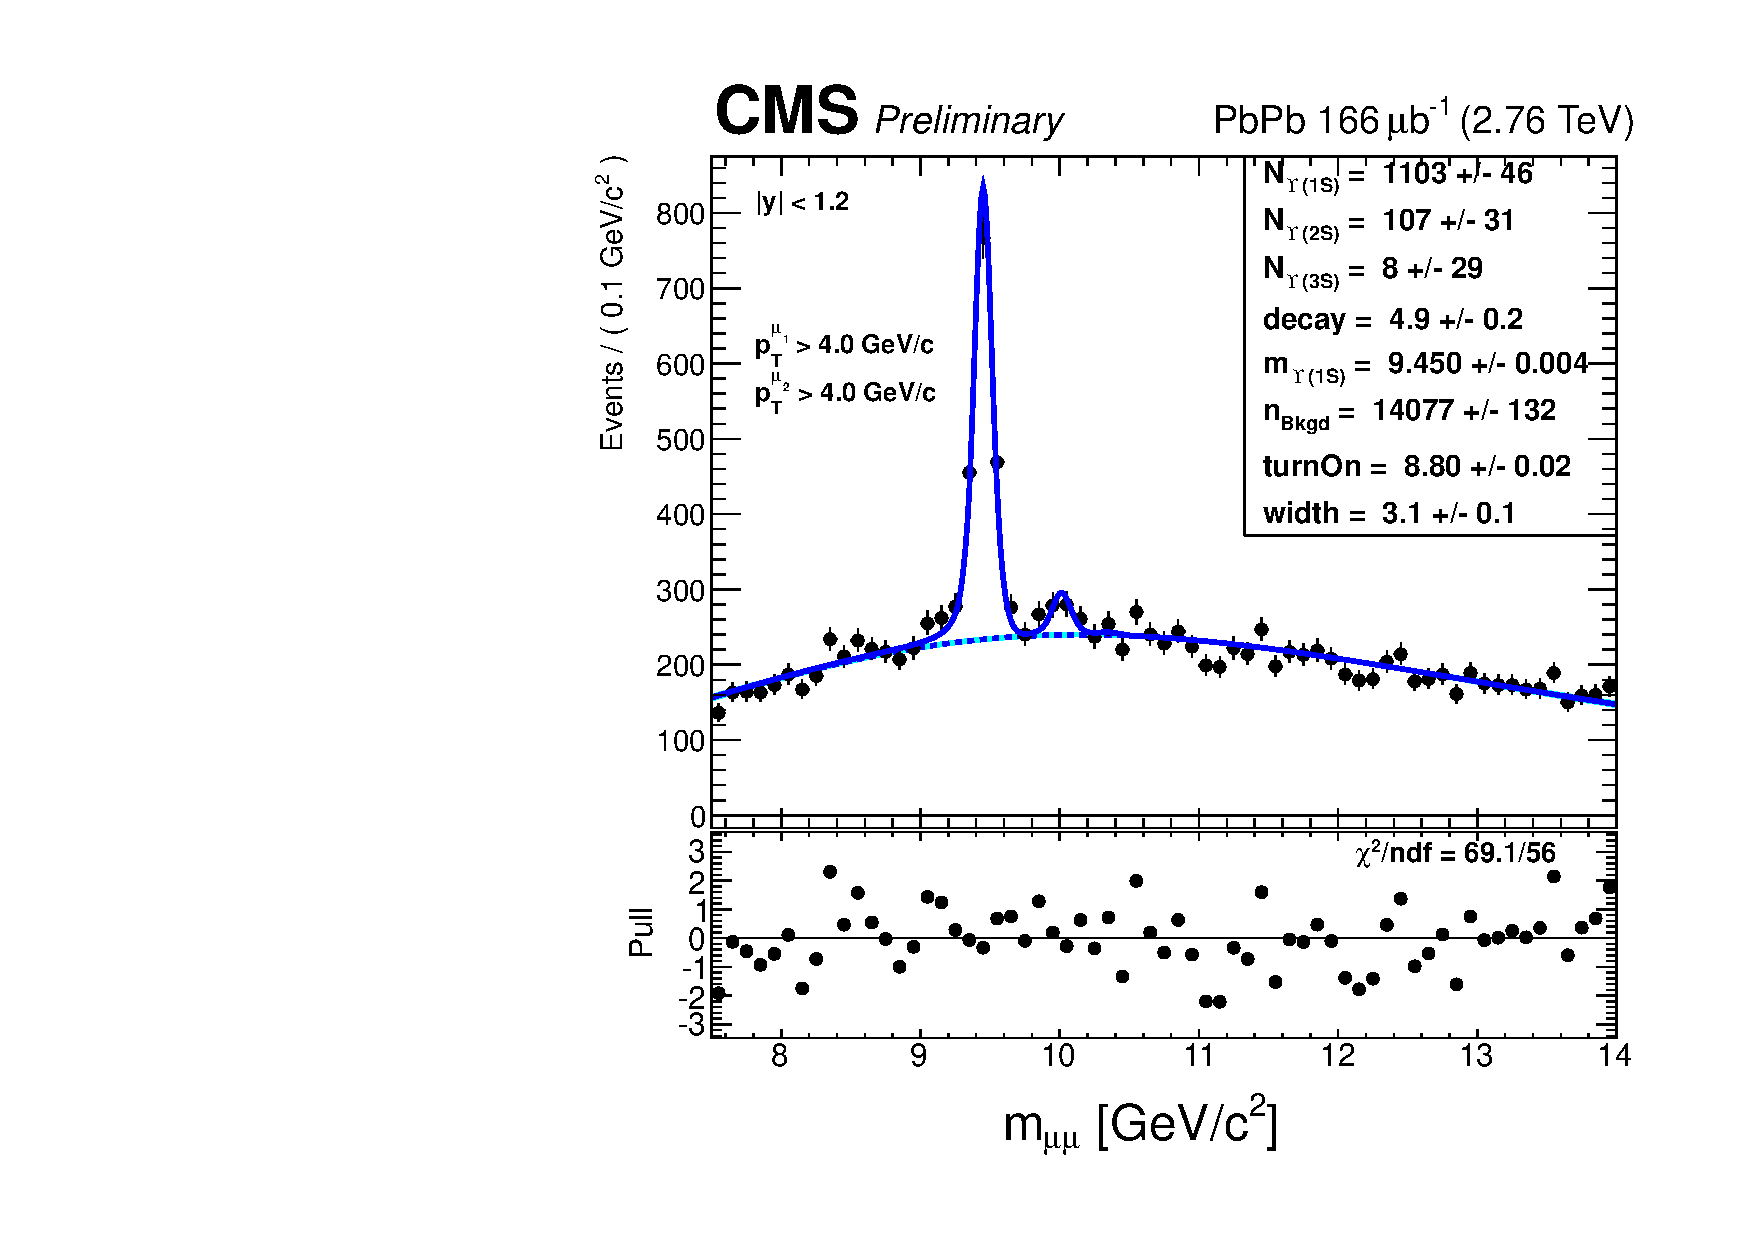
\includegraphics[width=0.49\textwidth]{Chapters/aYield/PbPb/pt_4_4/Rap/Rap_0_1p2/PbPb_Rap_0_1p2_fsr1.pdf}
  \caption{Fits to pp (left) and PbPb (right) datasets with tight muon cuts ($\PgUb$ analysis) in the bin $y\in [0 - 1.2]$.}
  \label{fig:YieldsErfExp_y2Sa} 
\end{figure}
\begin{figure}   
    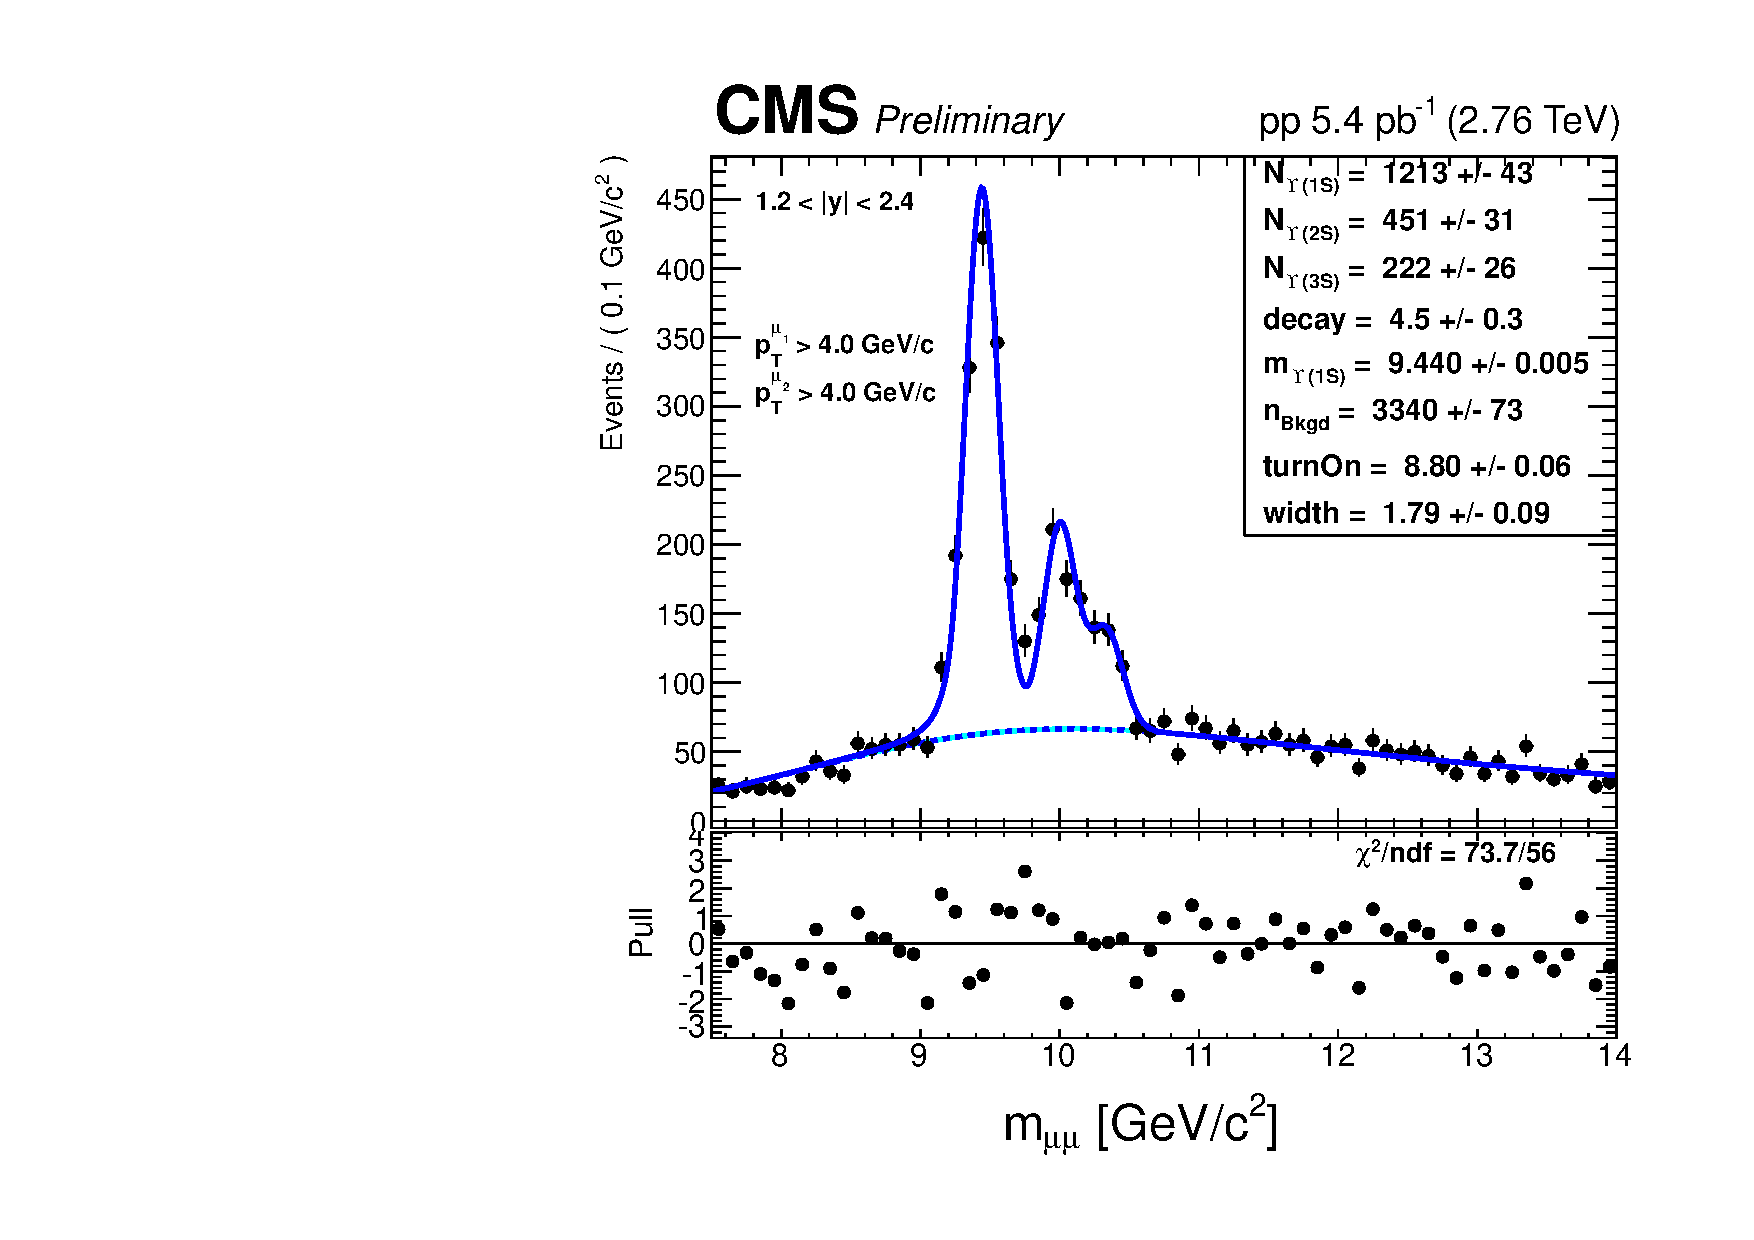
\includegraphics[width=0.49\textwidth]{Chapters/aYield/pp/pt_4_4/Rap/Rap_1p2_2p4/pp2p76tev_Rap_1p2_2p4_fsr1.pdf}
  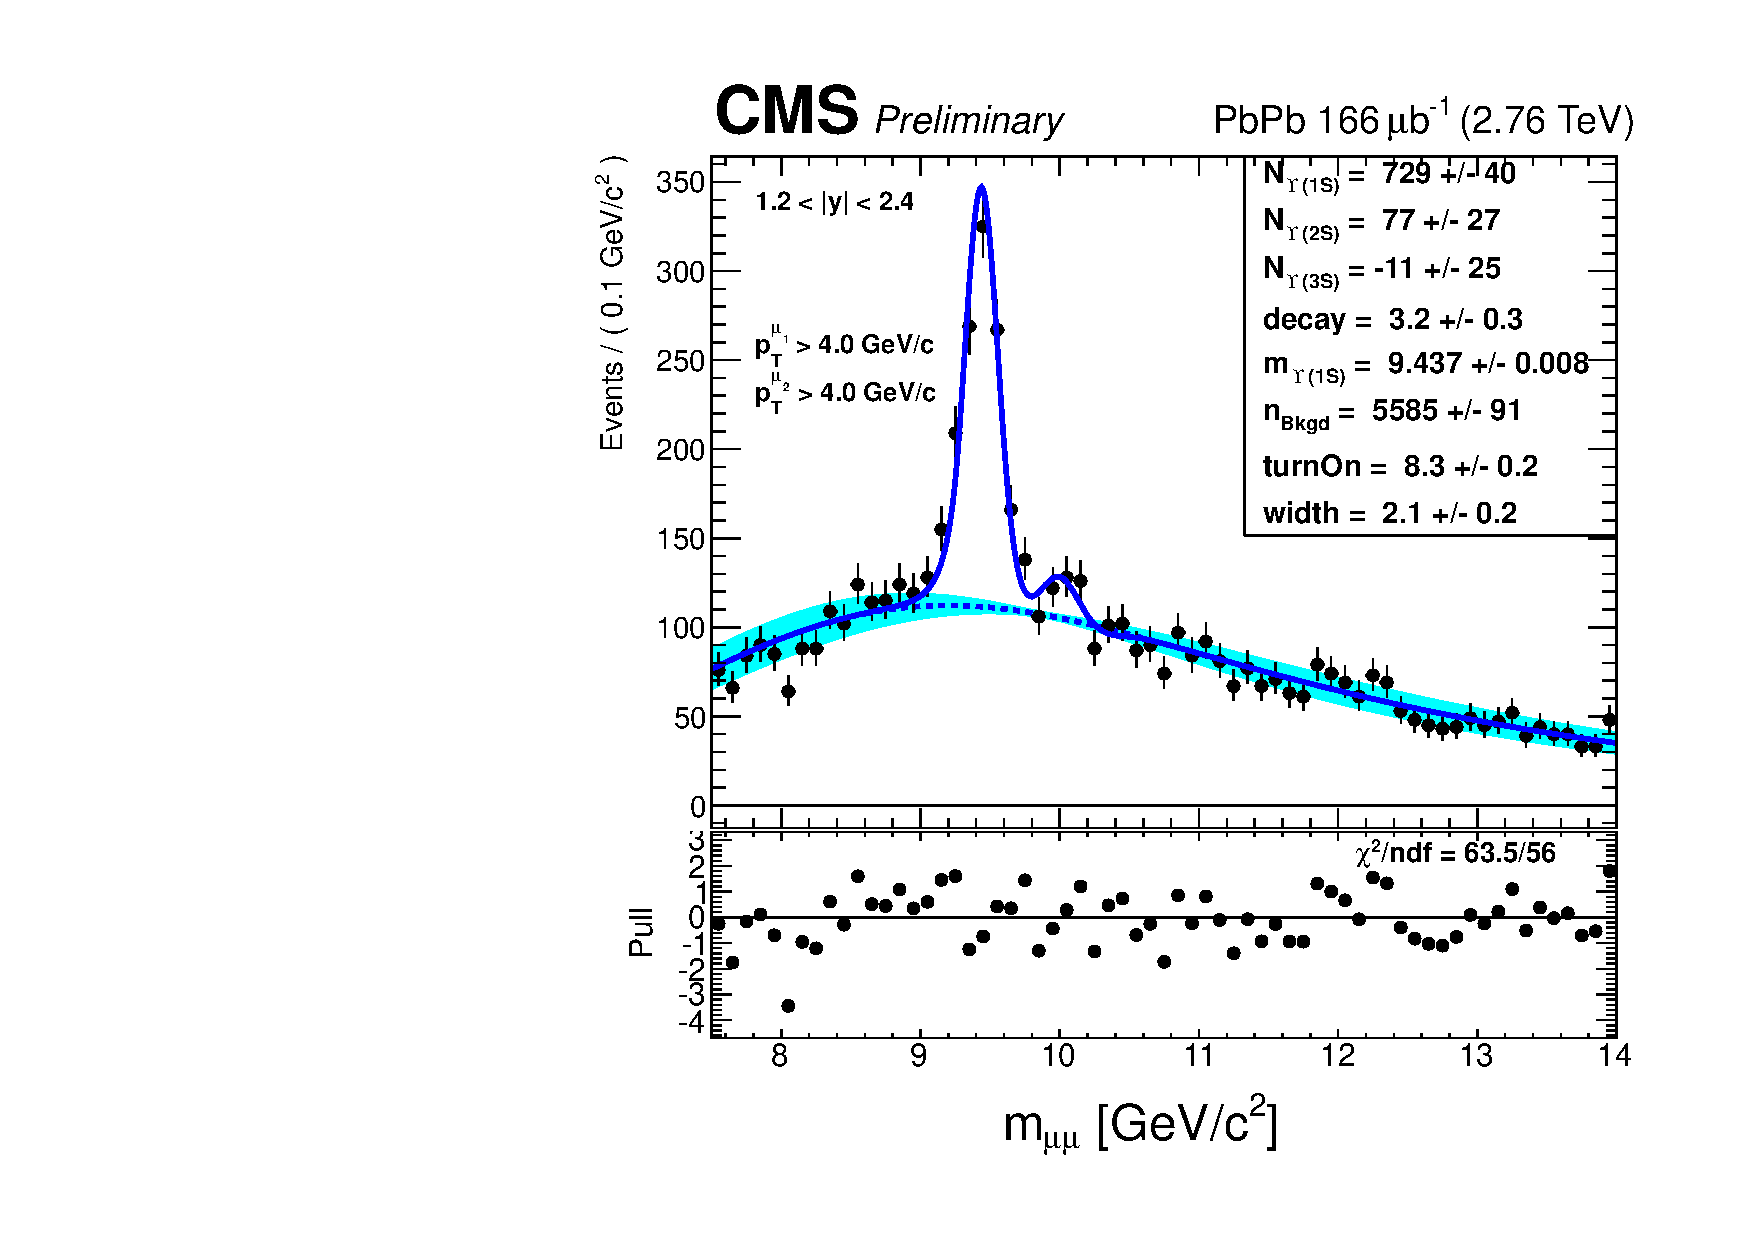
\includegraphics[width=0.49\textwidth]{Chapters/aYield/PbPb/pt_4_4/Rap/Rap_1p2_2p4/PbPb_Rap_1p2_2p4_fsr1.pdf}
  \caption{Same as Figure~\ref{fig:YieldsErfExp_y2Sa} in the bin $y\in [1.2 - 2.4]$.}
  \label{fig:YieldsErfExp_y2Sb} 
\end{figure}
\clearpage
\subsection{$pp$ cross section measurements for excited states}

Figures from~\ref{fig:YieldsErfExp_2S3Sa} to~\ref{fig:YieldsErfExp_pt2S3Sf}
present the \pt\ and rapidity bins of the \PgUb\ and \PgUc\ cross
section in $pp$ collisions.

\begin{figure}
  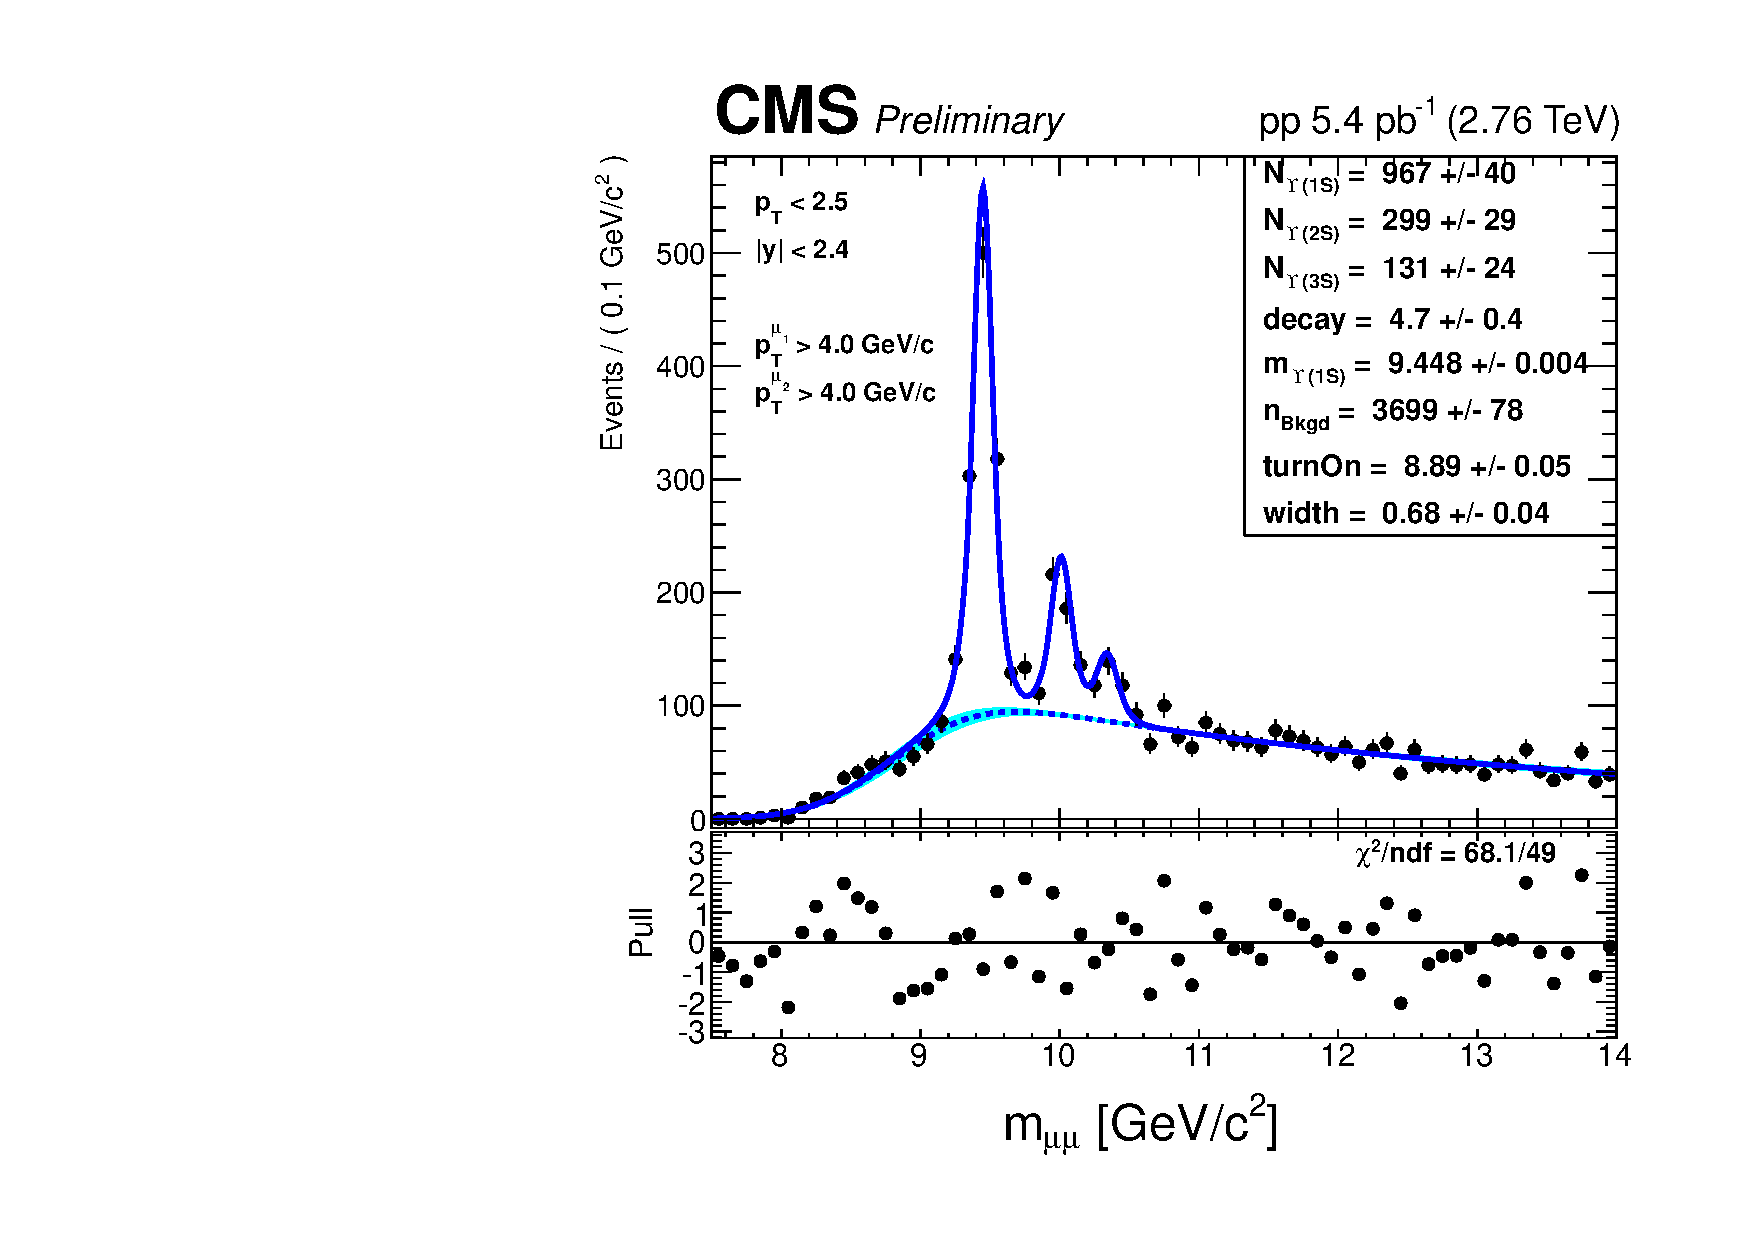
\includegraphics[width=0.49\textwidth]{Chapters/aYield/pp/pt_4_4/Pt/Pt_0_2p5/pp2p76tev_Pt_0_2p5_fsr1.pdf}  
  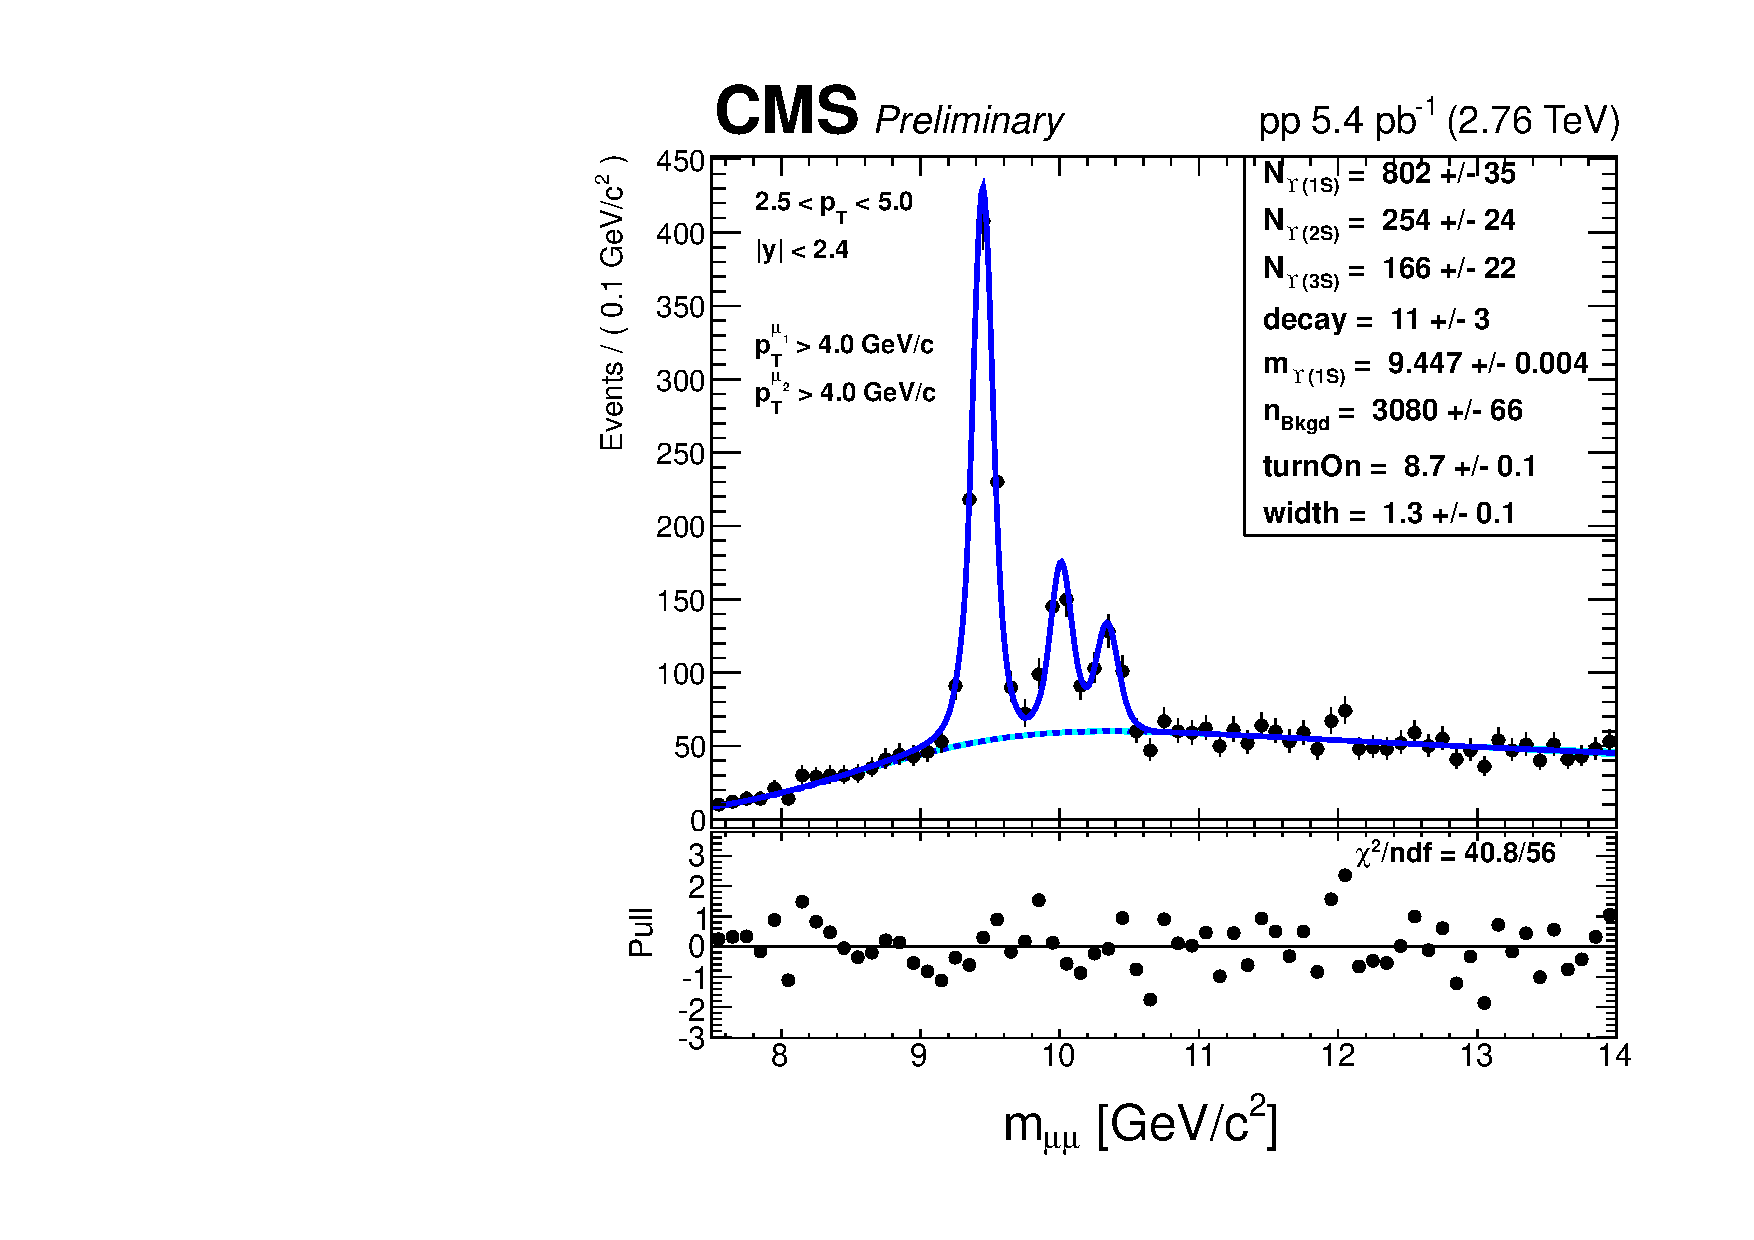
\includegraphics[width=0.49\textwidth]{Chapters/aYield/pp/pt_4_4/Pt/Pt_2p5_5/pp2p76tev_Pt_2p5_5_fsr1.pdf}  
  \caption{Fits to the $pp$ dataset with the tight muon \pt\ cut
    applied, for the extraction of the $pp$ \PgUb\ and \PgUc\ cross
    sections in fine bins of \pt. Left:$\pt~[{\rm GeV}/c]\in [0 - 2.5]$. Right:$\pt~[{\rm GeV}/c]\in [2.5 - 5]$.}
  \label{fig:YieldsErfExp_2S3Sa} 
\end{figure}
\begin{figure}
  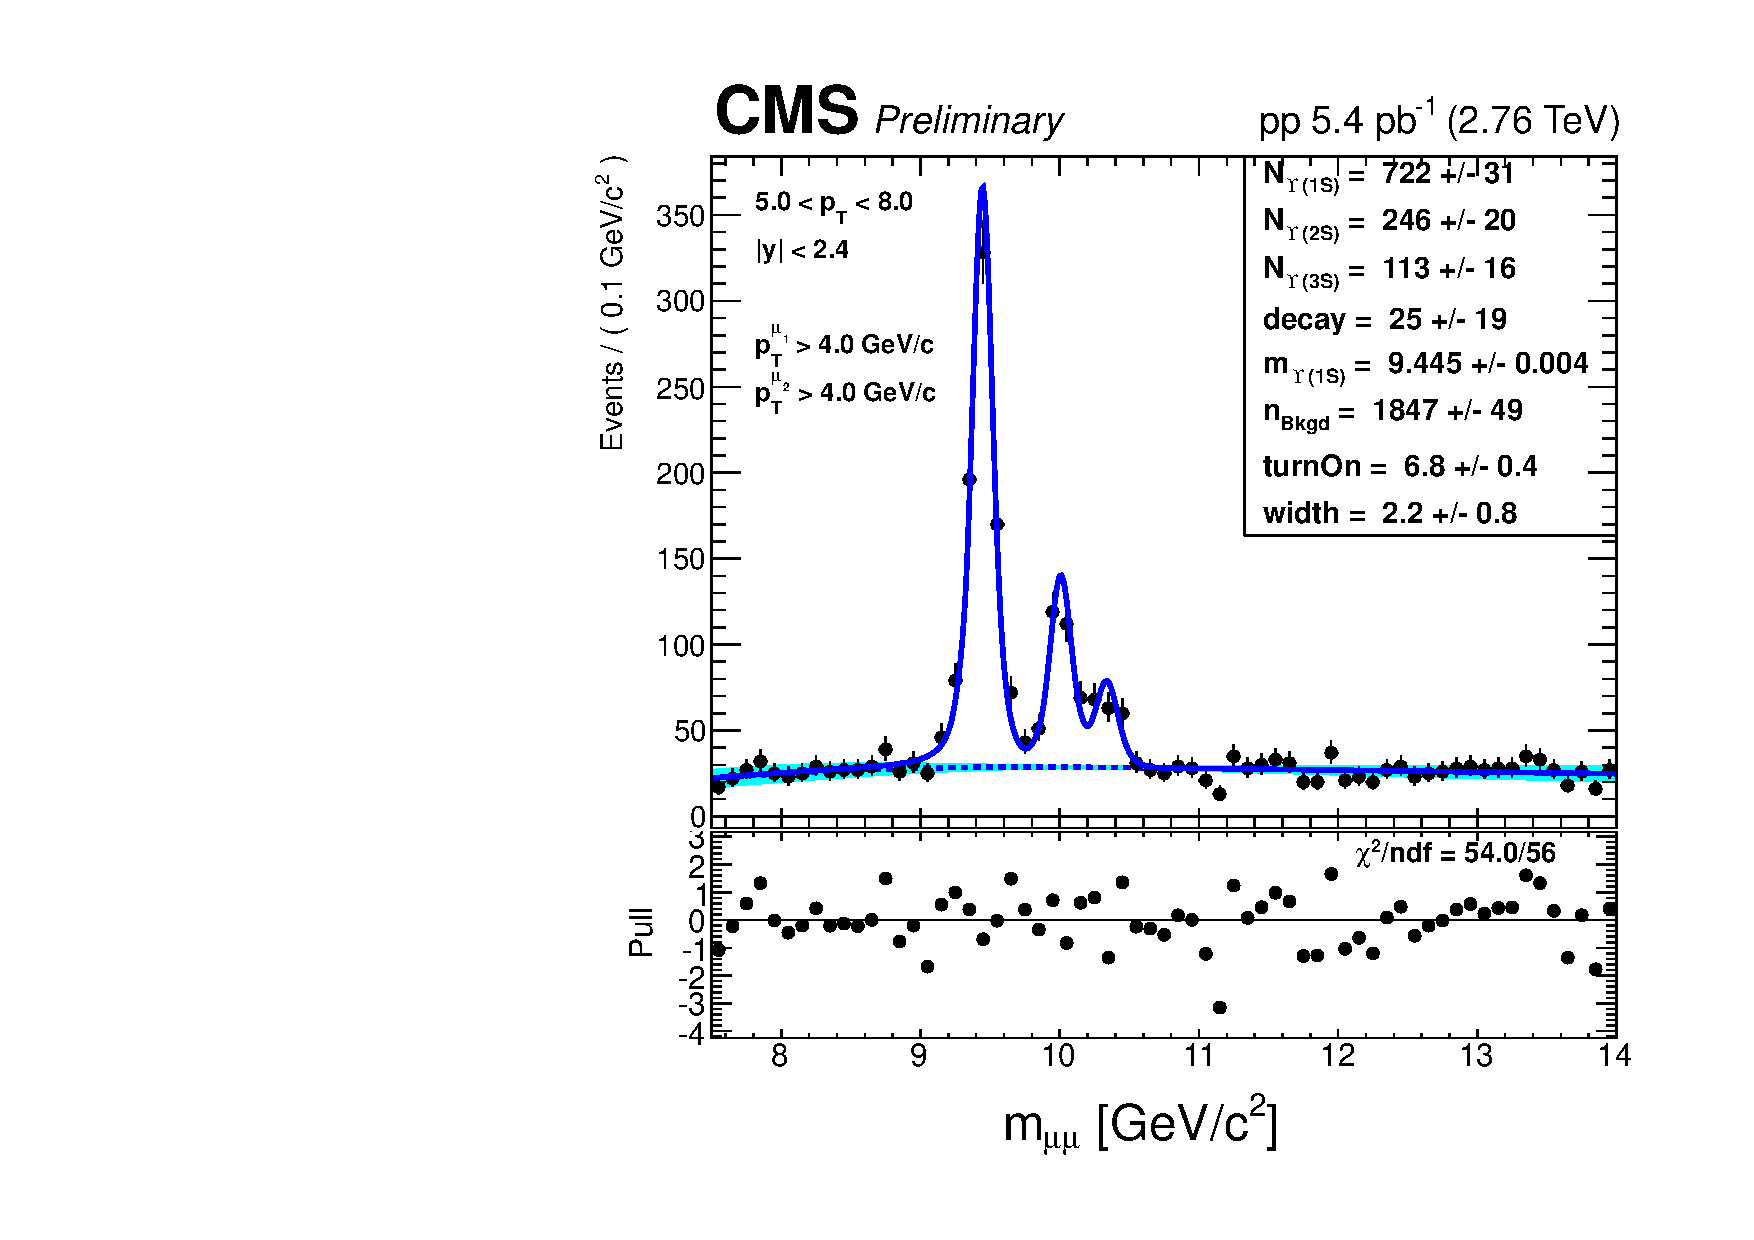
\includegraphics[width=0.49\textwidth]{Chapters/aYield/pp/pt_4_4/Pt/Pt_5_8/pp2p76tev_Pt_5_8_fsr1.pdf}  
  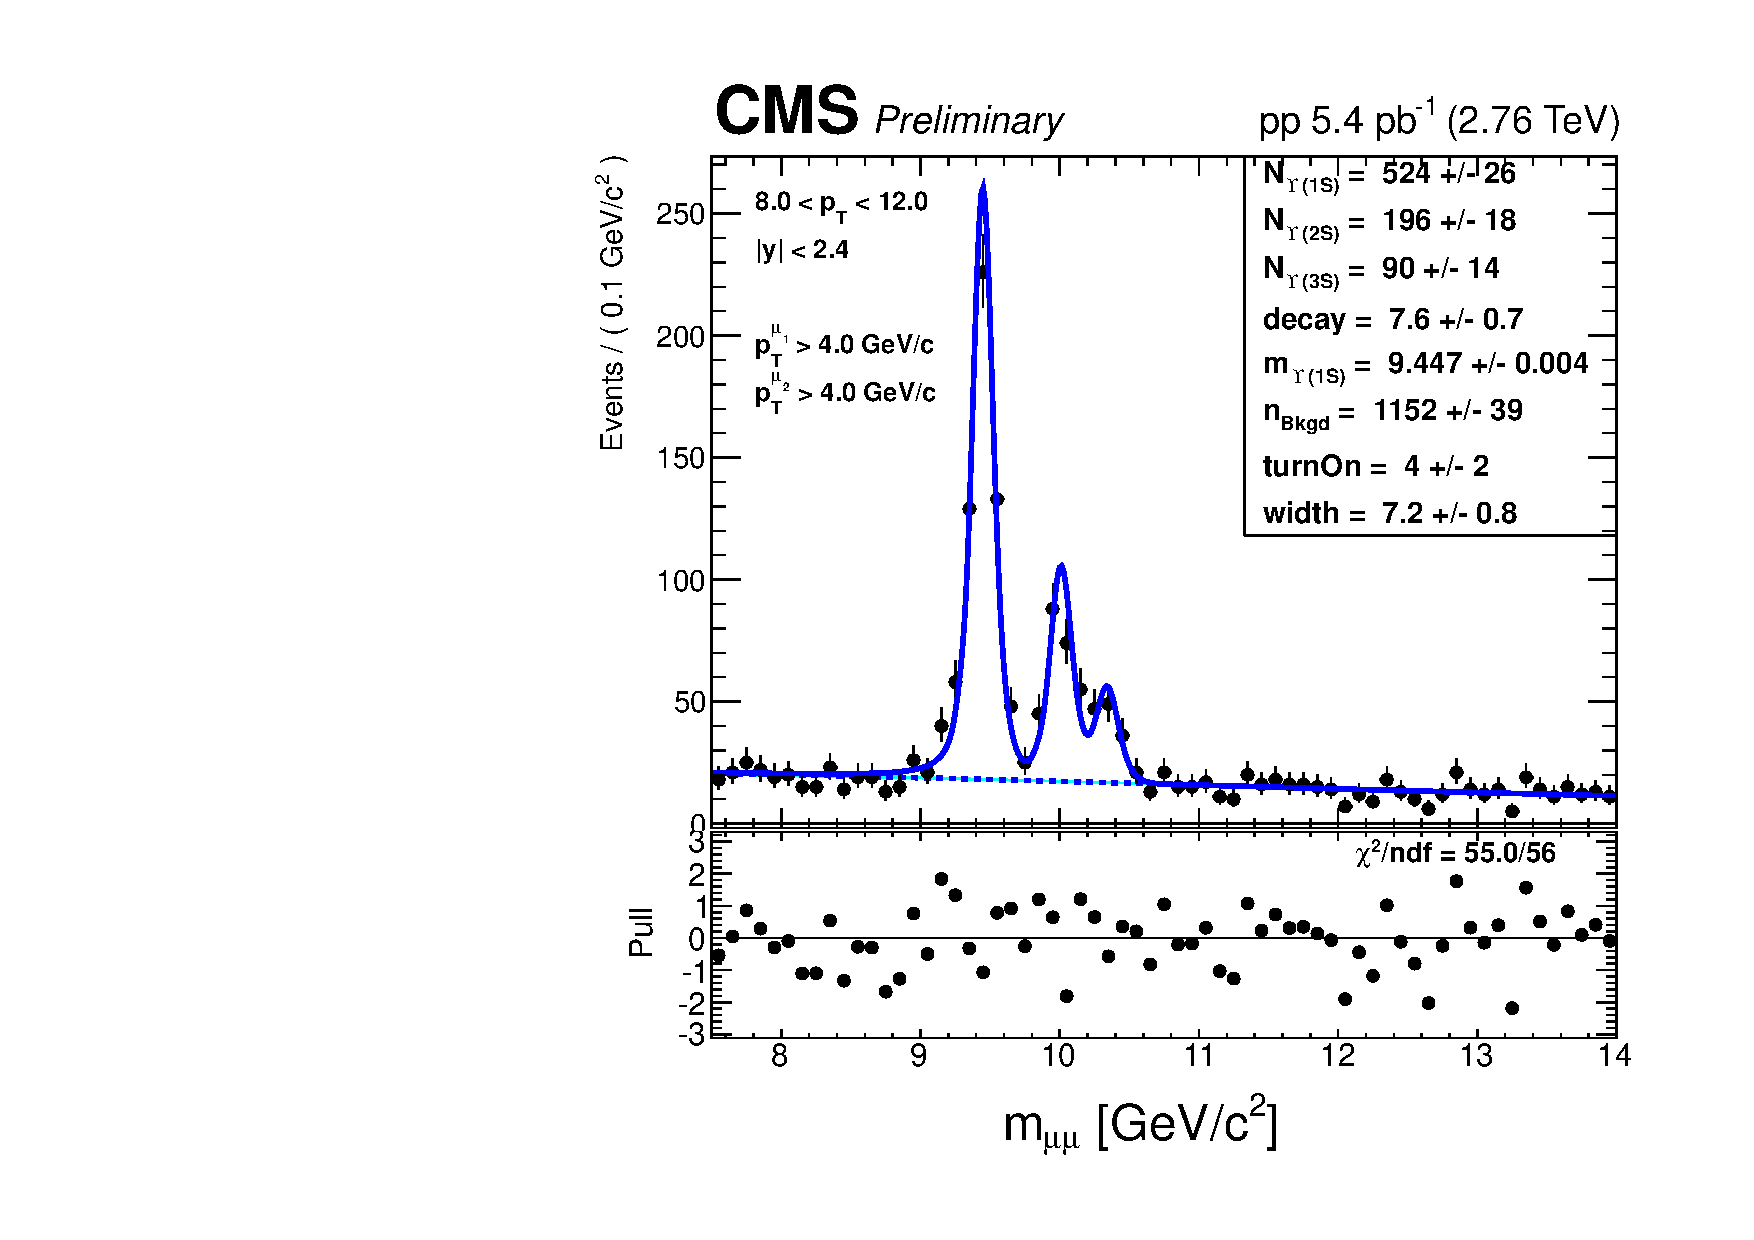
\includegraphics[width=0.49\textwidth]{Chapters/aYield/pp/pt_4_4/Pt/Pt_8_12/pp2p76tev_Pt_8_12_fsr1.pdf}  
  \caption{Fits to the $pp$ dataset with the tight muon \pt\ cut
    applied, for the extraction of the $pp$ \PgUb\ and \PgUc\ cross
    sections in fine bins of \pt. Left:$\pt~[{\rm GeV}/c]\in [5 - 8]$. Right:$\pt~[{\rm GeV}/c]\in [8 - 12]$.}
  \label{fig:YieldsErfExp_2S3Sb} 
\end{figure}
\begin{figure}
  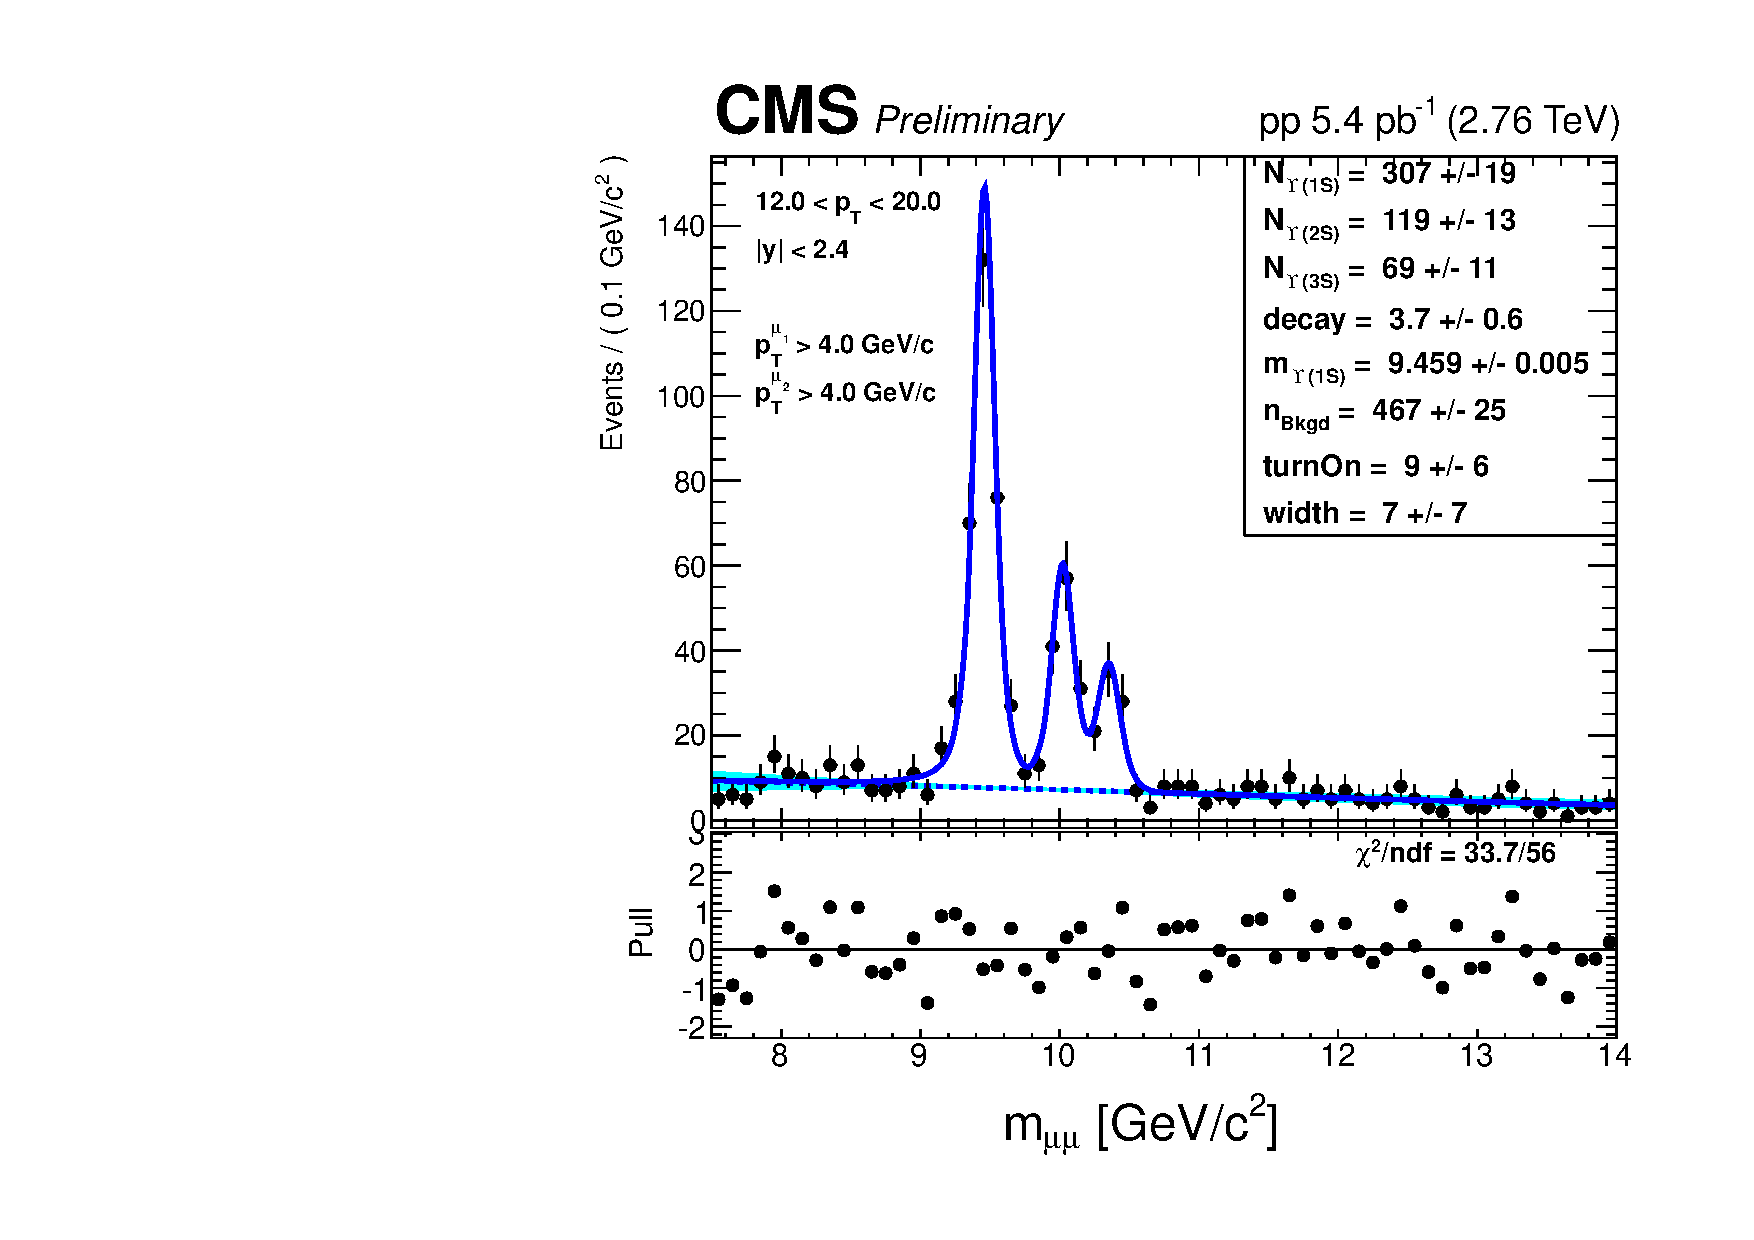
\includegraphics[width=0.49\textwidth]{Chapters/aYield/pp/pt_4_4/Pt/Pt_12_20/pp2p76tev_Pt_12_20_fsr1.pdf}  
  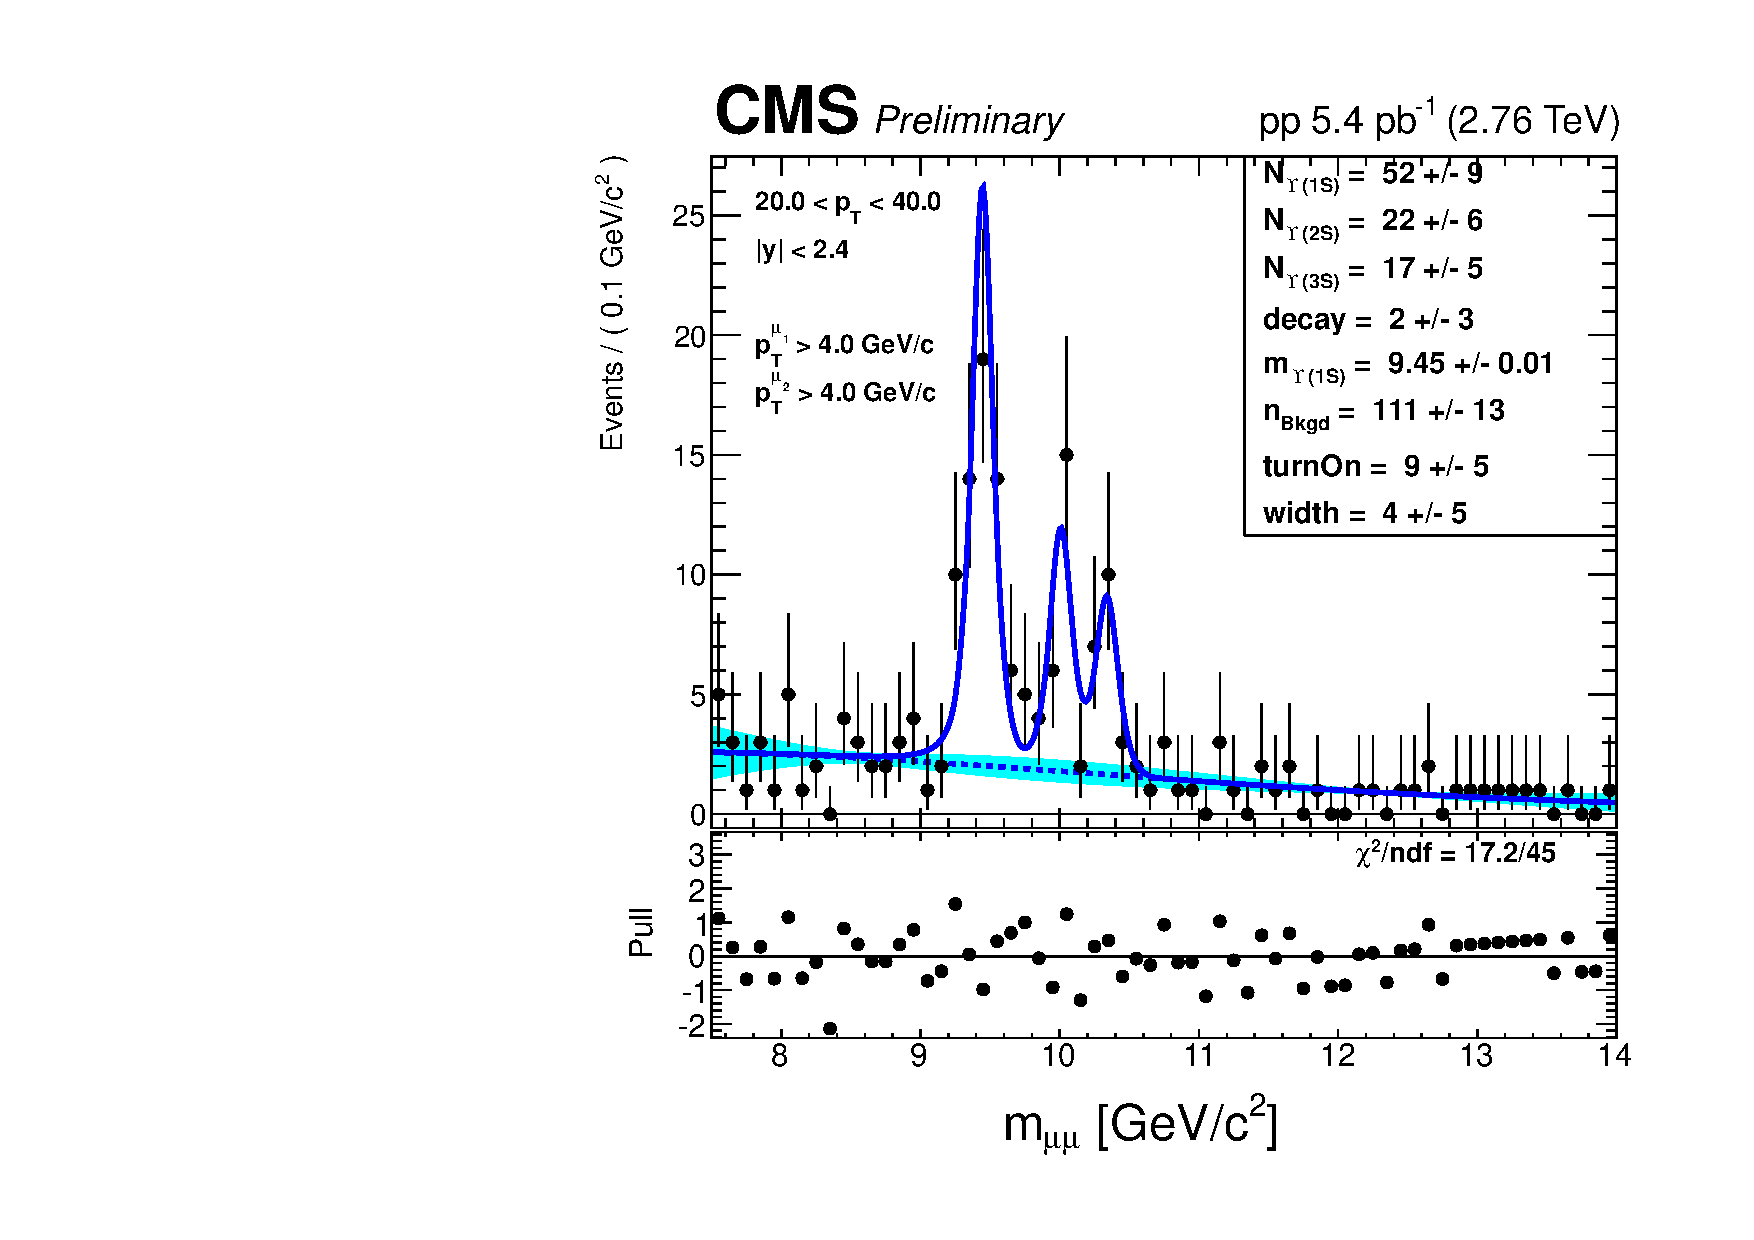
\includegraphics[width=0.49\textwidth]{Chapters/aYield/pp/pt_4_4/Pt/Pt_20_40/pp2p76tev_Pt_20_40_fsr1.pdf}  
  \caption{Fits to the $pp$ dataset with the tight muon \pt\ cut
    applied, for the extraction of the $pp$ \PgUb\ and \PgUc\ cross
    sections in fine bins of \pt. Left:$\pt~[{\rm GeV}/c]\in [12 - 20]$. Right:$\pt~[{\rm GeV}/c]\in [20 - 40]$.}
  \label{fig:YieldsErfExp_2S3Sc} 
\end{figure}
\begin{figure}
  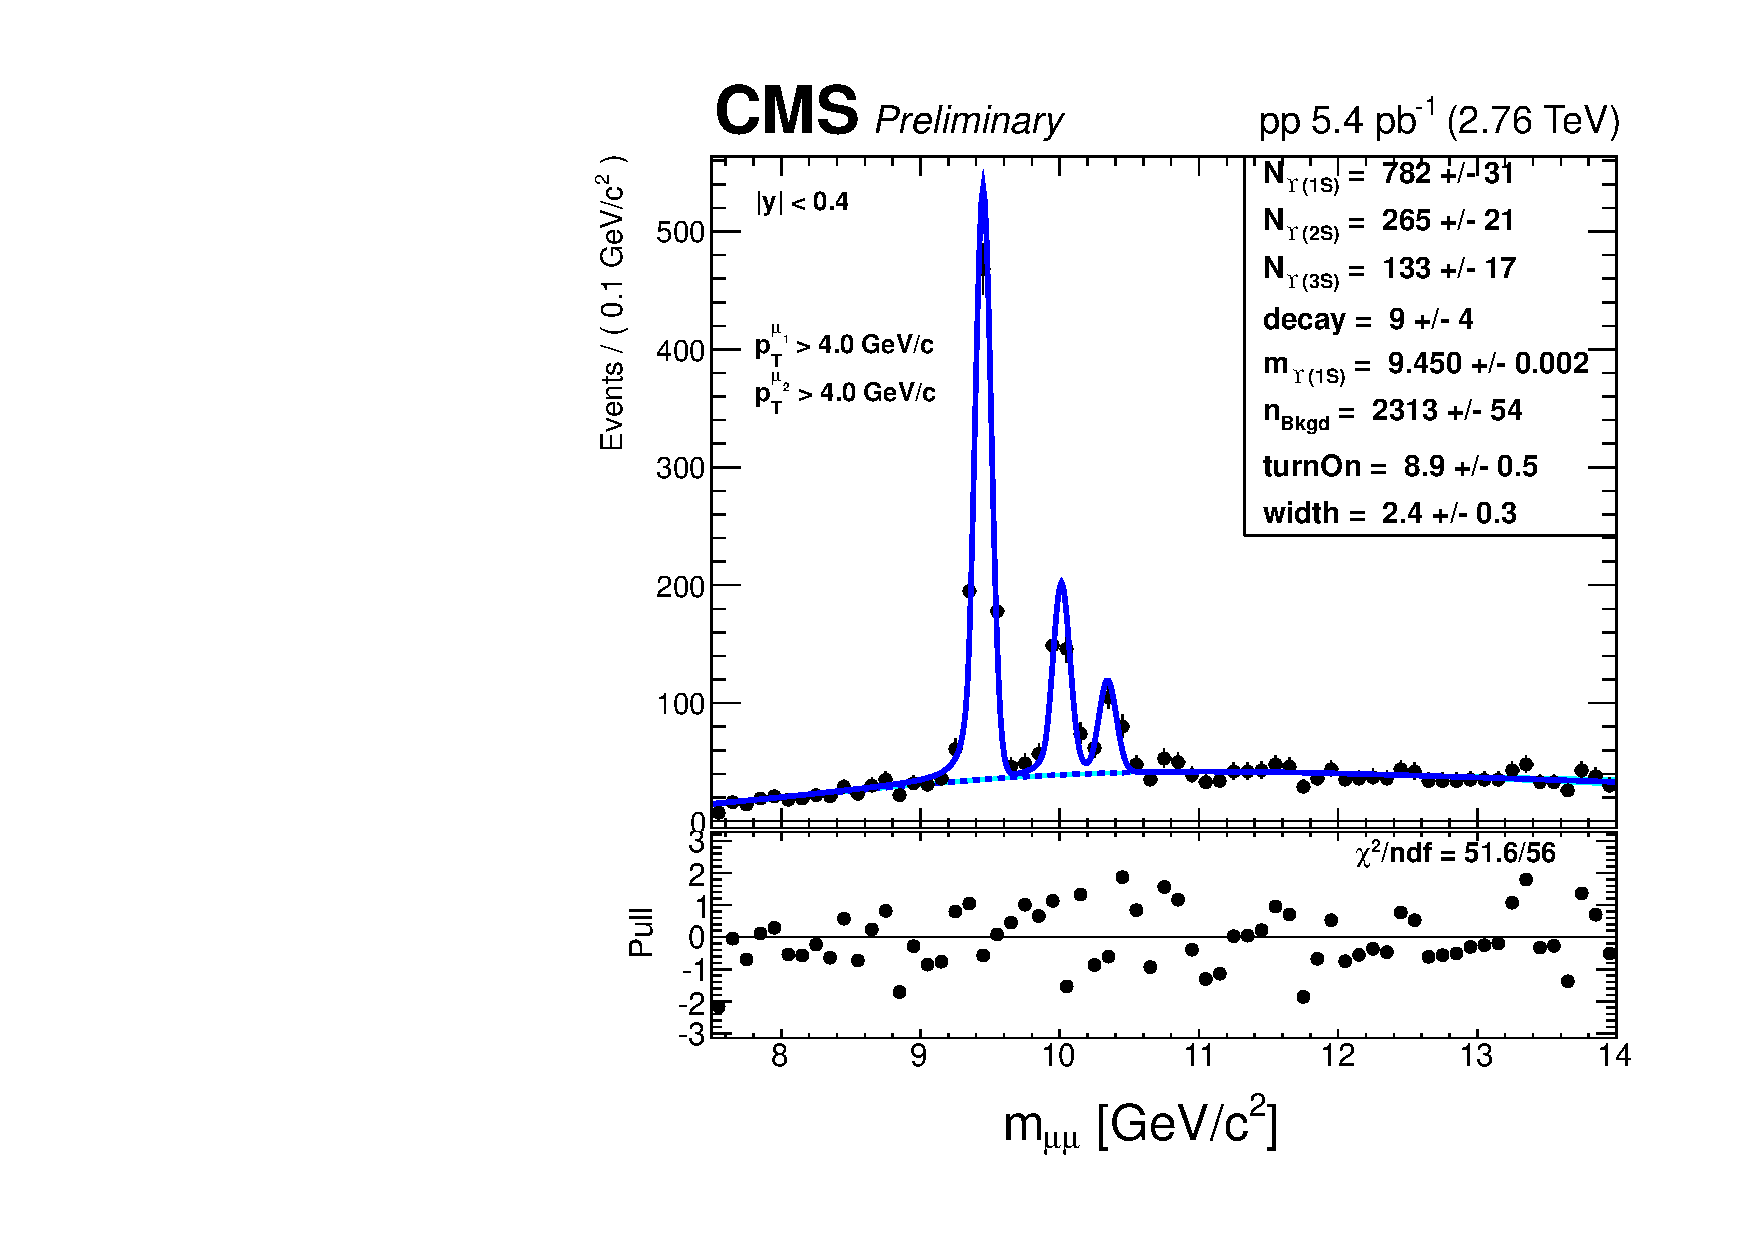
\includegraphics[width=0.49\textwidth]{Chapters/aYield/pp/pt_4_4/Rap/Rap_0_0p4/pp2p76tev_Rap_0_0p4_fsr1.pdf}  
  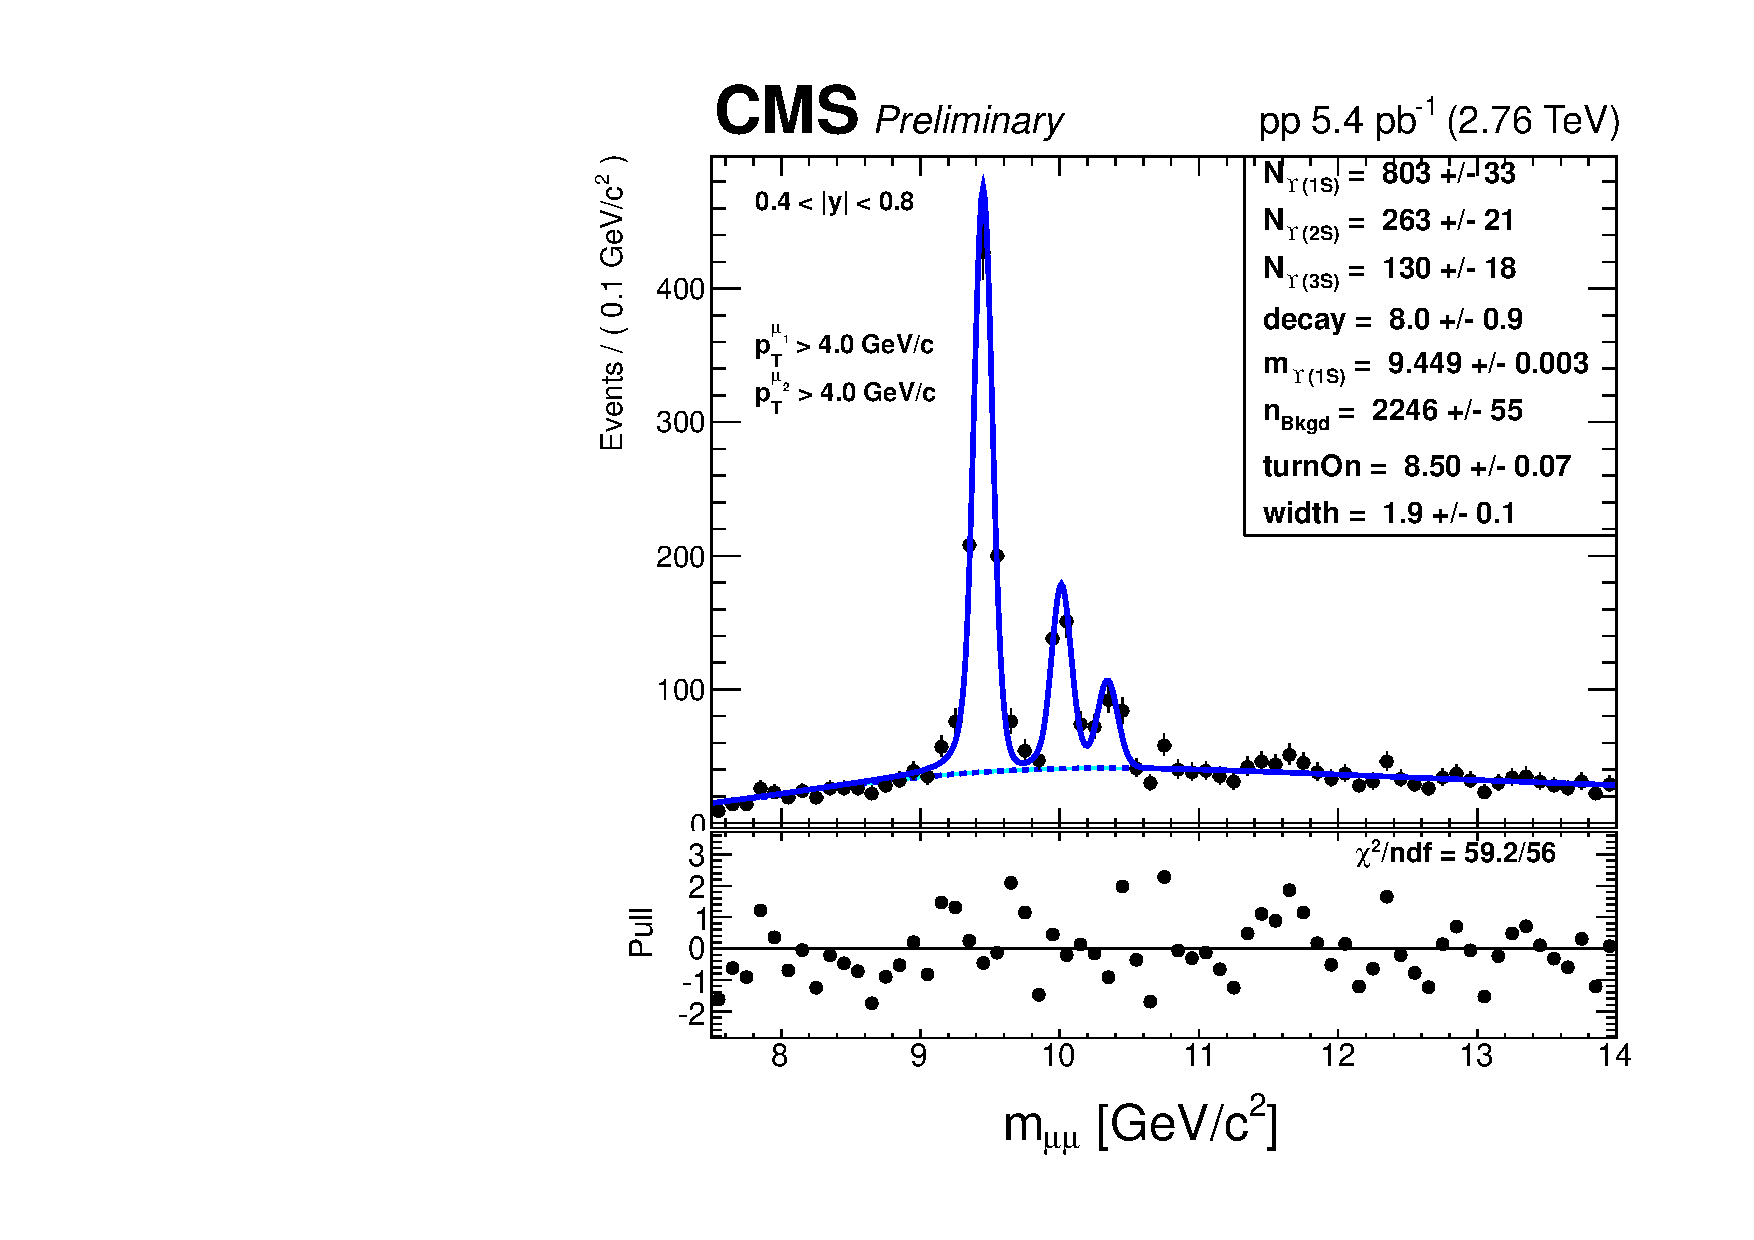
\includegraphics[width=0.49\textwidth]{Chapters/aYield/pp/pt_4_4/Rap/Rap_0p4_0p8/pp2p76tev_Rap_0p4_0p8_fsr1.pdf}  
  \caption{Fits to the $pp$ dataset with the tight muon \pt\ cut
    applied, for the extraction of the $pp$ \PgUb\ and \PgUc\ cross
    sections in fine bins of rapidity. Left:$y\in [0. - 0.4]$. Right:$y\in [0.4 - 0.8]$.}
  \label{fig:YieldsErfExp_2S3Sd} 
\end{figure}
\begin{figure}
  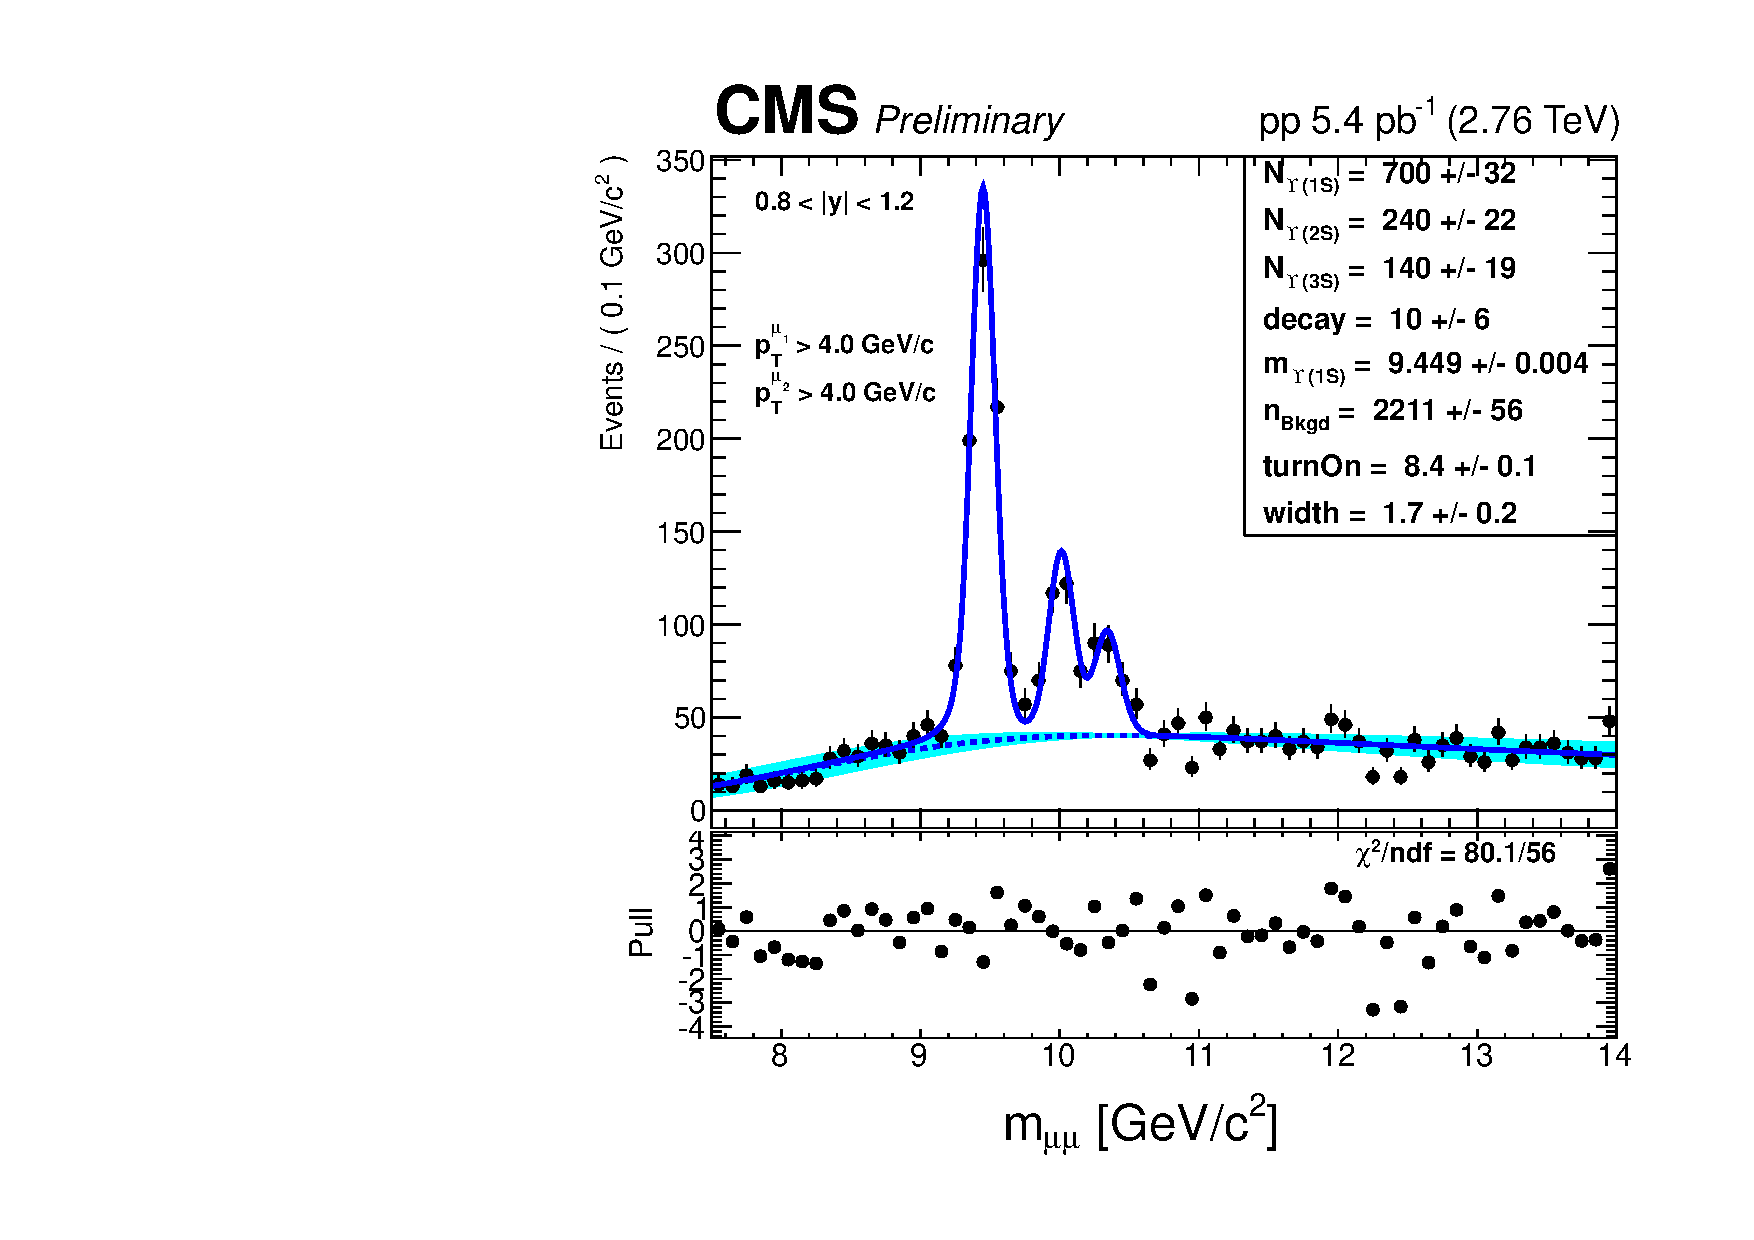
\includegraphics[width=0.49\textwidth]{Chapters/aYield/pp/pt_4_4/Rap/Rap_0p8_1p2/pp2p76tev_Rap_0p8_1p2_fsr1.pdf}  
  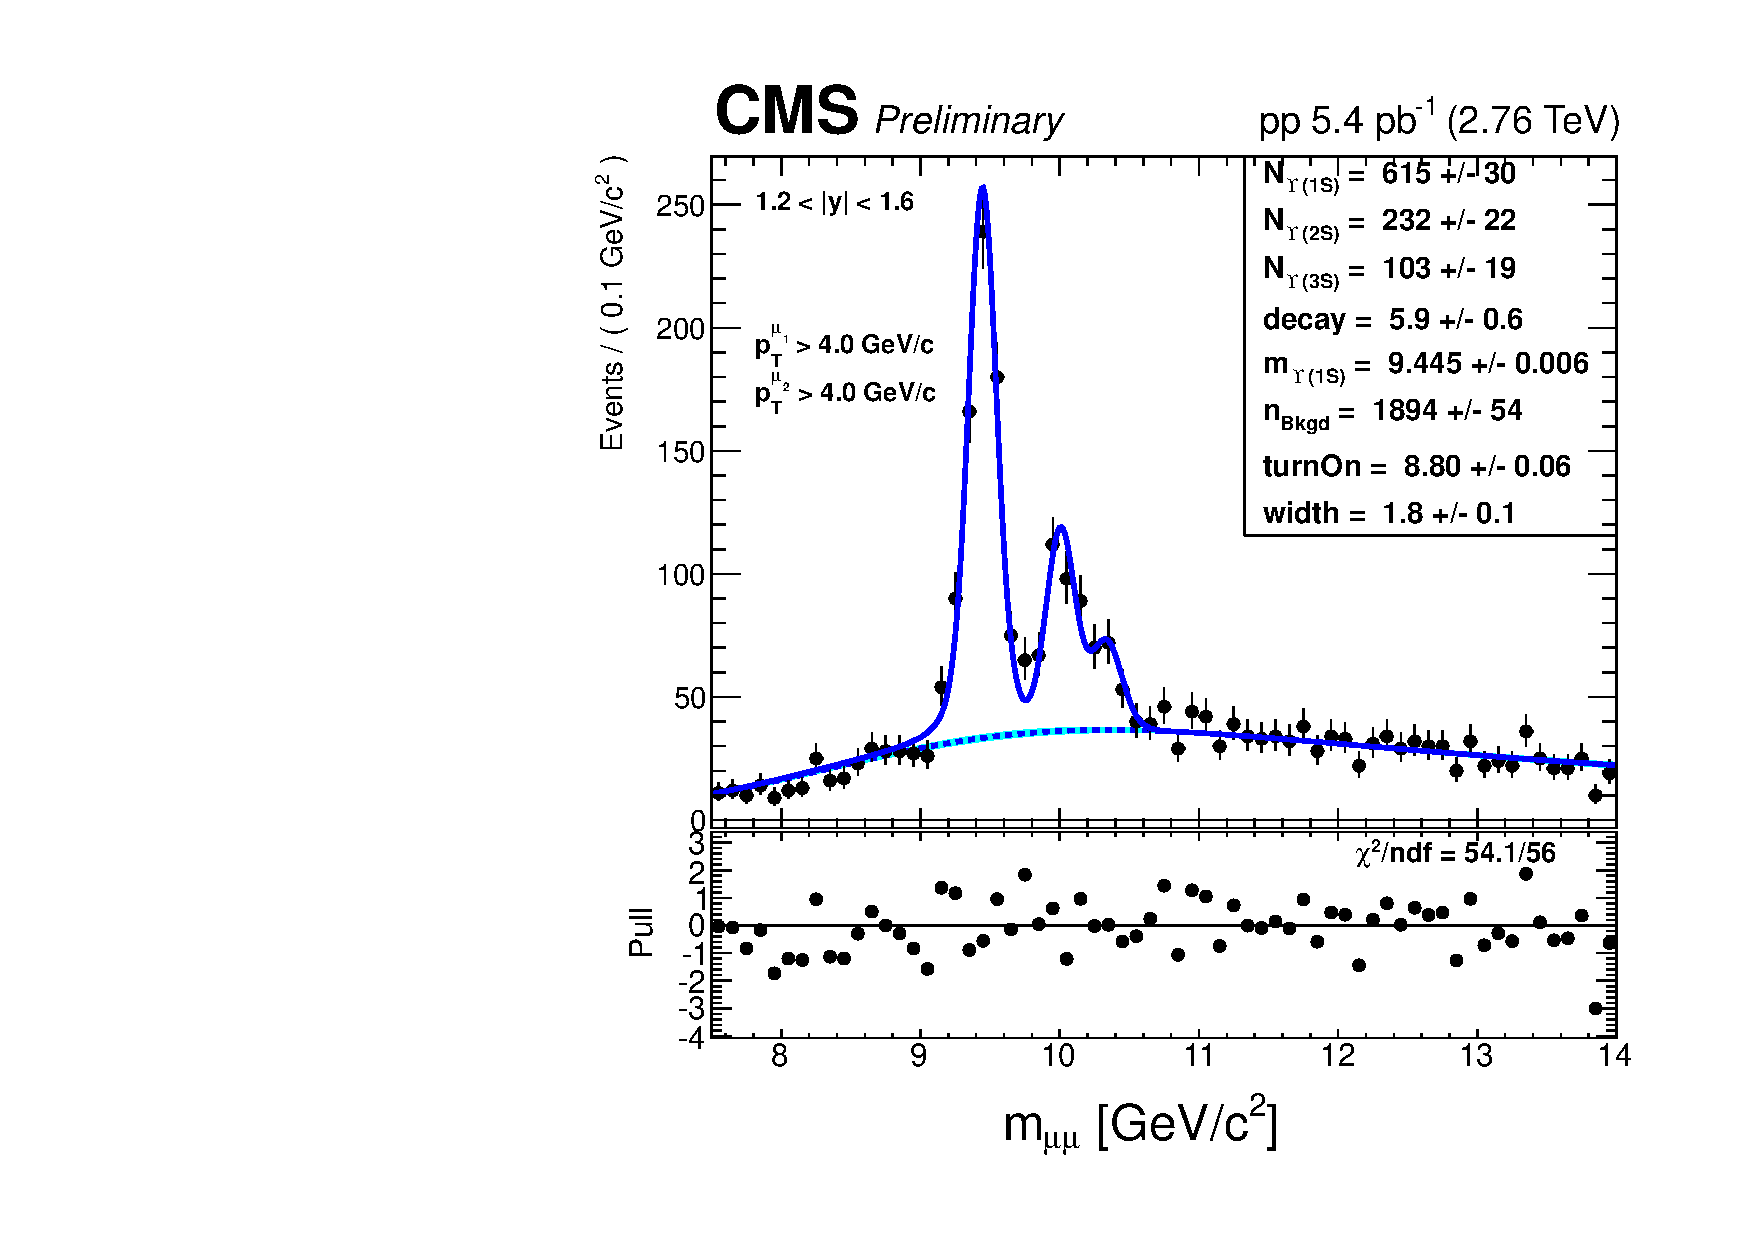
\includegraphics[width=0.49\textwidth]{Chapters/aYield/pp/pt_4_4/Rap/Rap_1p2_1p6/pp2p76tev_Rap_1p2_1p6_fsr1.pdf}  
  \caption{Fits to the $pp$ dataset with the tight muon \pt\ cut
    applied, for the extraction of the $pp$ \PgUb\ and \PgUc\ cross
    sections in fine bins of rapidity. Left:$y\in [0.8 - 1.2]$. Right:$y\in [1.2 - 1.6]$.}
  \label{fig:YieldsErfExp_2S3Se} 
\end{figure}
\begin{figure}
  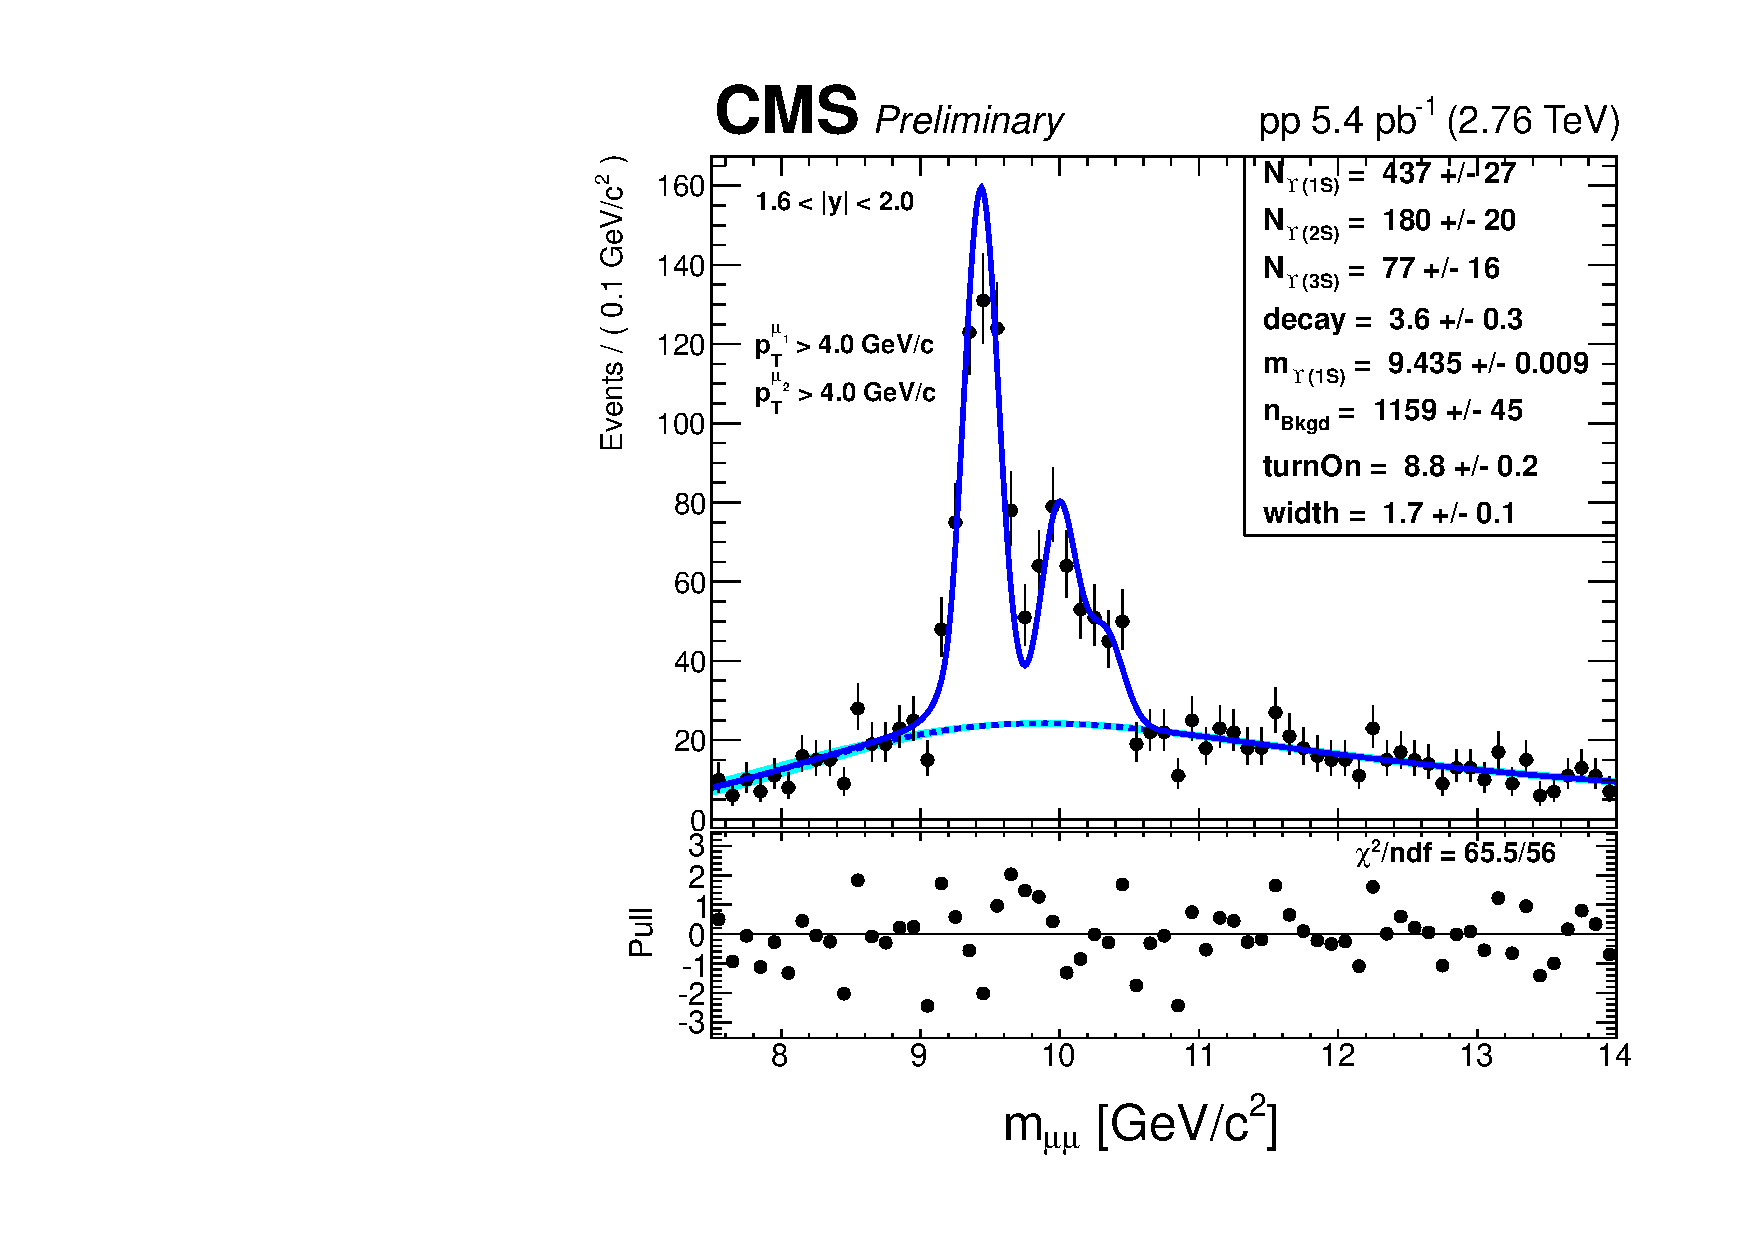
\includegraphics[width=0.49\textwidth]{Chapters/aYield/pp/pt_4_4/Rap/Rap_1p6_2/pp2p76tev_Rap_1p6_2_fsr1.pdf}  
  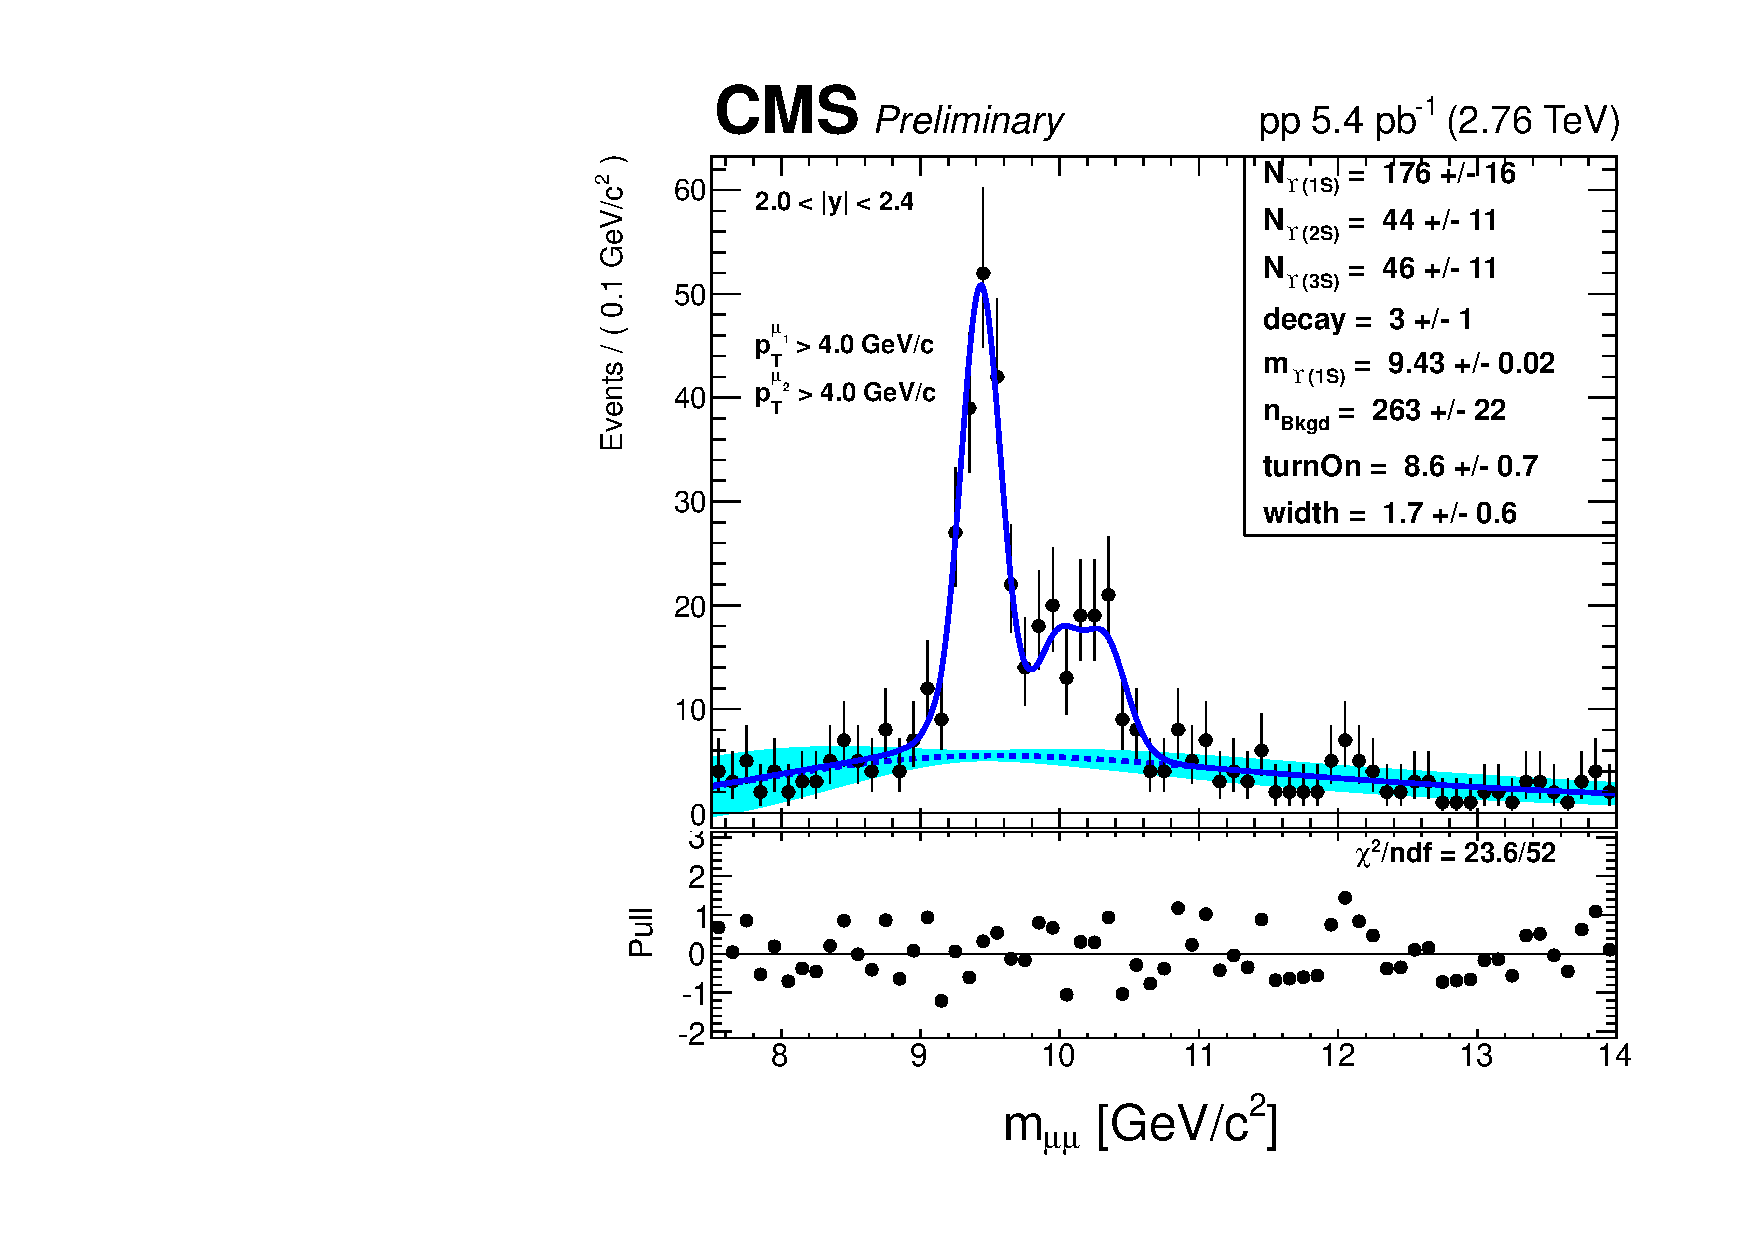
\includegraphics[width=0.49\textwidth]{Chapters/aYield/pp/pt_4_4/Rap/Rap_2_2p4/pp2p76tev_Rap_2_2p4_fsr1.pdf}  
  \caption{Fits to the $pp$ dataset with the tight muon \pt\ cut
    applied, for the extraction of the $pp$ \PgUb\ and \PgUc\ cross
    sections in fine bins of rapidity. Left:$y\in [1.6 - 2.0]$. Right:$y\in [2.0 - 2.4]$.}
  \label{fig:YieldsErfExp_2S3Sf} 
\end{figure}


\clearpage

\subsection{Centrality dependent analysis of PbPb yields}
\label{sec:figs_cent}
Figure~\ref{fig:YieldsCent1S},~\ref{fig:YieldsCent1SContd} report the centrality dependent fit results
for the \PgUa\ analysis,
and~\ref{fig:YieldsCent2S} report the centrality dependent fit
results of the \PgUb analysis.
\begin{figure}
 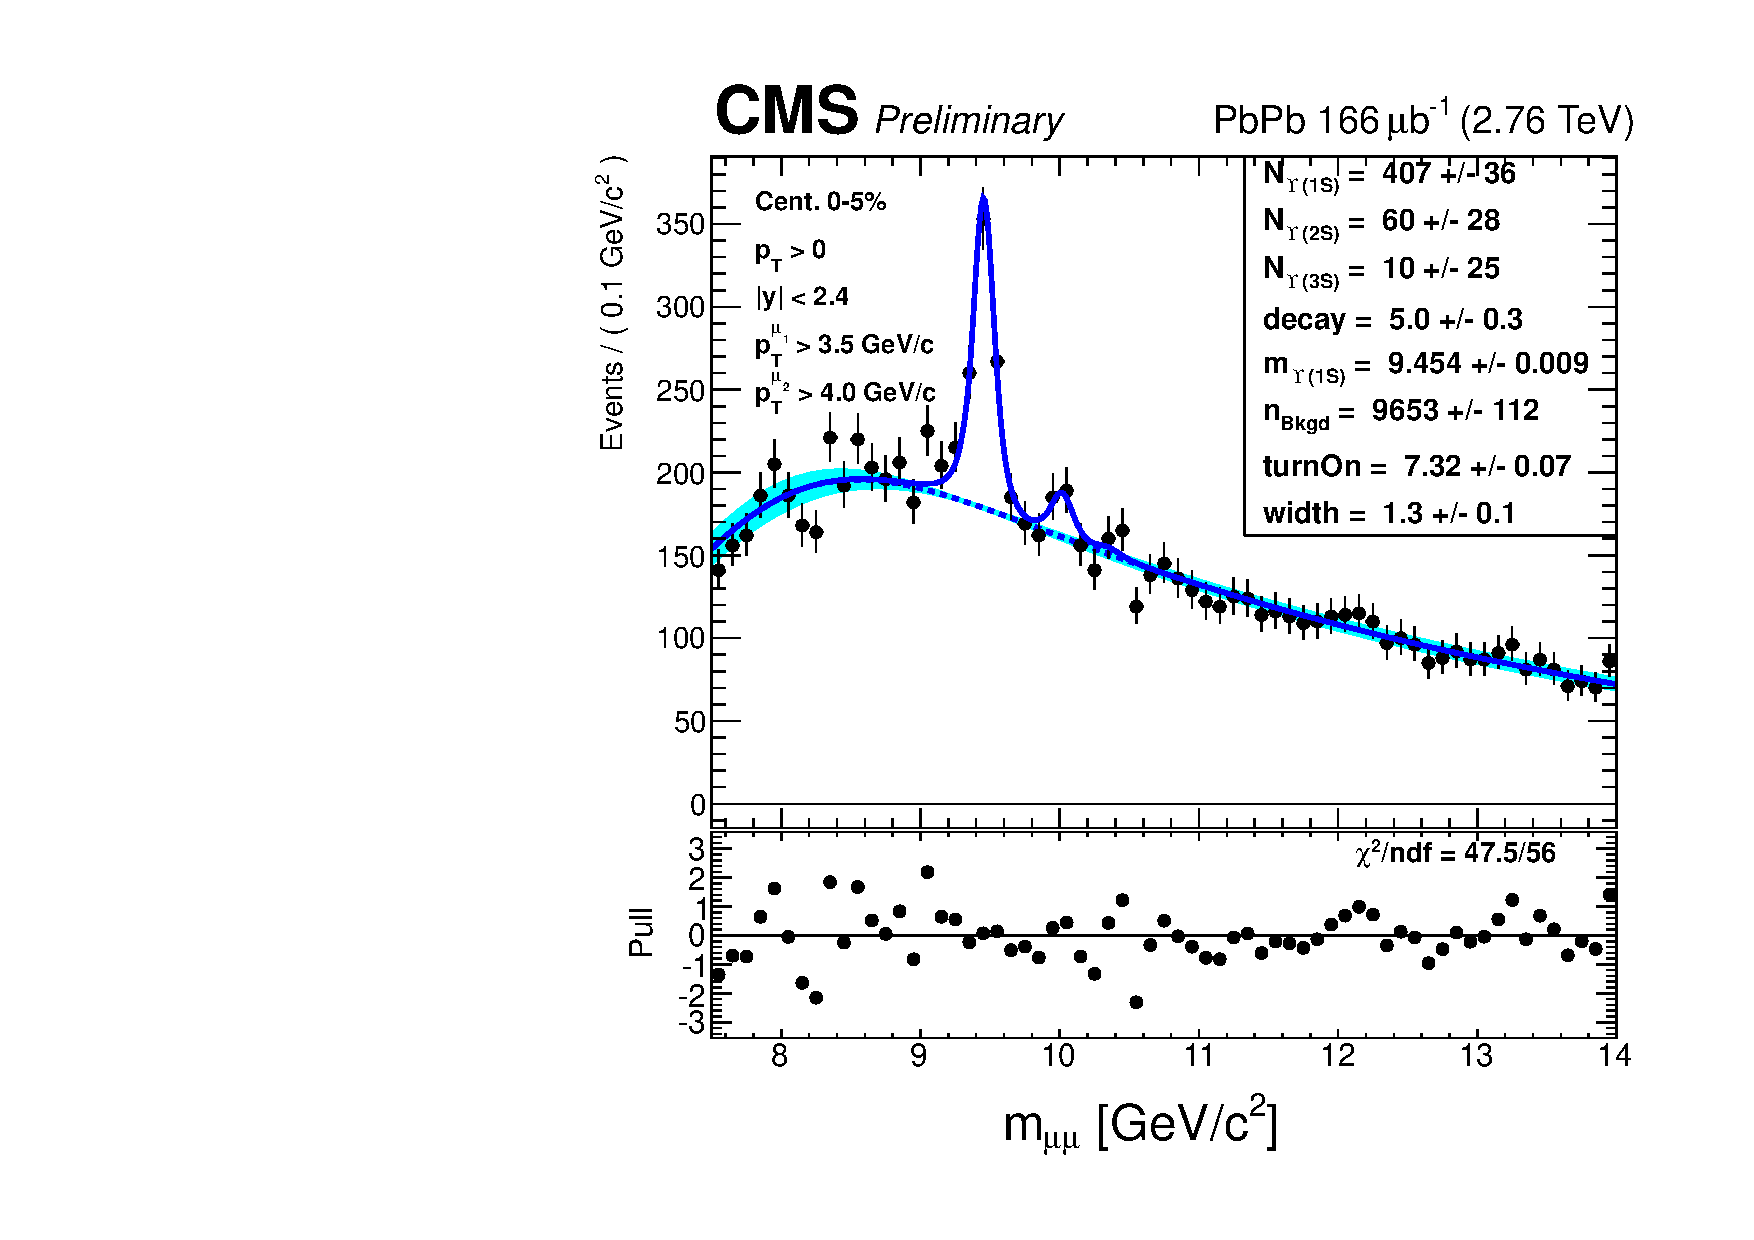
\includegraphics[width=0.49\textwidth]{Chapters/aYield/PbPb/pt_3p5_4/Centrality/Cent_0_5/PbPb_Cent_0_5_fsr1.pdf}
  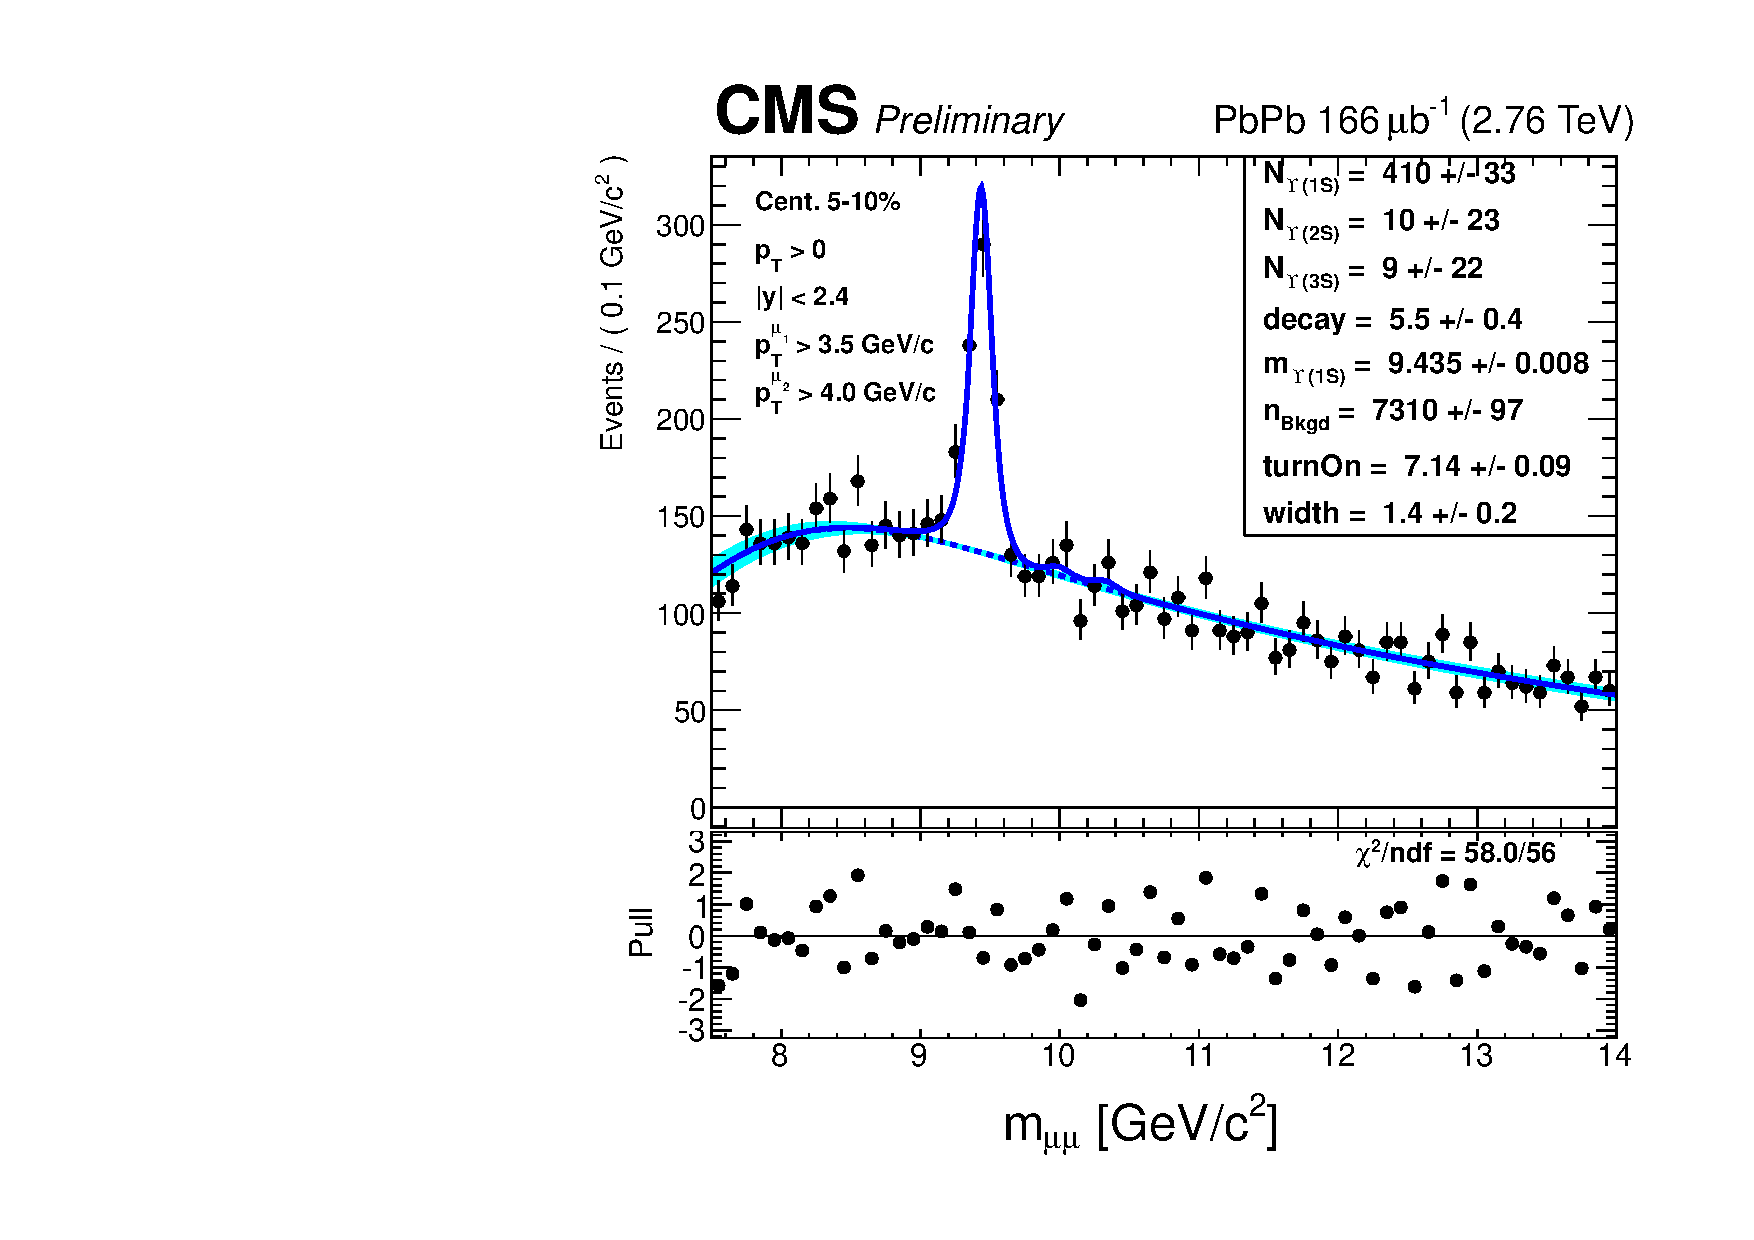
\includegraphics[width=0.49\textwidth]{Chapters/aYield/PbPb/pt_3p5_4/Centrality/Cent_5_10/PbPb_Cent_5_10_fsr1.pdf}
  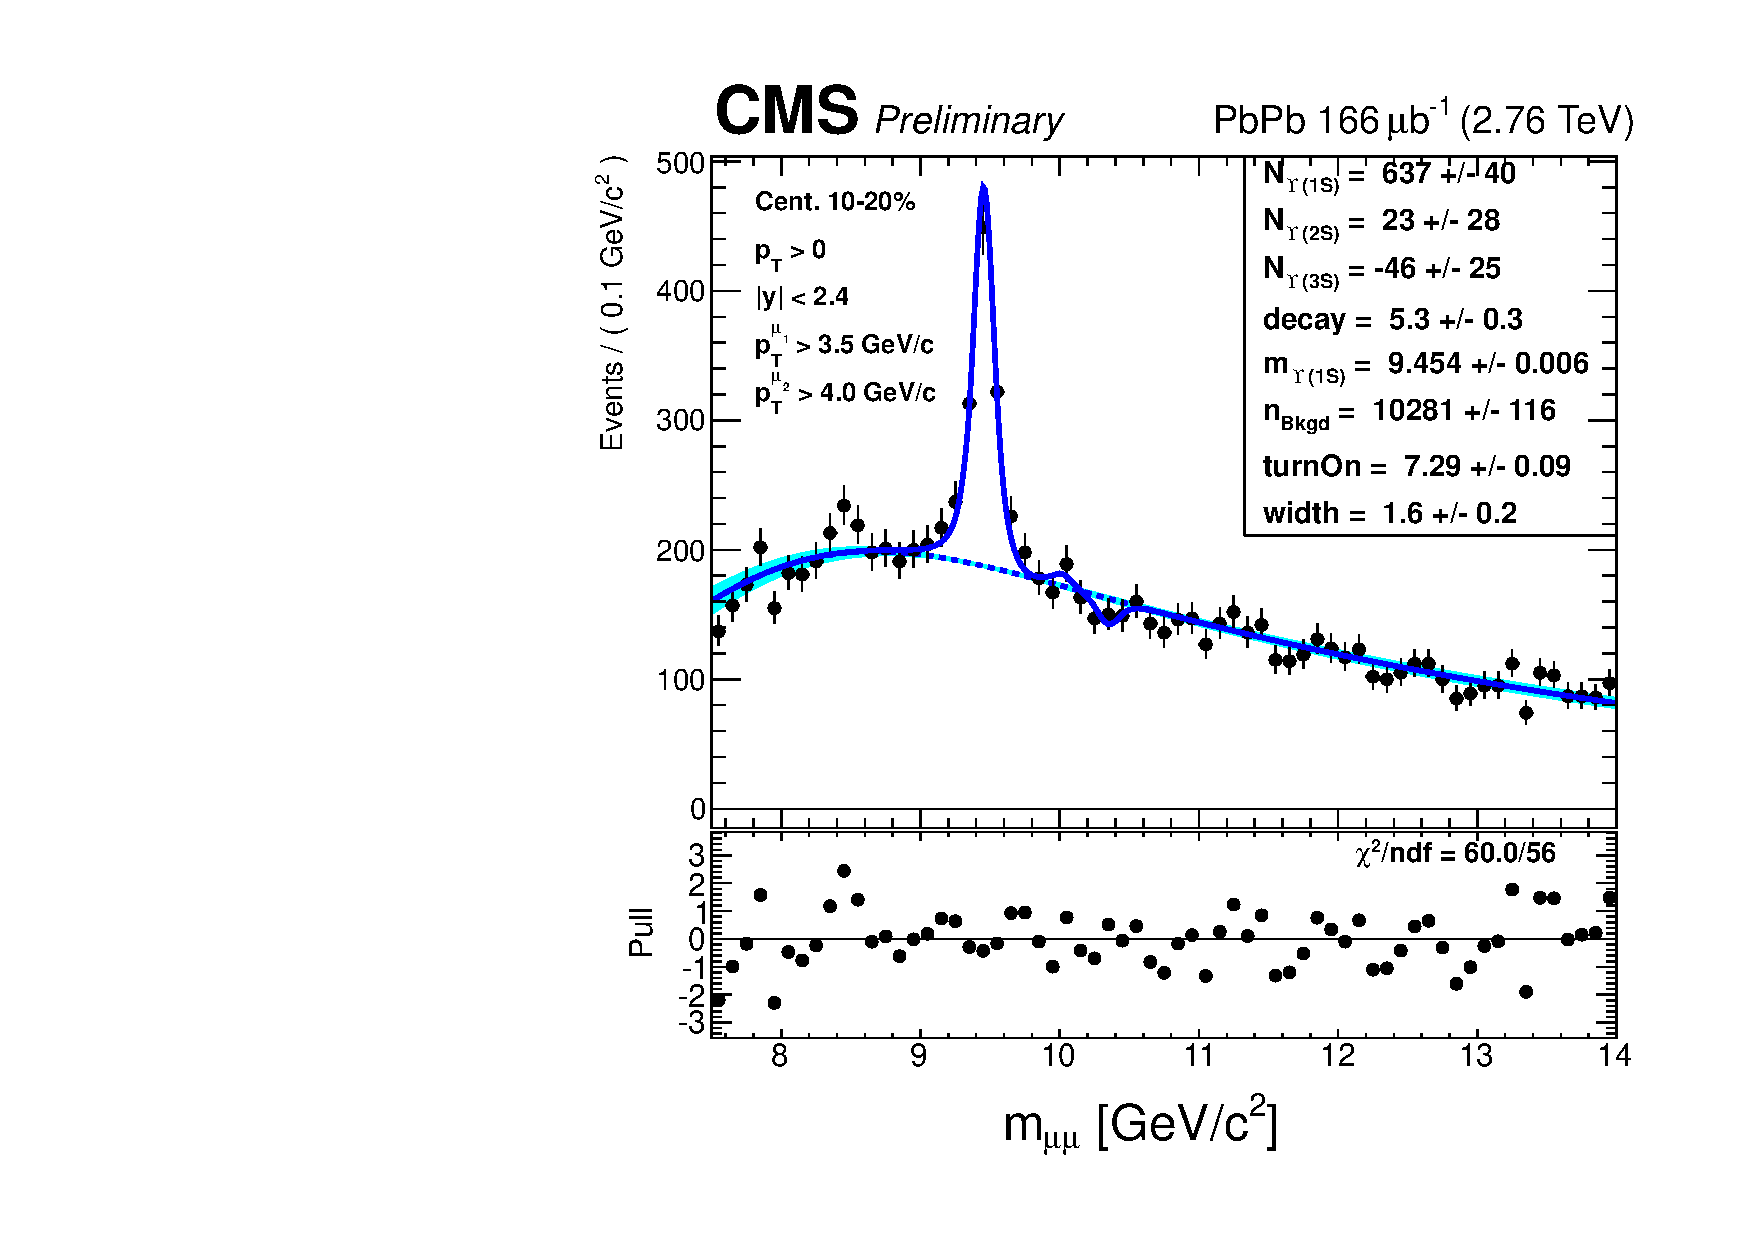
\includegraphics[width=0.49\textwidth]{Chapters/aYield/PbPb/pt_3p5_4/Centrality/Cent_10_20/PbPb_Cent_10_20_fsr1.pdf}
  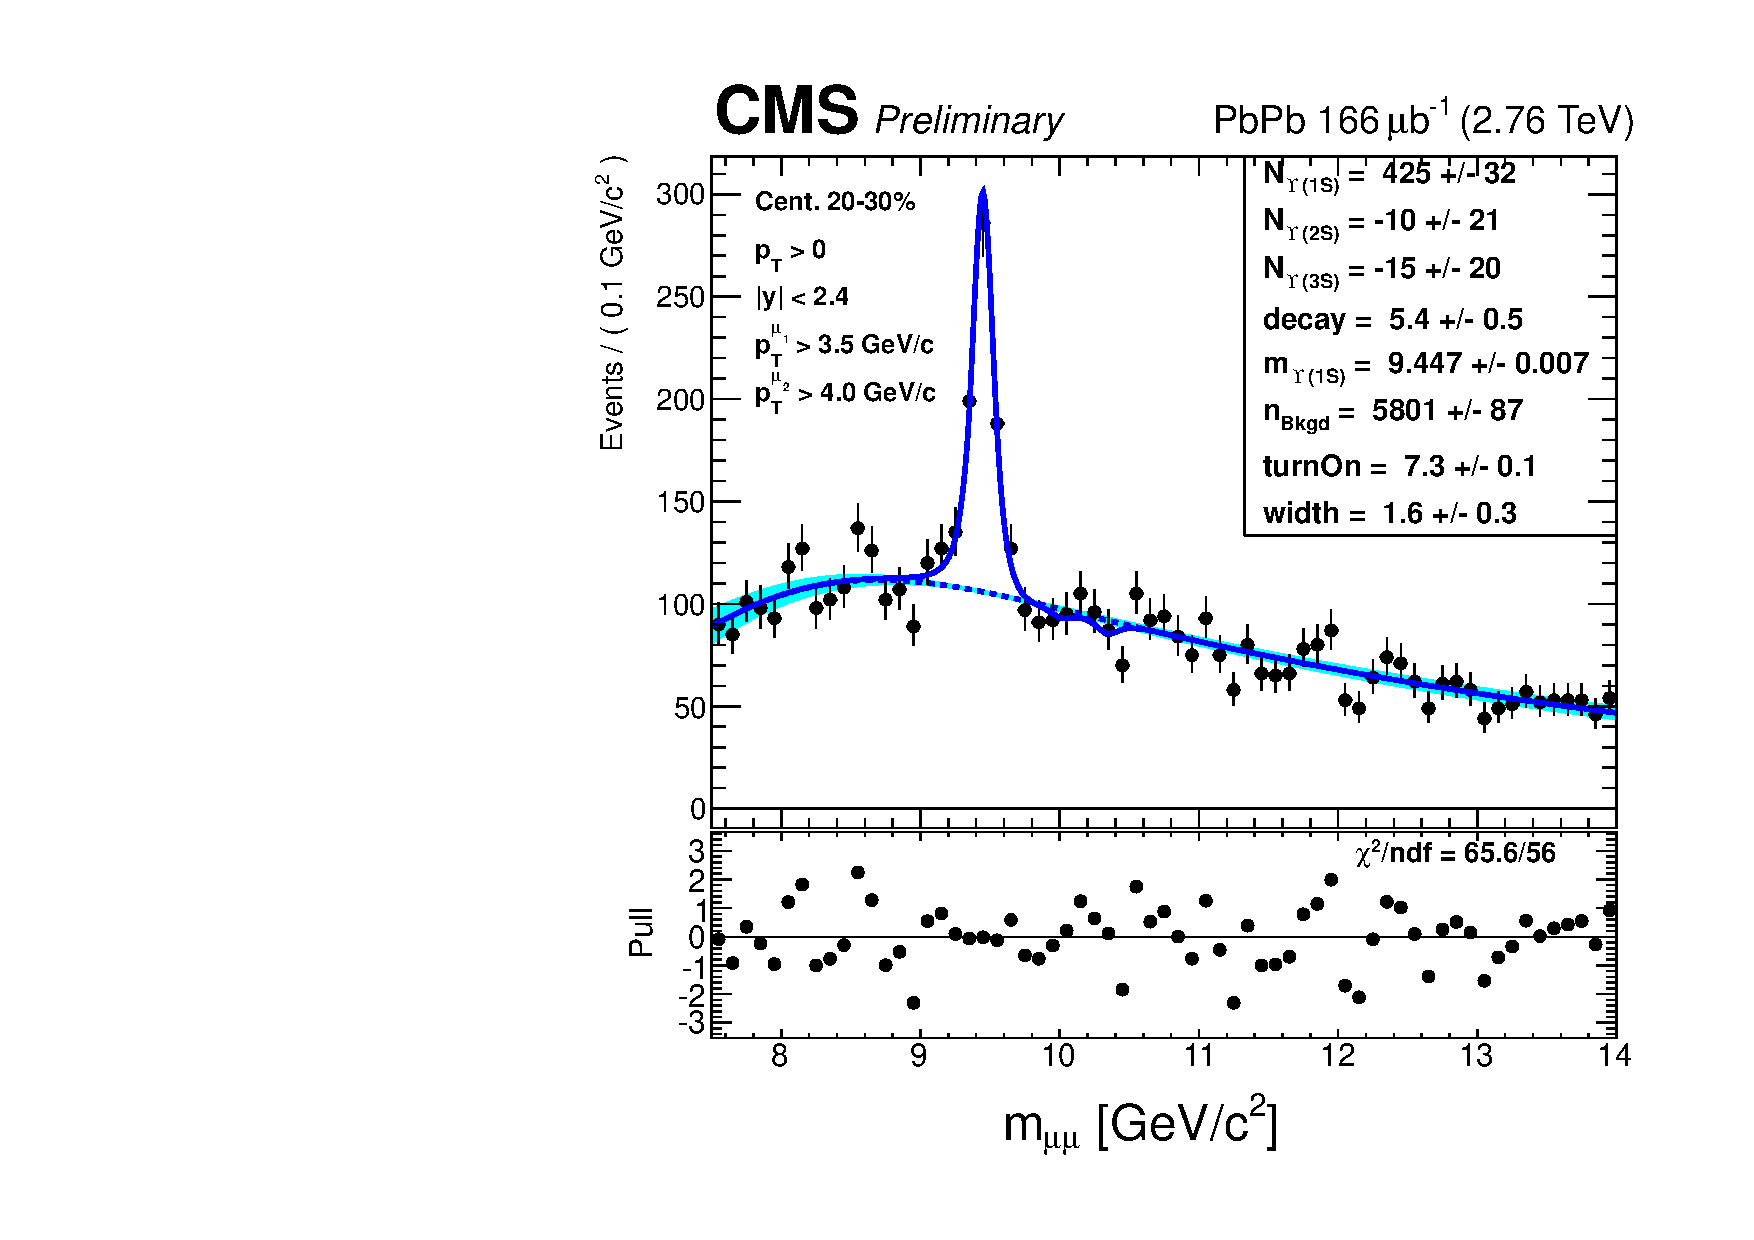
\includegraphics[width=0.49\textwidth]{Chapters/aYield/PbPb/pt_3p5_4/Centrality/Cent_20_30/PbPb_Cent_20_30_fsr1.pdf}
 \caption{Centrality-dependent fits to PbPb data (bins 0-5$\%$
   to 20-30$\%$)using loose muon
   pt cuts ($\PgUa$ analysis).}
 \label{fig:YieldsCent1S} 
\end{figure}
\begin{figure}
 \includegraphics[width=0.49\textwidth]{Chapters/aYield/PbPb/pt_3p5_4/Centrality/Cent_30_40/PbPb_Cent_30_40_fsr1.pdf}
 \includegraphics[width=0.49\textwidth]{Chapters/aYield/PbPb/pt_3p5_4/Centrality/Cent_40_50/PbPb_Cent_40_50_fsr1.pdf}
  \includegraphics[width=0.49\textwidth]{Chapters/aYield/PbPb/pt_3p5_4/Centrality/Cent_50_70/PbPb_Cent_50_70_fsr1.pdf}
  \includegraphics[width=0.49\textwidth]{Chapters/aYield/PbPb/pt_3p5_4/Centrality/Cent_70_100/PbPb_Cent_70_100_fsr1.pdf}
 \caption{Centrality-dependent fits to PbPb data (Continued:
   from 20-30 to 70-100$\%$ Centrality) using loose muon cuts ($\PgUa$ analysis).}
 \label{fig:YieldsCent1SContd} 
\end{figure}

\begin{figure}
  \includegraphics[width=0.49\textwidth]{Chapters/aYield/PbPb/pt_4_4/Centrality/Cent_0_10/PbPb_Cent_0_10_fsr1.pdf}
  \includegraphics[width=0.49\textwidth]{Chapters/aYield/PbPb/pt_4_4/Centrality/Cent_10_30/PbPb_Cent_10_30_fsr1.pdf}
  \includegraphics[width=0.49\textwidth]{Chapters/aYield/PbPb/pt_4_4/Centrality/Cent_30_50/PbPb_Cent_30_50_fsr1.pdf}
  \includegraphics[width=0.49\textwidth]{Chapters/aYield/PbPb/pt_4_4/Centrality/Cent_50_100/PbPb_Cent_50_100_fsr1.pdf}
 \caption{Centrality-dependent fits to PbPb data (bins 0-10$\%$,
   10-30, 30-50,
  50-100$\%$)using tight muon
   pt cuts ($\PgUb$ analysis).}
 \label{fig:YieldsCent2S} 
\end{figure}

\subsection{Systematic uncertainty on fitting}
\label{sec:figs_syst}
\begin{figure}
\begin{center}
  \includegraphics[width=0.45\textwidth]{Chapters/aYield/pp/pt_3p5_4/Rap/Rap_0_2p4/pp2p76tev_Rap_0_2p4_fsr1.pdf}
  \includegraphics[width=0.45\textwidth]{Chapters/aYield/pp/pt_3p5_4/Rap/Rap_0_2p4/pp2p76tev_Rap_0_2p4_fsr2.pdf}
  \includegraphics[width=0.45\textwidth]{Chapters/aYield/pp/pt_3p5_4/Rap/Rap_0_2p4/pp2p76tev_Rap_0_2p4_fsr3.pdf}
  \includegraphics[width=0.45\textwidth]{Chapters/aYield/pp/pt_3p5_4/Rap/Rap_0_2p4/pp2p76tev_Rap_0_2p4_fsr4.pdf}
  \includegraphics[width=0.45\textwidth]{Chapters/aYield/pp/pt_3p5_4/Rap/Rap_0_2p4/pp2p76tev_Rap_0_2p4_fsr5.pdf}
  \includegraphics[width=0.45\textwidth]{Chapters/aYield/pp/pt_3p5_4/Rap/Rap_0_2p4/pp2p76tev_Rap_0_2p4_fsr6.pdf}
 \caption{Fit Variations of the all-integrated pp data, cases where
   the signal shape was varied.}
 \label{fig:fitVar_ppMB-1}
\end{center}
\end{figure}
\begin{figure}
\begin{center}
  \includegraphics[width=0.45\textwidth]{Chapters/aYield/pp/pt_3p5_4/Rap/Rap_0_2p4/pp2p76tev_Rap_0_2p4_fsr1__bkg1.pdf}
  \includegraphics[width=0.45\textwidth]{Chapters/aYield/pp/pt_3p5_4/Rap/Rap_0_2p4/pp2p76tev_Rap_0_2p4_fsr1__bkg2.pdf}
 \caption{Fit Variations of the all-integrated pp data,
   continued. Cases where additional background components were
   tried.}
 \label{fig:fitVar_ppMB-2}
\end{center}
\end{figure}



\begin{figure}
\begin{center}
  \includegraphics[width=0.45\textwidth]{Chapters/aYield/PbPb/pt_3p5_4/Rap/Rap_0_2p4/PbPb_Rap_0_2p4_fsr1.pdf}
  \includegraphics[width=0.45\textwidth]{Chapters/aYield/PbPb/pt_3p5_4/Centrality/Cent_0_100/PbPb_Cent_0_100_fsr2.pdf}
  \includegraphics[width=0.45\textwidth]{Chapters/aYield/PbPb/pt_3p5_4/Centrality/Cent_0_100/PbPb_Cent_0_100_fsr3.pdf}
  \includegraphics[width=0.45\textwidth]{Chapters/aYield/PbPb/pt_3p5_4/Centrality/Cent_0_100/PbPb_Cent_0_100_fsr4.pdf}
  \includegraphics[width=0.45\textwidth]{Chapters/aYield/PbPb/pt_3p5_4/Centrality/Cent_0_100/PbPb_Cent_0_100_fsr5.pdf}
  \includegraphics[width=0.45\textwidth]{Chapters/aYield/PbPb/pt_3p5_4/Centrality/Cent_0_100/PbPb_Cent_0_100_fsr6.pdf}
 \caption{Fit Variations of the all-integrated PbPb data, cases where
   the signal shape was varied.}
 \label{fig:fitVar_AAMB-1}
\end{center}
\end{figure}


\begin{figure}
\begin{center}
  \includegraphics[width=0.45\textwidth]{Chapters/aYield/PbPb/pt_3p5_4/Centrality/Cent_0_100/PbPb_Cent_0_100_fsr1__bkg1.pdf}
  \includegraphics[width=0.45\textwidth]{Chapters/aYield/PbPb/pt_3p5_4/Centrality/Cent_0_100/PbPb_Cent_0_100_fsr1__bkg2.pdf}
 \caption{Fit Variations of the all-integrated PbPb data,
   continued. Casses where additional background components were
   tried.}
 \label{fig:fitVar_AAMB-2}
\end{center}
\end{figure}

\clearpage

\section{More figures from the MC lineshape study}
\label{sec:figs_mc}
Following Figures~\ref{fig:fsrFitPyquenRap}, Figures~\ref{fig:fsrFitPyquenRap2}
and~\ref{fig:fsrFitPyquenPt}, ~\ref{fig:fsrFitPyquenPt2} present \pt\ binned and rapidity binned
fits of the MC \PgUa\ simulation, used to estimate the lineshape
parameters to be used in the nominal signal extraction on data.
\begin{figure}
\begin{center}
\includegraphics[width=0.45\textwidth]{Chapters/aYield/MCpars_Pyquen_cent0M100_bkgModel0_sigModel4_muonEtaM240240_muonPt350M400_dimuPt000250_dimuY000240_trkRot0_constrain0_fsr0_sigma0_ref0_pulls.pdf}  
\includegraphics[width=0.45\textwidth]{Chapters/aYield/MCpars_Pyquen_cent0M100_bkgModel0_sigModel4_muonEtaM240240_muonPt350M400_dimuPt250500_dimuY000240_trkRot0_constrain0_fsr0_sigma0_ref0_pulls.pdf}
\includegraphics[width=0.45\textwidth]{Chapters/aYield/MCpars_Pyquen_cent0M100_bkgModel0_sigModel4_muonEtaM240240_muonPt350M400_dimuPt500800_dimuY000240_trkRot0_constrain0_fsr0_sigma0_ref0_pulls.pdf}
\includegraphics[width=0.45\textwidth]{Chapters/aYield/MCpars_Pyquen_cent0M100_bkgModel0_sigModel4_muonEtaM240240_muonPt350M400_dimuPt8001200_dimuY000240_trkRot0_constrain0_fsr0_sigma0_ref0_pulls.pdf} 
\includegraphics[width=0.45\textwidth]{Chapters/aYield/MCpars_Pyquen_cent0M100_bkgModel0_sigModel4_muonEtaM240240_muonPt350M400_dimuPt12002000_dimuY000240_trkRot0_constrain0_fsr0_sigma0_ref0_pulls.pdf}
\caption{$p_{T}$-binned fits of $\Upsilon$(1S) mass from a simulated
  sample embedded in events generated with
  HYDJET(Bass) for 1S bins.}
\label{fig:fsrFitPyquenPt}
\end{center}
\end{figure}

\begin{figure}
\begin{center} 
\includegraphics[width=0.45\textwidth]{Chapters/aYield/MCpars_Pyquen_cent0M100_bkgModel0_sigModel4_muonEtaM240240_muonPt350M400_dimuPt000500_dimuY000240_trkRot0_constrain0_fsr0_sigma0_ref0_pulls.pdf}
\includegraphics[width=0.45\textwidth]{Chapters/aYield/MCpars_Pyquen_cent0M100_bkgModel0_sigModel4_muonEtaM240240_muonPt350M400_dimuPt5001200_dimuY000240_trkRot0_constrain0_fsr0_sigma0_ref0_pulls.pdf}  
%\includegraphics[width=0.45\textwidth]{Chapters/aYield/MCpars_Pyquen_cent0M100_bkgModel0_sigModel4_muonEtaM240240_muonPt350M400_dimuPt12002000_dimuY000240_trkRot0_constrain0_fsr0_sigma0_ref0_pulls.pdf}
%\includegraphics[width=0.45\textwidth]{Chapters/aYield/MCpars_Pyquen_cent0M100_bkgModel0_sigModel4_muonEtaM240240_muonPt350M400_dimuPt20005000_dimuY000240_trkRot0_constrain0_fsr0_sigma0_ref0_pulls.pdf}
\caption{$p_{T}$-binned fits of $\Upsilon$(1S) mass from a simulated
  sample embedded in events generated with
  HYDJET(Bass) for 2S bins.}
\label{fig:fsrFitPyquenPt2}
\end{center}
\end{figure}

\begin{figure}
\begin{center}
\includegraphics[width=0.45\textwidth]{Chapters/aYield/MCpars_Pyquen_cent0M100_bkgModel0_sigModel4_muonEtaM240240_muonPt350M400_dimuPt0005000_dimuY000040_trkRot0_constrain0_fsr0_sigma0_ref0_pulls.pdf} 
\includegraphics[width=0.45\textwidth]{Chapters/aYield/MCpars_Pyquen_cent0M100_bkgModel0_sigModel4_muonEtaM240240_muonPt350M400_dimuPt0005000_dimuY040080_trkRot0_constrain0_fsr0_sigma0_ref0_pulls.pdf}
\includegraphics[width=0.45\textwidth]{Chapters/aYield/MCpars_Pyquen_cent0M100_bkgModel0_sigModel4_muonEtaM240240_muonPt350M400_dimuPt0005000_dimuY080120_trkRot0_constrain0_fsr0_sigma0_ref0_pulls.pdf}
\includegraphics[width=0.45\textwidth]{Chapters/aYield/MCpars_Pyquen_cent0M100_bkgModel0_sigModel4_muonEtaM240240_muonPt350M400_dimuPt0005000_dimuY120160_trkRot0_constrain0_fsr0_sigma0_ref0_pulls.pdf} 
\caption{Rapidity-binned fits of $\Upsilon$(1S) mass from a simulated
  sample embedded in events generated with
  HYDJET(Bass) (Entries 1 to 6 for 1S bins, entries 7 and 8 for 2S bins).}
\label{fig:fsrFitPyquenRap}
\end{center}
\end{figure}

\begin{figure}
\begin{center}
\includegraphics[width=0.45\textwidth]{Chapters/aYield/MCpars_Pyquen_cent0M100_bkgModel0_sigModel4_muonEtaM240240_muonPt350M400_dimuPt0005000_dimuY160200_trkRot0_constrain0_fsr0_sigma0_ref0_pulls.pdf}
\includegraphics[width=0.45\textwidth]{Chapters/aYield/MCpars_Pyquen_cent0M100_bkgModel0_sigModel4_muonEtaM240240_muonPt350M400_dimuPt0005000_dimuY200240_trkRot0_constrain0_fsr0_sigma0_ref0_pulls.pdf}
\includegraphics[width=0.45\textwidth]{Chapters/aYield/MCpars_Pyquen_cent0M100_bkgModel0_sigModel4_muonEtaM240240_muonPt350M400_dimuPt0005000_dimuY000120_trkRot0_constrain0_fsr0_sigma0_ref0_pulls.pdf}
\includegraphics[width=0.45\textwidth]{Chapters/aYield/MCpars_Pyquen_cent0M100_bkgModel0_sigModel4_muonEtaM240240_muonPt350M400_dimuPt0005000_dimuY120240_trkRot0_constrain0_fsr0_sigma0_ref0_pulls.pdf}
\caption{Same as Figure~\ref{fig:fsrFitPyquenRap}, continued
  Rapidity-binned fits for high rapidity 1S bins, and for wide 2S bins.}
\label{fig:fsrFitPyquenRap2}
\end{center}
\end{figure}

Figure~\ref{fig:likelihoodScanExampleHiRap} shows the likelihood scan
of fit variables in the range $2.4 < \vert\y\vert < 2.4$.

\begin{figure}
\begin{center}
\includegraphics[width=1\textwidth]{Chapters/aYield/likelihoodScanExampleRap2-2p4.pdf}  
\caption{A not so good likelihood scan of the 2$<|$y$|< $ 2.4 $\Upsilon$(1S)
  subsample.}
\label{fig:likelihoodScanExampleHiRap}
\end{center}
\end{figure}
\section{Tabulated results of the lineshape study}

\begin{table}

    \begin{tabular}{c|c|c|c|c|c}
      \hline
      $\Sigma$ parameters &  \multicolumn{2}{c}{power-law} \vline& \multicolumn{3}{c}{the rest}  \\                                               
      \hline
      Bin & n$_{CB}$ & $\alpha_{CB}$ & $\sigma_{1}$(MeV) & $x$ (scale) & $f$ (norm) \\  
      \hline                                                                                                   
      pt$<$2.5    &11.86  & 1.322  & 0.0651  & 1.766  & 0.552 \\ 
      2.5$<$pt$<$5&17.39  & 1.312  & 0.0654  & 1.798  & 0.562\\ 
      5$<$pt$<$8  &28.63  & 1.197  & 0.0691  & 1.747  & 0.655 \\ 
      8$<$pt$<$12 &21.34  & 1.418  & 0.0675  & 1.664  & 0.541 \\ 
      12$<$pt$<$20&40.28  & 1.165  & 0.0679  & 1.824  & 0.661 \\ 
     % 20$<$pt$<$50&2.7$\pm$0.4&1.55$\pm$0.04&71$\pm$0.8&1.93$\pm$0.03&0.70$\pm$0.01&9456.7$\pm$0.4\\ 
      \hline
      0$<|$y$|<$0.4  &7.433  & 1.339  & 0.0445 & 1.472  & 0.448 \\ 
      0.4$<|$y$|<$0.8&1.449  & 1.895  & 0.0694 & 2.160  & 0.964 \\ 
      0.8$<|$y$|<$1.2&3.048  & 1.631  & 0.0769 & 1.410  & 0.559 \\ 
      1.2$<|$y$|<$1.6&8.799  & 1.725  & 0.0871 & 1.496  & 0.512 \\ 
      1.6$<|$y$|<$2.0&2.512  & 1.930  & 0.1272 & 2.033  & 0.991 \\
      2.0$<|$y$|<$2.4&36.89  & 1.408  & 0.1448 & 1.223  & 0.698\\ 
      \hline
      pt$<$5       &28.30  & 1.280  & 0.0662  & 1.83 & 0.619\\
      5$<$pt$<$12  &25.03  & 1.257  & 0.0664  & 1.86 & 0.637 \\ 
      12$<$pt$<$20 &3.092  & 1.605  & 0.0706  & 1.58 & 0.575\\ 
      \hline
      0$<|$y$|<$1.2  &13.44  & 1.323 & 0.0556 & 1.662  & 0.577\\ 
      1.2$<|$y$|<$2.4&11.87  & 1.667 & 0.1020 & 1.515  & 0.647\\ 
      \hline
      Min.Bias(loose pt) & 2.452 & 1.650  & 0.0670  & 1.85 & 0.603 \\ 
      Min.Bias(tight pt) & 4.651 & 1.559  & 0.0655  & 1.83 & 0.582 \\ 
      \hline
\end{tabular}

\caption{Fit results of signal shape parameters.} 
\label{tab:FSRparameters}
 \end{table}
